% Začetek preambule
\documentclass[a4paper, 12pt]{amsart}
\usepackage[slovene]{babel}
\usepackage[utf8]{inputenc}
\usepackage[T1]{fontenc}
\usepackage{lmodern}
\usepackage{amsfonts,amsmath,amssymb}
\usepackage{graphicx}
\usepackage{url}
\usepackage{tikz}
\usepackage{subfigure}
\usepackage{hyperref}

% ne spreminjaj podatkov, ki vplivajo na obliko strani
\textwidth 15cm
\textheight 24cm
\oddsidemargin.5cm
\evensidemargin.5cm
\topmargin-5mm
\addtolength{\footskip}{10pt}
\pagestyle{plain}
\overfullrule=15pt % oznaci predlogo vrstico


% ukazi za matematicna okolja
\theoremstyle{definition} % tekst napisan pokoncno
\newtheorem{definicija}{Definicija}[section]
\newtheorem{primer}[definicija]{Primer}
\newtheorem{opomba}[definicija]{Opomba}

\newtheorem{zgled}[definicija]{Zgled}

\theoremstyle{plain} % tekst napisan posevno
\newtheorem{lema}[definicija]{Lema}
\newtheorem{izrek}[definicija]{Izrek}
\newtheorem{trditev}[definicija]{Trditev}
\newtheorem{posledica}[definicija]{Posledica}


% simboli za stevilske mnozice 
\newcommand{\R}{\mathbb R}
\newcommand{\N}{\mathbb N}
\newcommand{\Z}{\mathbb Z}
\newcommand{\C}{\mathbb C}
\newcommand{\Q}{\mathbb Q}
\newcommand{\F}{\mathbb F}
\newcommand{\M}{\mathbb M}

% ukazi za prvo stran
\newcommand{\program}{Matematika } % ime studijskega programa: Matematika
\newcommand{\imeavtorja}{Klemen Pavlič} % ime avtorja
\newcommand{\imementorja}{izr.~prof.~dr. David Dolžan} % akademski naziv in ime mentorja
\newcommand{\naslovdela}{Grafi deliteljev niča in totalni grafi kolobarjev}
\newcommand{\letnica}{2014} %letnica diplome

% moje definicije ...
\DeclareMathOperator{\aut}{Aut}
\DeclareMathOperator{\ann}{ann}
\DeclareMathOperator{\diam}{diam}
\DeclareMathOperator{\nil}{Nil}
\DeclareMathOperator{\dist}{dist}
\DeclareMathOperator{\GF}{GF}
\DeclareMathOperator{\deter}{det}


% začetek dokumenta
\begin{document}
\thispagestyle{empty}
\noindent{\large
UNIVERZA V LJUBLJANI\\[1mm]
FAKULTETA ZA MATEMATIKO IN FIZIKO\\[5mm]
\program -- 2.~stopnja}
\vfill

\begin{center}{\large
\imeavtorja\\[2mm]
{\bf \naslovdela}\\[10mm]
Magistrsko delo\\[1cm]
Mentor: \imementorja}
\end{center}
\vfill

\noindent{\large
Ljubljana, \letnica}
\pagebreak

\thispagestyle{empty}
\tableofcontents
\pagebreak

\thispagestyle{empty}
\begin{center}
{\bf \naslovdela}\\[3mm]
{\sc Povzetek}
\end{center}
% tekst povzetka v slovenscini
Tekst povzetka v slovenščini.
\vfill
\begin{center}
{\bf Title}\\[3mm] % prevod slovenskega naslova dela 
{\sc Abstract}
\end{center}
% tekst povzetka v anglescini
Tekst povzetka v angleščini.

\vfill\noindent
{\bf Math. Subj. Class. (2010):} 05C25, 05C12, 05C15, 05C45  \\[1mm]  
{\bf Klju"cne besede:} graf deliteljev niča, totalni graf,  barvanje povezav,  Eulerjev graf, ravninski graf
 \\[1mm]  
{\bf Keywords:} zero-divisor graph, total graph, edge coloring, Eulerian graph, planar graph
\pagebreak

% UVOD
\section{Uvod}

% JACOBSONOV RADIKAL
\section{Jacobsonov radikal}

\begin{definicija} 
Naj bo $R$ poljuben kolobar. Potem je \emph{Jacobsonov radikal} $J(R)$ enak preseku vseh maksimalnih levih idealov kolobarja $R$.
\end{definicija}
Najprej opazimo, da v komutativnih kolobarjih zgornja definicija sovpada z definicijo iz \cite{diploma}, kjer je Jacobsonov radikal komutativnega kolobarja definiran kot presek vseh maksimalnih idealov.

Poglejmo si zdaj, kaj velja za elemente iz Jacobsonovega radikala.
\begin{lema}
\label{J(R)-prvic}
Naj bo $R$ enotski kolobar, ki ni nujno komutativen. Potem so za $y\in R$ ekvivalentne naslednje trditve
 \begin{enumerate}
 \item $y\in J(R)$,
\item $1-xy$ ima levi inverz za vsak $x\in R$,
\item $ yM = 0$ za vsak enostaven levi $R$-modul $M$.
\end{enumerate}
\end{lema}

\proof
Dokažimo implikacijo $(1) \Rightarrow (2)$. Naj bo $y\in J(R)$. Denimo, da implikacija ne velja. Potem obstaja $x\in R$, da $1-xy$ nima levega inverza. Potem je $R(1-xy) \subsetneq R$ in $R(1-xy)$ je vsebovan v nekem maksimalnem levem idealu $m$. Ker pa je $1-xy \in R(1-xy) \subseteq m$, je $1-xy\in m$. Poleg tega je $y\in J(R) \subseteq m$ in zato je tudi $xy \in m$. Sledi $1\in m$. Protislovje.

Dokažimo implikacijo $(2) \Rightarrow (3)$. Naj bo torej $M$ enostaven levi $R$-modul. Naj bo $m\in M$ tak, da je $ym \neq 0$. Ker je $M$ enostaven, mora biti torej $R\cdot ym = M$. Potem obstaja $x\in R$, da je $m = x\cdot ym$. To zvezo lahko prepišemo v $(1-xy)m=0$. Po predpostavki ima $1-xy$ levi inverz in če zgornjo zvezo pomnožimo z njim, dobimo $m=0$. Protislovje s predpostavko, da je $ym\neq 0$.

Dokažimo še implikacijo $(3) \Rightarrow (1)$. Naj bo $m$ poljuben maksimalen levi ideal. Potem je $R/m$ enostaven levi $R$ -modul. Po predpostavki je potem $y  \cdot R/m = 0$, kar implicira, da je $y\in m$. Ker je bil zgoraj $m$ poljuben, je potem $y\in J(R)$.
\endproof

Spomnimo se, da je za poljuben levi $R$-modul $M$ anihilator $M$ definiran kot $\ann(M) = \{r\in R: rM = 0\}$. To je očitno ideal kolobarja $R$. Če sta $a,b\in \ann(M)$ in $r\in R$, potem je jasno $a+b, ra\in \ann(M)$, prav tako pa je $ar\in \ann(M)$, saj je $ar\cdot M = a \cdot rM \subseteq a M =0$.

Naj bo zdaj $I$ levi ideal kolobarja $R$. Za $R$-modul $M$ lahko vzamemo kar $R/I$. Potem je $\ann(M) = \{r\in R: r\cdot R/I = 0\} = \{ r\in R: rR \subseteq I\}$.

Zdaj lahko zapišemo takojšnjo posledico zgornje leme in zgoraj zapisanega. 
\begin{posledica}
\label{J(R)-presekAnihilatorjev}
Naj bo $R$ enotski kolobar. Potem je Jacobsonov radikal $J(R) = \cap \ann(M)$, kjer presek teče po vseh enostavnih levih $R$-modulih. Sledi še, da je $J(R)$ ideal v $R$.
\end{posledica}

S pomočjo te posledice lahko dokažemo še naslednjo ekvivalentno definicijo Jacobsonovega radikala.

\begin{lema}
\label{J(R)-drugic}
Naj bo $R$ enotski kolobar. Potem sta za $y\in R$ ekvivalentni trditvi
\begin{enumerate}
\item $y\in J(R)$ in 
\item $1 - xyz \in U(R)$ za vsaka $x,z\in R$.
\end{enumerate}
\end{lema}

\proof
Dokažimo najprej implikacijo iz $(2) \Rightarrow (1)$. Ker $(2)$ velja za vsak $z$, velja tudi za $z=1$. Potem je $1- xy\in U(R)$ za vsak $x\in R$ in po \ref{J(R)-prvic} je $y\in J(R)$. 

Dokažimo še $(1) \Rightarrow (2)$. Naj bo torej $y\in J(R)$ in $x,z\in R$. Ker je po \ref{J(R)-presekAnihilatorjev} $J(R)$ ideal, je $yz\in J(R)$. Zato po \ref{J(R)-prvic} obstaja $u\in R$, da je $u (1-xyz) = 1$. Od tod sledi še, da ima $u$ desni inverz. Ker pa je po \ref{J(R)-presekAnihilatorjev} tudi $xyz\in J(R)$, ima po \ref{J(R)-prvic}  $u = 1+ u(xyz)$ še levi inverz. Sledi torej, da je $u\in U(R)$ in posledično $1-xyz\in U(R)$.
\endproof

\begin{posledica}
Naj bo $R$ enotski kolobar. Potem je Jacobsonov radikal $J(R)$ največji levi ideal $I \subseteq R$, ki zadošča $1+I\subseteq U(R)$.
\end{posledica}

\proof
Sledi iz \ref{J(R)-presekAnihilatorjev} in \ref{J(R)-drugic}.
\endproof

\begin{posledica}
Naj bo $R$ enotski kolobar in $I$ ideal v $R$, ki zadošča $I\subseteq J(R)$. Potem je $J(R/I) = J(R)/I$.
\end{posledica}

\proof
Sledi s pomočjo ekvivalence med (1) in (2) v \ref{J(R)-prvic}.
\endproof

Na tem mestu lahko omenimo Jacobsonovo polenostavnost. Pravimo, da je kolobar $R$ \emph{Jacobsonovo polenostaven} (oziroma \emph{J-polenostaven}), če je $J(R) = 0$. Primerov takih kolobarjev ni težko najti, saj je za poljuben kolobar $R$ kvocientni kolobar $R/J(R)$ $J$-polenostaven kolobar. Na ta način lahko vsakemu kolobarju priredimo $J$-polenostaven kolobar. Izkaže se, da imata kolobar in pripadajoči $J$-polenostavni kolobar nekatere lastnosti skupne, zato se včasih bolj splača obravnavati pripadajoči $J$-polenostavni kolobar.

\begin{lema}
\label{RinR/J(R)}
Naj bo $R$ enotski kolobar. Potem imata $R$ in $R/J(R)$ iste enostavne leve module. Prav tako velja, da je $x\in R$ levo obrnljiv (obrnljiv) v $R$ natanko tedaj, ko je $\overline{x} \in \overline{R} = R/J(R)$ levo obrnljiv (obrnljiv) v $\overline{R} = R/J(R)$.
\end{lema}

\proof
Prvi del leme sledi iz ekvivalence med $(1)$ in $(3)$ v \ref{J(R)-prvic}. Če ima $x$ levi inverz $y$, je jasno, da je $\overline{y}$ levi inverz $\overline{x}$. Pokazati moramo torej le še, da iz obstoja levega inverza elementa $\overline{x}$ sledi obstoj levega inverza  elementa $x$. Naj bo torej $y\in R$ tak, da je $\overline{y} \overline{x} = \overline{1}$. Potem je $1- yx \in J(R)$. To pa je ekvivalentno temu, da je $yx \in 1 + J(R) \subseteq U(R)$. Potem obstaja  $u\in R$, da je $u\cdot yx =1$ in je $uy $ levi inverz elementa $x$. Analogno dokažemo za desno obrnljivost.
\endproof

\begin{lema}
Naj bo $\{I_j\}_{j=1}^m$ neki končni nabor levih idealov kolobarja $R$. Če je vsak izmed njih nilpotenten, potem je tudi $I_1 + \dots + I_m$ nilpotenten.
\end{lema}

\proof
Zadošča obravnavati primer $m=2$, sicer pa uporabimo indukcijo. Naj bosta torej $I_1,I_2$ dva nilpotentna leva ideala. Naj bo $n\in \N$ najmanjši tak, da je $I_1^n = 0$ in $I_2^n = 0$. Označimo z $L=I_1 + I_2$. Trdimo, da je $L^{2n} = 0$. Pokazati moramo, da je produkt $2n$ elementov $(x_1 + y_1) \cdots (x_{2n} + y_{2n}), x_i \in I_1, y_i \in I_2$  enak 0. Ta produkt razpišemo. Vsak sumand bo produkt $2n$ členov, pri čemer jih bo vsaj $n$ iz $I_1$ ali vsaj $n$ iz $I_2$. Ker sta $I_1$ in $I_2$ leva ideala in ker je $I_1^n = 0 = I_2^n$, so vsi sumandi enaki 0 in zato je zgornji produkt res enak 0. Sledi $L^{2n} = 0$.
\endproof
 
Pravimo, da je ideal $I$ \emph{nil ideal}, če so vsi njegovi elementi nilpotentni. To pomeni, da za vsak $x\in I$ obstaja $n\in \N$, da je $x^n =0$. Jasno je, da je vsak nilpotentni ideal tudi nil ideal, obratna implikacija pa ne velja.
Analogno definiramo še pojem enostranskega nil ideala.

\begin{lema}
\label{nilPodJ(R)}
Naj bo $R$ enotski kolobar. Če je $I\subseteq R$ levi (desni) nil ideal, potem je $I\subseteq J(R)$.
\end{lema}

\proof
Naj bo $y\in I$. Ker je $I$ levi ideal, je za vsak $x\in R$ tudi $xy \in I$ in posledično je $xy$ nilpotenten. Obstaja torej $n\in \N$, da je $(xy)^n = 0$. Oglejmo si sedaj element $1-xy$. Ta ima inverz $\sum_{j=0}^{\infty} (xy)^j = \sum_{j=0}^{n-1} (xy)^j$. Po \ref{J(R)-prvic} je torej $y \in J(R)$. Dokaz gre podobno tudi v primeru, ko je $I$ desni nil ideal, le da si pomagamo z lemo \ref{J(R)-drugic}.
\endproof

Ker je vsak nilpotentni ideal očitno tudi nil ideal, nam zgornja lema pove, da $J(R)$ vsebuje vse nilpotentne leve ideale. V primeru artinskih kolobarjev pa lahko povemo še več. Pokazali bomo, da mora biti v tem primeru $J(R)$ kar nilpotenten.

\begin{izrek}
\label{J(R)nilpotenten-levoArtinski}
Naj bo $R$ levo artinski enotski kolobar. Potem je $J(R)$ največji nilpotentni levi ideal.
\end{izrek}

\proof
Po komentarju pred izrekom zadošča dokazati, da je $J(R)$ nilpotenten. Ker je $R$ levo artinski, obstaja naravno število $k$, da je $J(R)^k = J(R) ^{k+1} = I$. Trdimo, da je $I=0$. Denimo nasprotno, da $I\neq 0$. Poglejmo si množico $\mathcal{S}$ levih idealov $K$ v $R$, ki zadoščajo pogoju $I\cdot K \neq 0$. Množica $\mathcal{S}$ je neprazna, saj vsebuje $I$. Ker je $R$ levo artinski, ima $\mathcal{S}$ minimalni element $K_0$. Naj bo zdaj $a\in K_0$ tak element, da je $I\cdot a \neq 0$. Potem je $I\cdot (Ia) = I^2 a = Ia \neq 0$. Ker pa je $K_0$ minimalen, mora biti $Ia = K_0$. To pa pomeni, da je $a = ya$ za neki $y\in I \subseteq J(R)$. To zvezo lahko prepišemo v $(1-y)a = 0$. Ker je $y\in J(R)$, ima po \ref{J(R)-prvic} element $1-y$ levi inverz. To pomeni, da je $a=0$. Protislovje. Sledi, da je $J(R)^k = 0$.
\endproof

Če združimo lemo \ref{nilPodJ(R)} in izrek \ref{J(R)nilpotenten-levoArtinski}, dobimo naslednjo posledico.

\begin{posledica}
V levo artinskem enotskem kolobarju je vsak levi nil ideal nilpotenten.
\end{posledica}

Do sedaj smo ves čas govorili le o kolobarjih z enoto. Pojavi se vprašanje, kako smiselno definirati Jacobsonov radikal v kolobarijh brez enote. 

V ta namen bomo najprej uvedli pojem kvazi regularnega elementa. Pred tem pa moramo definirati še operacijo $\circ$. Naj bo torej $R$ poljuben kolobar (lahko je nekomutativen in brez enote). Za poljubna $x,y\in R$ definiramo $x\circ y = x+y-xy$. Z lahkoto preverimo, da je ta operacija asociativna, kar pomeni, da je za poljubne $x,y,z\in R$ izpolnjena enakost $x\circ(y\circ z) = (x\circ y) \circ z$. Očitno velja še $x \circ 0 = 0 \circ x = x$ in zato je $(R,\circ )$ asociativen monoid z enoto. Pri tem je $x\circ y = y\circ x$ natanko tedaj, ko je $xy = yx$.

\begin{definicija}
Naj bo $R$ kolobar. 
\begin{enumerate}
\item Element $x\in R $ je \emph{levo kvazi regularen}, če obstaja $y\in R$, da je $y\circ x=0$. Element $x\in R$ je \emph{desno kvazi regularen}, če obstaja $z\in R$, da je $x\circ z = 0$. Element $x\in R$ je \emph{kvazi regularen}, če je levo kvazi regularen in desno kvazi regularen. Pri tem elementu $y$ rečemo \emph{levi kvazi inverz}, elementu $z$ pa \emph{desni kvazi inverz}.
\item Levi ideal $I$ kolobarja $R$ je \emph{kvazi regularen}, če je vsak element $x\in I$ levo kvazi regularen.
\item Desni ideal $I$ kolobarja $R$ je \emph{kvazi regularen}, če je vsak element $x\in I$ desno kvazi regularen.
\end{enumerate}
\end{definicija}

Pokažimo sedaj naslednjo lemo, ki govori o kvazi regularnosti v kolobarju z enoto.

\begin{lema}
\label{kvaziRegularen-enotskiR}
Naj bo $R$ enotski kolobar. 
\begin{enumerate}
\item Element $x\in R$ je levo (desno) kvazi regularen natanko tedaj, ko ima $1-x$ levi (desni) inverz v $R$.
\item Element $x\in R$ je kvazi regularen natanko tedaj, ko je $1-x \in U(R)$.
\item Če je $I$ levi ali desni ideal, ki je kvazi regularen, potem je vsak element $x\in I$ kvazi regularen.
\end{enumerate}
\end{lema}

\proof
Dokazali bomo vsako točko leme posebej. Začnimo kar s prvo.
\begin{enumerate}
\item Naj bo $x$ levo kvazi regularen. Potem obstaja $y\in R$, da je $y\circ x = y+x - yx = 0$. To je ekvivalentno temu, da velja $1 = 1 -y-x + yx = (1-y)(1-x)$. To pa ravno  pomeni, da ima element $1-x$ levi inverz. Pokažimo še obrat. Naj bo torej $z(1-x) = 1$ za neki $z\in R$. Zapišimo $z$ kot $z = 1 -y$ za neki $y\in R$ (vzamemo lahko $y = 1-z$). Potem je $1=z(1-x) = (1-y ) (1-x) = 1 - y -x +yx$. To implicira $y\circ x = 0$, torej je $x$ levo regularen. Na podoben način dokažemo trditev še za desno kvazi regularne elemente.

\item Sledi iz točke (1) in definicije kvazi regularnega elementa. 

\item Naj bo $I$ levi ideal, ki je kvazi regularen. Za desne ideale je dokaz podoben. Naj bo $x\in I$. Po definiciji je $x$ levo kvazi regularen. To pomeni, da obstaja $y\in R$, ki zadošča $y+x - yx = y\circ x = 0$. Ker je $I$ levi ideal, iz enakosti $y = yx - x$ sledi $y\in I$. To pa pomeni, da je $y$ levo kvazi regularen element. Potem obstaja $z \in R$, da je $z\circ y =0$. Potem je $z = z\circ 0 = z \circ (y \circ x) = (z\circ y) \circ x = 0 \circ x = x$. Sledi $x=z$ in zato je $x \circ y = y\circ x = 0$. To pa ravno pomeni, da je $x$ kvazi regularen.
\end{enumerate}
\endproof

\begin{lema}
Vsak nilpotentni element je kvazi regularen.
\end{lema}

\proof
Naj bo $x$ nilpotentni element in naj bo $n\in \N$ najmanjše število, ki zadošča $x^n=0$. Potem je element $-x-x^2 - \dots - x^{n-1}$ kvazi inverz elementa $x$.
\endproof

\begin{posledica}
\label{nilIdealJeKvaziRegularen}
Vsak nil ideal je kvazi regularen.
\end{posledica}

Sedaj lahko posplošimo definicijo Jacobsonovega radikala na kolobarje brez enote.

\begin{definicija}
Naj bo $R$ poljuben kolobar. Potem je $J(R)$ kvazi regularen levi ideal, ki vsebuje vse druge kvazi regularne leve ideale kolobarja $R$.
\end{definicija}

Opazimo, da ta definicija spominja na lemo \ref{nilPodJ(R)}. Res, po popsledici \ref{nilIdealJeKvaziRegularen} iz zgornje definicije takoj sledi, da $J(R)$ vsebuje vse leve nil ideale. Zapišimo sedaj naslednjo lemo.

\begin{lema}
\label{J(R)-splosen-elementi}
Naj bo $R$ enotski kolobar. Tedaj je 
$$
J(R) = \{ x\in R | rx \text{ je levo kvazi regularen za vsak } r \in R\}
$$.
\end{lema}

\proof
Naj bo $x\in J(R)$. Ker je to po zgornji definiciji $J(R)$ kvazi regularen levi ideal, je $x$ tudi iz množice na desni strani enačaja. Naj bo še $x\in R$ tak, da je $rx$ levo kvazi regularen za vsak $r\in R$. Potem je $Rx$ kvazi regularen levi ideal. Po zgornji splošni definiciji je $Rx \subseteq J(R)$. Ker je $R$ enotski, je še $x\in J(R)$. 
\endproof

Primerjajmo ugotovitve leme \ref{J(R)-prvic} z ugotovitvami leme \ref{kvaziRegularen-enotskiR} in leme \ref{J(R)-splosen-elementi}. Vidimo, da zgornja definicija v primeru, ko imamo kolobar z enoto, sovpada z že znanimi karakterizacijami Jacobsonovega radikala.

Spomnimo se še ene definicije. Naj bo $R$ kolobar in $e\in R$ idempotent. Potem kolobarju $eRe$ pravimo \emph{kotni kolobar}. Opazimo še, da je $e$ njegova enota.

Pokažimo naslednjo lemo, ki bo povezala Jacobsonov radikal in kotne kolobarje.

\begin{lema}
\label{J(R)-kotniKolobar}
Naj bo $R$ enotski kolobar in naj bo $e=e^2$ neki idempotent kolobarja $R$. Tedaj velja $J(eRe) = J(R) \cap eRe = eJ(R)e$.
\end{lema}

\proof
Naj bo najprej $r\in J(eRe)$. Da bo $r\in J(R) \cap eRe$, zadošča videti, da je $r\in J(R)$. Po lemi \ref{J(R)-prvic} je dovolj, če pokažemo, da ima za vsak $y\in R$ element $1-yr$ levi inverz v $R$. Gremo najprej v $eRe$. Tam po lemi \ref{J(R)-prvic} obstaja $b$, da je $b(e-(eye) r) = e$. Ker sta $b,r\in eRe$, lahko zapišemo $b(e-eyer) = be(1-y(er)) = b(1-yr)$. Velja torej zveza $b(1-yr) = e$. Od tu dobimo $yr=yre = yrb(1-yr)$. Na obeh straneh prištejemo $1-yr$ in dobimo $1 = yr + (1-yr) = yrb(1-yr) + (1-yr) = (yrb+1)(1-yr)$, kar ravno pomeni, da je element $1+yrb$ levi inverz $1-yr$.

Naj bo zdaj $r\in J(R) \cap eRe$. Potem je očitno $r\in eJ(R)e$.

Naj bo torej še $r\in eJ(R)e$. Radi bi videli, da je $r\in J(eRe)$. Po lemi \ref{J(R)-prvic} spet zadosca videti, da ima za vsak  $y\in eRe$ element $e-yr$ levi inverz v $eRe$. Ker je $J(R)$ po posledici \ref{J(R)-presekAnihilatorjev} ideal, je $r\in eJ(R)e \subseteq J(R)$. Po lemi \ref{J(R)-prvic} obstaja $x\in R$, da je $x(1-yr) = 1$. Potem velja $e = e1 e = ex(1-yr)e = ex(e-yr)= exe(e-yr)$ in posledično ima $e-yr$ levi inverz $exe$.
\endproof

% LOKALNI KOLOBARJI
\section{Lokalni kolobarji}

\begin{definicija}
Neničelni kolobar $R$ je \emph{lokalni}, če ima natanko en maksimalni levi ideal.
\end{definicija}

Začnimo kar z naslednjo lemo, ki pove, da lahko lokalni kolobar definiramo tudi prek maksimalnih desnih idealov.

\begin{lema}
Naj bo $R$ enotski kolobar. Naslednje trditve so ekvivalentne
\label{classLocal}
\begin{enumerate}
\item $R$ ima natanko en maksimalni levi ideal,
\item $R$ ima natanko en maksimalni desni ideal,
\item $R/J(R)$ je obseg,
\item $R\setminus U(R)$ je ideal kolobarja $R$,
\item $R\setminus U(R)$ je aditivna grupa,
\item za vsak $n\in \N$ iz predpostavke $a_1 + \dots + a_n \in U(R)$ sledi, da je neki $a_i \in U(R)$,
\item iz $a+b\in U(R)$ sledi, da je $a\in U(R)$ ali $b\in U(R)$.
\end{enumerate}
\end{lema}

\proof
Dokažimo najprej implikacijo $(1) \Rightarrow (3)$. Po $(1)$ sledi, da je $J(R)$ edini maksimalni levi ideal. Potem sta edina ideala v $R/J(R)$ ideala $(0)$ in $R$. Sledi, da je $R/J(R)$ obseg.

Dokažimo implikacijo $(3) \Rightarrow (1)$. Vemo, da je $J(R)$ vsebovan v vsakem maksimalnem levem idealu $m$. Ker pa je $R/J(R)$ obseg, mora biti $m=J(R)$ in zato je $R$ lokalni kolobar.

Analogno dokažemo $(2) \Leftrightarrow (3)$.

Pokažimo sedaj implikacijo $(3) \Rightarrow (4)$. Po \ref{RinR/J(R)} je $x\in R$ obrnljiv natanko tedaj, ko je obrnljiv $\overline{x}\in R/J(R)$. Po $(3)$ pa je $R/J(R)$ obseg, torej je vsak element $x\notin J(R)$ obrnljiv element v $R$ in je zato $x\in U(R)$. Sledi torej, da je $R\setminus U(R) = J(R)$, kar je po \ref{J(R)-presekAnihilatorjev} ideal.

Implikacija iz $(4)\Rightarrow (5)$ je očitna, saj je vsak ideal tudi aditivna grupa.

Prav tako sta očitni implikaciji $(5) \Rightarrow (6) $ in $(6) \Rightarrow (7)$. 

Dokažimo še implikacijo $(7) \Rightarrow (3)$. Naj bo torej $a\in R\setminus J(R)$. Potem obstaja maksimalni ideal $m$, za katerega velja $a\notin m$. Potem je $m+ R\cdot a = R$ zaradi maksimalnosti $m$. To pa pomeni, da lahko zapišemo $1 = x+ba$ za neki $x\in m$ in $b\in R$. Ker je $1\in U(R)$ in $x\notin U(R)$, je po $(7)$ $ba \in U(R)$. Po \ref{RinR/J(R)} je $\overline{ba} \in U(R/J(R))$. Sledi torej, da ima $\overline{a}$ levi inverz v $R/J(R)$. Ker je $J(R)$ enak tudi preseku maksimalnih desnih idealov, lahko podobno dokažemo še, da ima $\overline{a}$ desni inverz v $R/J(R)$. Sledi, da je $\overline{a}\in U(R/J(R))$. To pa pomeni, da je $(R/J(R)) \setminus \{0\}$ multiplikativna grupa in posledično je $R/J(R) $ obseg.
\endproof

Naslednja lema govori o idempotentih v lokalnih kolobarjih.
\begin{lema}
Naj bo $R$ poljuben lokalni enotski kolobar. Potem $R$ nima netrivialnih idempotentov (edina idempotenta sta torej $0$ in $1$).
\end{lema}

\proof
Denimo da $R$ vsebuje neki netrivialen idempotent $e$. Označimo z $f=1-e$. Ker pa je $e+f = 1\in U(R)$, je po lemi \ref{classLocal} $e\in U(R)$ ali $f\in U(R)$. Ker pa velja še $ef = e(1-e) = 0$ je $e=0$ ali $f=0$. To implicira, da je $e=0$ ali $e=1$. Protislovje. 
\endproof

Zanimivo pa je to, da v artinskih kolobarjih velja tudi obrat.

\begin{lema}
\label{localIffNoIdemp}
Naj bo $R$ desno artinski enotski kolobar. Potem je $R$ lokalni natanko tedaj, ko nima netrivialnih idempotentov.
\end{lema}

\begin{opomba}
Za dokaz implikacije v levo potrebujemo teorijo nerazcepnih modulov, zato se bomo temu dokazu tu izognili. Zainteresiran bralec pa ga lahko najde v \cite[Posledica 19.19]{Lam}
\end{opomba}

% ŠE MALO O KOLOBARJIH
\section{Še malo o kolobarjih}

\begin{lema}
\label{nilpotent}
Naj bo $R$ končni nenilpotentni kolobar brez enote. Potem lahko zapišemo $R\cong R_1 \oplus R_2 \oplus \cdots \oplus R_m$, kjer je $m \ge 1, |R_i| = p_i^{\alpha_i}, i=1, 2, \dots, m$ in so $p_1,p_2,\dots,p_m$ različna praštevila. Trdimo še, da obstaja $1 \le j \le m$, da $R_j$ vsebuje neničelni nilpotentni element.
\end{lema}

\proof
Prvi del trditve sledi iz razcepa končnih abelovih grup, potrebno je preveriti le usklajenost množenja. To naredimo tako kot v  \cite[Lema 2.3]{diploma}. 

Dokažimo torej, da obstaja neničelni nilpotent. Trditev zadošča dokazati za nerazcepen kolobar $R$ moči $|R|=p^n$ za neko praštevilo $p$ in naravno število $n$. Zadošča pokazati, da je Jacobsonov radikal $J(R)\neq 0$, saj je ta nilpotenten tudi v kolobarjih brez enote, kar bomo dokazali sedaj. Vložimo naš kolobar $R$ v kolobar z enoto $\Z_{p^n} \times R$, kjer je množenje definirano kot $(k,a)\cdot (l,b) = (kl,kb+la+ab)$, kjer sta $k,l\in \Z_{p^n}$ ter $a,b\in R$. Oglejmo si kakšni so maksimalni levi ideali $\Z_{p^n} \times R$. Najprej opazimo, da je kolobar $\Z_{p^n}$ lokalni kolobar. Sledi, da je njegov edini maksimalni ideal $p\Z_{p^n}$. Jasno je tudi, da je $p\Z_{p^n}\times R$ maksimalni ideal kolobarja z enoto $\Z_{p^n} \times R$. 
Poglejmo si še kakšni so maksimalni ideali v $\Z_{p^n} \times R$, ki imajo na drugi komponenti pravi maksimalni levi ideal $m_i$. Če je množica $\Z_{p^n} \times m_i$ levi ideal kolobarja $\Z_{p^n} \times R$ (problem je pri zaprtosti za množenje z elementi $\Z_{p^n} \times R$), potem je to zagotovo maksimalni levi ideal. Če pa to ni levi ideal, pa moramo imeti na prvi komponenti neki ideal $I$ kolobarja $\Z_{p^n}$. Tedaj pa je levi ideal $I\times m_i$ vsebovan v maksimalnem idealu $p\Z_{p^n} \times R$. V obeh primerih dobimo, da je $\{0\}\times J(R) \subseteq J(\Z_{p^n}\times R)$. Ker je slednji nilpotenten, je tudi $J(R)$ nilpotenten (glej definicijo množenja v $\Z_{p^n}\times R$).

Če bi bil $J(R) = 0$, bi bil $R$ po  ?????????????? polenostaven in zato po Wedderburnovem izreku izomorfen direktni vsoti matrik nad polji. To pa je v nasprotju s tem, da $R$ nima enote.
\endproof		


\begin{lema}
\label{inverz}
Naj bo $R$ končni kolobar z enoto. Naj bo $a\in R$ element, za katerega velja $l_R(a) = 0 $ oziroma $r_R(a)=0$. Potem ima $a$ levi oziroma desni inverz. Če oba inverza obstajata, sta enaka. 
\end{lema}

\proof
Opazujmo preslikavo $x \mapsto xa$. Ker je $l_R(a) = 0$, je ta preslikava bijektivna. To pa pomeni, da obstaja $a_L\in R$, tako da je $a_L a = 1$, torej je $a_L$ levi inverz $a$. Analogno dokažemo, da obstaja desni inverz. Če pa obstajata oba, velja
$$
a_L = a_L(aa_D) = (a_L a)a_D = a_D,
$$
torej je levi inverz $a_L$ enak desnemu inverzu $a_D$.
\endproof

Zgornja lema nam pove, da za vsak element $a$ v končnem kolobarju z enoto $R$ velja, da je $a$ bodisi desni delitelj niča (če je $l_R(a)\neq 0$) bodisi ima levi inverz (če je $l_R(a)=0$) oziroma analogno je bodisi $a$ levi delitelj niča (če $r_R(a) \neq 0$) bodisi ima desni inverz (če $r_R(a) = 0$). Sedaj se pojavi vprašanje, če obstaja kaka povezava med levimi in desnimi delitelji niča. Delno nam na to odgovori naslednja lema, ki nam pove, da so v matričnem kolobarju levi delitelji niča enaki desnim deliteljem niča.

\begin{lema}
\label{enostranskiDelitelji0Matricni}
Naj bo $R$ komutativni kolobar z enoto. Naj bo $A\in M_{n,n}(R)$. Potem velja
\begin{enumerate}
\item $A$ je levi delitelj niča v $M_{n,n}(R)$ natanko tedaj, ko je $\deter(A)\in Z(R)$,
\item $A$ je desni delitelj niča v $M_{n,n}(R)$ natanko tedaj, ko je $\deter(A)\in Z(R)$.
\end{enumerate}
\end{lema}

\begin{opomba}
Dokaz izreka je v bistvu stvar linearne algebre, zato ga bomo izpustili. Zainteresiran bralec pa ga lahko najde v \cite[Theorem 9.1]{Brown}
\end{opomba}

V primeru, ko je $R$ polje nam zgornja lema poda dobro znano dejstvo, da je matrika obrnljiva natanko tedaj, ko je njena determinanta neničelna.


\begin{lema}
\label{enota}
Naj bo $R$ končni kolobar. Če obstaja $a\in R$ tak, da je $r_R(a) = l_R(a) = 0$, potem ima $R$ enoto za množenje.
\end{lema}

\proof
Poglejmo si preslikavo $R \rightarrow R, x\mapsto xa$. Gre za homomorfizem abelovih grup in ker je $l_R(a) = 0$, je to injektivna preslikava. Ker pa je $R$ končen, je torej bijekcija. Obstaja torej $x \in R$, da je $xa = a$. Sklenemo, da za poljuben $t\in R$ velja $ta = txa$ od koder lahko zakjučimo, da je $(t-tx)a = 0$ in ker je $l_R(a) = 0$, sklenemo, da  za vsak $t\in R$ velja zveza $t = tx$. To pa pomeni, da je $x$ desna enota za množenje.

Analogno ob upoštevanju dejstva, da je $r_R(a) = 0$ in z opazovanjem preslikave $R\rightarrow R, y \mapsto ay$ pridemo do sklepa, da obstaja $y \in R$, da je $ay=a$. Prav tako za vsak $t\in $ velja $ayt = at$ oziroma $yt=t$, kar zaključimo iz dejstva, da je $r_R(a) =0$. Velja, da je $y$ leva enota za množenje.

Ker pa veljata za vsak $t\in R$ zvezi $yt=t$ in $tx=t$, dobimo $y=yx=x$, torej je $x=y$ enota kolobarja $R$.
\endproof

\begin{lema}
\label{pkolobar}
Naj bo $R$ kolobar moči $p$. Potem je $R$ bodisi izomorfen $\Z_p = \GF(p)$ bodisi je ničelni kolobar.
\end{lema} 

\proof
Denimo, da $R$ nima trivialnega množenja. Pokažimo najprej, da $R$ ne more imeti neničelnega enostranskega delitelja niča. V ta namen si najprej pogledamo množico $\tilde{Z_l}(R) = \{x\in R; xy = 0 \text{ za vsak } y\in R\}$. Jasno je to podgrupa, torej je bodisi enaka 0 bodisi $R$. Vemo, da druga možnost odpade, ker nimamo trivialnega množenja, torej je $\tilde{Z_l}(R) = 0$. Enako vidimo, da je $\tilde{Z_r}(R) = 0$, kjer je $\tilde{Z_r}(R) = \{x\in R; yx = 0 \text{ za vsak } y\in R\}$. Pokažimo sedaj še, da ne moremo imeti takega elementa, ki bi pri množenju uničil le del elementov kolobarja. Res, če opazujemo leve ali desne anihilatorje, potem spet vidimo, da so to podgrupe. V primeru, ko je enostranski anihilator nekega elementa cel $R$, zaključimo da je opazovani element iz $\tilde{Z_l}(R)$ ali $\tilde{Z_r}(R)$, torej je enak 0. Po lemi \ref{enota} ima $R$ potem enoto. Po lemi \ref{inverz} je $R$ obseg, ker pa je končen je $R\cong \GF(p)$.
\endproof

\begin{lema}
\label{idempotent}
Naj bo $R$ končni nenilpotentni kolobar. Potem $R$ vsebuje idempotent.
\end{lema}

\proof
Ker je $R$ končen in nenilpotenten, obstaja element $0\neq a\in R$, da je $a^n = a^{n+r}$ za neki naravni števili $n,r$. Iz zgornje zveze takoj sledi, da je $a^n = a^{n+ \alpha r}$, kjer je $\alpha \in \N$ poljubno naravno število. Če obe strani zadnje enakosti pomnožimo še z $a^\beta, \beta \in \N$, dobimo zvezo
$$
a^{n+\beta} = a^{n+\alpha r +\beta}.
$$ 
Poiskati želimo taka $\alpha,\beta \in \N$, da bo veljalo $n+ \alpha r +\beta = 2(n+ \beta)$ oziroma $n+ \beta = \alpha r$. To pa z lahkoto dosežemo tako, da izberemo $ \alpha = \min\{\tilde{\alpha} \in \N; \tilde{\alpha} r \ge n \}$ in $\beta = \alpha r - n$. Iz konstrukcije je jasno, da sta $\alpha, \beta \in \N$ in da je element $a$ res idempotent.
\endproof

\begin{lema}
\label{antikomutativnost}
Naj bo $R$ tak kolobar, da za vsak $x\in R$ velja $x^2 =0 $. Potem je $R$ antikomutativen, kar pomeni, da za poljubna $x,y\in R$ velja $xy = -yx$.
\end{lema}

\proof
Naj bosta $x,y\in R$ poljubna neničelna elementa. Velja 
$$
0 = (x+y)^2 = x^2 + xy + yx + y^2 = xy + yx.
$$ 
\endproof

\begin{lema}
\label{nilpotenten}
Naj bo $R$ končni kolobar in naj za vsak $x\in R$ velja $x^2 = 0$. Sledi, da je $R$ nilpotenten.
\end{lema}

\proof
Naj bo $r_1, \dots, r_k$ množica generatorjev kolobarja. Potem se v produktu poljubnih $k+1$ generatorjev zagotovo vsaj eden pojavi dvakrat. Po lemi \ref{antikomutativnost} je $R$ antikomutativen, zato lahko dosežemo, da v produktu poljubnih $k+1$ generatorjev nastopi kvadrat nekega elementa, torej je produkt enak 0. To pa pomeni, da je $R^{k+1} = 0$ in je zato $R$ nilpotenten.  
\endproof

\begin{opomba}
Če je $R$ kolobar in za vsak $x\in R$ velja $x^2 = 0$, potem je vsak element $R$-ja kvazi regularen. Res, velja namreč $x+ (-x)  - x(-x) = x-x+x^2 = 0$.
\end{opomba}

\begin{lema}
\label{anihilatorProduktZObrnljivim}
Naj bo $R$ končni kolobar z enoto. Naj bo $u\in U(R)$ obrnljiv element. Potem za vsak $a\in R$ velja 
$$
|l_R(ua)| = |l_R(au)| = |l_R(a)| \quad \text{in}\quad |r_R(ua)| = |r_R(au)| = |r_R(a)|.
$$
\end{lema}

\proof
Dokazali bomo le enakosti za leve anihilatorje, za desne namreč deluje analogen dokaz. 

Očitno velja $l_R(a) \subseteq l_R(au)$. Naj bo zdaj $y\in l_R(au)$. Potem je $yau=0$. Ker pa je $u$ obrnljiv element, iz te enačbe sledi $ya = 0$, torej $y\in l_R(a)$. Sklenemo, da velja $l_R(au) = l_R(a)$.

Definirajmo še preslikavo $\varphi : R \rightarrow R$ podano s predpisom $\varphi(x) = u^{-1}xu$. Ker je $u$ obrnljiv element, se z lahkoto preveri, da je ta preslikava homomorfizem in bijekcija, torej avtomorfizem. Pokažimo sedaj, da za poljubni avtomorfizem $\theta$ velja $\theta(l_R(x)) = l_R(\theta(x))$. Res, če je namreč $y\in l_R(x)$, potem iz $\theta(y) \theta(x) = \theta(yx) = \theta(0) = 0$ sledi $\theta(y) \in l_R(\theta(x))$. Sledi $\theta(l_R(x)) \subseteq l_R(\theta(x))$. Pokažimo še obratno vsebovanost. Naj bo $y\in l_R(\theta(x))$. Ker je $\theta$ avtomorfizem, obstaja $z$, da je $\theta(z) = y$. Potem velja $0 = y\theta(x) = \theta(z) \theta(x)= \theta(zx)$, torej je $zx=0$. Sledi $y=\theta(z) \in \theta(l_R(x))$ in posledično $l_R(\theta(x)) \subseteq \theta(l_R(x))$. Dobili smo zvezo $\theta(l_R(x)) = l_R(\theta(x))$, ki implicira enakost $|l_R(x)| = |l_R(\theta(x))|$. To pomeni, da to velja tudi za zgoraj definirani avtomorfizem $\varphi$. Če vstavimo za $x= ua$, dobimo $\varphi(ua) = au$. Sledi $|l_R(ua)| =|l_R(\varphi(ua))| = |l_R(au)|$.
\endproof

\begin{lema}
\label{vsotaElementovDeliteljNica}
Naj bo $R$ končni komutativni kolobar. Potem je $x+y \in Z(R)$ natanko tedaj, ko je $(x+ J(R)) + (y+J(R)) \in Z(R/J(R))$.
\end{lema}

\proof
Naj bo najprej $x+y\in Z(R)$. Potem obstaja $z\in R$, da je $(x+y)z = 0$. Od tod sledi, da je $\big( ( x + J(R)) + (y+J(R))\big) (z+J(R)) = J(R)$. Ker je $R/J(R)$ končen, je  $( x + J(R)) + (y+J(R))$ bodisi delitelj niča bodisi je obrnljiv. Denimo, da je obrnljiv. Potem obstaja $u\in R$, da je $1+J(R) = \big( (x+J(R)) + (y+J(R)) \big) (u+J(R)) = (x+y)u + J(R)$. To je ekvivalentno s tem, da je $(x+y)u \in 1 + J(R)$. Pokažimo sedaj, da so vsi elementi iz $1+J(R)$ obrnljivi. Naj bo $v\in J(R)$. Ker je $R$ končen, je $J(R)$ nilpotenten, zato je tudi $v$ nilpotenten. S predpisom $\sum_{i=0}^{\infty} (-1)^i v^i$ je zaradi nilpotentnosti podan polinom v $v$, ki je inverz elementa $1+v$. Sledi torej, da je tudi $(x+y)u$ obrnljiv element kolobarja $R$, kar je v nasprotju s tem, da je $x+y\in Z(R)$. Sledi $( x + J(R)) + (y+J(R)) \in Z(R/J(R))$.

Dokažimo še obrat. Naj bo torej $( x + J(R)) + (y+J(R)) \in Z(R/J(R))$. Potem obstaja $z\in R\setminus J(R)$, da je $J(R) = \big ( x + J(R)) + (y+J(R)) \big) (z+J(R)) = (x+y)z +J(R)$. Od tod sledi, da je $(x+y)z\in J(R)$. Denimo, da je $x+y$ obrnljiv element kolobarja $R$. Potem obstaja $u\in R$, da je $(x+y)u = 1$. Ker je $J(R)$ ideal, je $u(x+y) z = z\in J(R)$. Protislovje z izbiro $z$.
\endproof

\begin{lema}
\label{charDeliMocKolobarja}
Naj bo $R$ končni enotski kolobar. Potem karakteristika kolobarja $R$ deli moč kolobarja $|R|$.
\end{lema}

\proof
Denimo, da je karakteristika kolobarja $R$ enaka $\textrm{char}(R) = n$. Potem je množica $\{0,1,\dots,n-1\}$ aditivna podgrupa moči $n$ grupe $R$, torej $n$ deli $|R|$.
\endproof

\section{Idempotenti in SBI-kolobarji}
% SBI-RINGS

Naj bo $R$ kolobar in $e\in R$ idempotent. Potem je element $\overline{e} = e + J(R)$ idempotent v kvocientnem kolobarju $\overline{R}=R/J(R)$, saj velja $\overline{e}^2 = (e+J(R)) (e+J(R)) = e^2 + J(R) = e+J(R) = \overline{e}$. Če ima $R$ še enoto in je $e$ kvazi reguaren idempotent, potem iz pogoja $e(1-e) = 0$ sledi, da je $e=0$, saj je kvaziregularnost elementa $e$ ekvivalentna zahtevi, da je $1-e$ obrnljiv element. Ker so elementi $J(R)$ kvazi regularni, sledi, da je $0$ edini idempotent v $J(R)$. To se ujema z že znanim dejstvom, da je $J(R)$ nilpotenten. 

Pri opazovanju idempotentov v matrikah dobimo idejo za naslednjo lemo.

\begin{lema}
\label{izomorfniPodmoduliElementi}
Naj bo $R$ kolobar in $e_1 = e_1^2 , e_2=e_2^2\in R$ idempotenta. Potem sta leva $R$-modula $Re_1$ in $Re_2$ izomorfna natanko tedaj, ko v $R$ obstajata elementa $e_{12}, e_{21}$, za katera velja
$$
e_1 e_{12} e_2 = e_{12}, \quad e_2 e_{21} e_1 = e_{21}, \quad e_{12}e_{21} = e_1, \quad e_{21}e_{12} = e_2.
$$
\end{lema}

\proof
Naj bo najprej $\varphi : Re_1 \rightarrow Re_2$ izomorfizem levih $R$-modulov. Definiramo 
$$
e_{12} = \varphi(e_1) \quad \text{in} \quad e_{21} = \varphi^{-1}(e_2).
$$
Potem velja 
$$
e_1 e_{12} = e_1\varphi(e_1) = \varphi(e_1^2) = \varphi(e_1) = e_{12}
$$
in
$$
e_2 e_{21} = e_2\varphi^{-1}(e_2) = \varphi^{-1}(e_2^2) = \varphi^{-1}(e_2) = e_{21}.
$$
Ker je $e_{12} = \varphi (e_1) \in Re_2$, lahko zapišemo $e_{12} = r_{12}e_2$ in zato velja $e_{12}e_2 = r_{12}e_2 e_2 = r_{12}e_2^2 = r_{12}e_2 = e_{12}$. Ker pa je $e_{21} = \varphi^{-1}(e_2) \in Re_1$, lahko zapišemo $e_{21} = r_{21}e_1$. Od tu takoj spet poračunamo $e_{21}e_1 = r_{21}e_1e_1 = r_{21}e_1^2 = r_{21}e_1=e_{21}$. Dobili smo torej zveze
$$
e_1e_{12} = e_{12},\quad  e_2 e_{21} = e_{21}, \quad e_{12} e_2 = e_{12}, \quad e_{21} e_1 = e_{21}.
$$
S pomočjo teh zvez z lahkoto dokažemo prve dve izmed željenih zvez. Res, velja namreč 
$$
e_1 e_{12} e_2 = (e_1 e_{12}) e_2 = e_{12} e_2 = e_{12}\quad \text{in}\quad e_2 e_{21}e_1 = (e_2 e_{21}) e_1 = e_{21}e_1 = e_{21}.
$$
Dokažimo še preostali dve zvezi. Spet si bomo pomagali z zgornjimi ugotovitvami. Velja
$$
e_1 = \varphi^{-1}(\varphi(e_1)) = \varphi^{-1}(e_{12}) = \varphi^{-1}(e_{12} e_2) = e_{12} \varphi^{-1}(e_2) = e_{12} e_{21}
$$
in
$$
e_2 = \varphi(\varphi^{-1}(e_2)) = \varphi(e_{21}) = \varphi(e_{21}e_1)=e_{21}\varphi(e_1) = e_{21} e_{12}.
$$
S tem je trditev v eno smer dokazana. Pokažimo še obrat.

Naj torej neka elementa $e_{12}, e_{21}$ zadoščata zvezam
$$
e_1 e_{12} e_2 = e_{12}, \quad e_2 e_{21} e_1 = e_{21}, \quad e_{12}e_{21} = e_1, \quad e_{21}e_{12} = e_2.
$$
Definirajmo preslikavo $\varphi : Re_1 \rightarrow Re_2$ podano s predpisom $\varphi(e_1) = e_{12}$. Z lahkoto se preveri, da je $\varphi$ dobro definiran homomorfizem levih $R$-modulov. Na podoben način definiramo še preslikavo $\psi:Re_2 \rightarrow Re_1$ podano s predpisom $\psi(e_2) = e_{21}$, ki je prav tako dobro definiran homomorfizem levih $R$-modulov.
Preverimo sedaj, da velja $\psi(\varphi(e_1)) = e_1$ in $\varphi(\psi(e_2)) = e_2$. Res, velja namreč
$$
\psi(\varphi(e_1)) = \psi(e_{12}) = \psi(e_1 e_{12}e_2) = e_1 e_{12}\psi(e_2) = e_1 e_{12} e_{21} = e_1 e_1 = e_1^2 = e_1
$$
in
$$
\varphi(\psi(e_2)) = \varphi(e_{21}) = \varphi(e_2 e_{21} e_1) = e_2 e_{21} \varphi(e_1) = e_2 e_{21} e_{12} = e_2 e_2 = e_2^2 = e_2. 
$$
Iz zveze $\psi(\varphi(e_1)) = e_1$ sledi, da je $\varphi$ injektivna, $\psi$ pa surjektivna. Iz zveze $\varphi(\psi(e_2)) = e_2$ pa sledi, da je $\psi$ injektivna, $\varphi$ pa surjektivna. Sklenemo, da sta $\varphi, \psi$ bijekciji, torej izomorfizma. Sledi še $\psi = \varphi^{-1}$. S tem je lema dokazana.
\endproof

\begin{opomba} 
Analogno lemo lahko dokažemo za desne $R$-module. V prvem delu dokaza se spremeni le to, da definiramo $e_{21} = \varphi(e_1)$ in $e_{12} = \varphi^{-1} (e_2)$, nato pa z lahkoto dokažemo podobne zveze kot zgoraj in jih podobno uporabimo za dokaz željenih zvez iz formulacije leme. Podobno tudi v drugem delu definiramo homomorfizma $\varphi:e_1 R \rightarrow e_2 R$ s predpisom $\varphi(e_1) = e_{21}$ in $\psi : e_2R \rightarrow e_1 R$ s predpisom $\psi(e_2) = e_{12}$, nato pa z  njuno pomočjo pokažemo, da sta desna $R$-modula $e_1 R$ in $e_2 R$ izomorfna.
\end{opomba}

\begin{lema}
\label{izomorfniPodmoduliKvocient}
Naj bo $R$ kolobar. Označimo $\overline{R} = R/J(R)$. Naj bosta $e_1 = e_1^2 \neq 0$ in $e_2  =  e_2^2 \neq 0 $ idempotenta v $R$. Potem velja, da sta $R$-podmodula $Re_1$ in $Re_2$ modula $R$ izomorfna natanko tedaj, ko sta izomorfna $\overline{R}$ podmodula $ \overline{R}\overline{e}_1$ in $ \overline{R} \overline{e}_2$ modula $\overline{R}$. 
\end{lema}

\proof
Denimo, da sta $R e_1 \cong Re_2$. Potem po lemi \ref{izomorfniPodmoduliElementi} obstajata elementa $e_{12}, e_{21} \in R$, ki zadoščata zvezam
$$
e_{12}e_{21} = e_1, \quad e_{21}e_{12} = e_2, \quad  e_1 e_{12} e_2 = e_{12}, \quad e_2 e_{21} e_1 = e_{21}.
$$
Poglejmo si preslikavo $\varphi: R\rightarrow R/J(R)$ podano s predpisom $x\mapsto \overline{x} = x+J(R)$. Naj bosta $\overline{e}_{12} = \varphi(e_{12}), \overline{e}_{21} = \varphi(e_{21})$. Zanju velja
$$
\overline{e}_{12} \overline{e}_{21} = (e_{12} + J(R))(e_{21} + J(R)) = e_{12} e_{21} + J(R) = e_1 + J(R) = \overline{e}_1,
$$
$$
\overline{e}_{21} \overline{e}_{12} = (e_{21} + J(R))(e_{12} + J(R)) = e_{21} e_{12} + J(R)  = e_2 + J(R) = \overline{e}_2,
$$
$$
\overline{e}_1 \overline{e}_{12} \overline{e}_2 = (e_1 + J(R)) (e_{12} + J(R)) (e_2 + J(R)) = e_1 e_{12} e_2 + J(R) = e_{12} + J(R) = \overline{e}_{12},
$$
$$
\overline{e}_2 \overline{e}_{21} \overline{e}_1 = (e_2 + J(R)) (e_{21} + J(R)) (e_1 + J(R)) = e_2 e_{21} e_1 + J(R) = e_{21} + J(R) = \overline{e}_{21}.
$$
Ker vse te zveze veljajo, po lemi \ref{izomorfniPodmoduliElementi} sledi, da je tudi $\overline{R} \overline{e}_1 \cong \overline{R}\overline{e}_2$.

Dokažimo še obrat. Ker je $\overline{R}\overline{e}_1 \cong \overline{R}\overline{e}_2$, obstajata elementa $u_{12},u_{21} \in R$ za katera velja 
$$
\overline{e}_1 \overline{u}_{12}\overline{e}_2 = \overline{u}_{12}, \quad \overline{e}_2 \overline{u}_{21} \overline{e}_1 = \overline{u}_{21}, \quad \overline{u}_{12}\overline{u}_{21} = \overline{e}_1, \quad \overline{u}_{21} \overline{u}_{12} = \overline{e}_2.
$$
Predpostavimo lahko, da velja $e_1 u_{12} e_2 = u_{12} $ in $e_2 u_{21} e_1 = u_{21}$ (sicer zamenjamo $u_{12}$ z $e_1 u_{12} e_2$ in $u_{21}$ z $e_2 u_{21} e_1$).

Ker velja 
$$
e_1 + J(R) = \overline{e}_1 = \overline{u}_{12} \overline{u}_{21} = \overline{e}_1 \overline{u}_{12} \overline{e}_2 \overline{e}_2 \overline{u}_{21} \overline{e}_1 = e_1 u_{12} e_2 u_{21} e_1 + J(R),
$$
je $e_1 - e_1 u_{12} e_2 u_{21} e_1 \in J(R)$. Ker je $e_1$ idempotent, je  $e_1 - e_1 u_{12} e_2 u_{21} e_1 \in e_1 R e_1$. Izberemo lahko torej $z_1 \in e_1Re_1 \cap J(R)$, da je $u_{12}u_{21} = e_1 - z_1$. Ker je $z_1\in J(R)$, je kvazi regularen in naj bo $z_1'$ njegov kvazi inverz, kar pomeni, da je $z_1 + z_1' - z_1 z_1' = 0$. Potem je 
$$
u_{12} u_{21} (e_1 - z_1') = (e_1 - z_1)(e_1 - z_1') = e_1 - e_1 z_1' - z_1 e_1 + z_1 z_1' = 
$$
$$
e_1 - e_1 z_1' - e_1 z_1 + e_1 z_1 z_1' = e_1 - e_1 (z_1' +z_1 - z_1 z_1') = e_1  - e_1 \cdot 0 = e_1.
$$
Definirajmo sedaj $e_{12} = u_{12} $ in $e_{21} = u_{21} (e_1 - z_1')$. Potem jasno velja $\overline{e}_{12} = \overline{u}_{12}$. Velja tudi $\overline{e}_{21} = \overline{u_{21}(e_1 - z_1')} = \overline{u_{21} e_1} = \overline{u}_{21} \overline{e}_1 = \overline{e}_2 \overline{u}_{21} \overline{e}_1 \overline{e}_1 =  \overline{e}_2 \overline{u}_{21} \overline{e}_1 = \overline{u}_{21}$.

Podobno kot zgoraj lahko zapišemo $e_{21} e_{12} = e_2 - z_2 $ za neki $z_2 \in e_2 Re_2 \cap J(R)$. Velja $e_{21}e_{12}e_{21}e_{12} = e_{21} e_1 e_{12} = e_{21} e_1 u_{12} = e_{21} u_{12} = e_{21} e_{12}$, kar pomeni, da je $(e_{21} e_{12})^2 = e_{21} e_{12}$. To je ekvivalentno temu, da je $(e_2 - z_2 )^2 = e_2 - z_2$. Iz te zveze pa lahko izrazimo $z_2$ kot $z_2 = e_2 - (e_2 - z_2)^2$. Naredimo naslednji račun
$$
z_2^2 = (e_2 - (e_2 - z_2)^2)^2 = e_2 - e_2(e_2-z_2)^2 - (e_2 - z_2 )^2 e_2 + (e_2 - z_2 )^4 = 
$$
$$
e_2 - (e_2 - z_2 )^2 - (e_2 - z_2)^2 + (e_2 - z_2)^2 = e_2 - (e_2 - z_2)^2 = z_2.
$$
To pa pomeni, da velja $z_2 = z_2^2$. Ker pa je $z_2\in J(R)$ in idempotenten, je $z_2 = 0$ (to smo že premislili, sledi pa iz tega, da so elementi $J(R)$ kvazi regularni, za $x\in J(R)$ pa je $1-x\in U(R)$). Ker je $z_2 = 0$, je $e_{21} e_{12} = e_2$. Že prej smo videli, da je $e_1 = u_{12}u_{21}(e_1 - z_1') = e_{12} e_{21}$. Velja še 
$$
e_1 e_{12}e_2 = e_1 u_{12} e_2 = u_{12} = e_{12}
$$
in
$$
e_2 e_{21} e_1 = e_2 u_{21}(e_1 - z_1') e_1 = e_2 u_{21} e_1 (e_1 - z_1') = u_{21}(e_1 - z_1') = e_{21}.
$$
Po lemi \ref{izomorfniPodmoduliElementi} sledi, da je $Re_1 \cong Re_2$.

\endproof

\begin{definicija}
\label{SBI-kolobar}
Naj bo $R$ kolobar in $J(R)$ njegov Jacobsonov radikal. Kolobar $R$ je \emph{SBI-kolobar} natanko tedaj, ko sta izpolnjena pogoja
\begin{enumerate}
\item za $z\in J(R)$ ima enačba $x^2 - x = z$ rešitev $z_1 \in J(R)$, za katero velja, 
\item da podkolobar elementov kolobarja $R$, ki komutirajo z $z$, sovpada s podkolobarjem elementov, ki komutirajo z $z_1$.  
\end{enumerate}
\end{definicija}

\begin{opomba}
Izraz SBI-kolobar je vpeljal Kaplansky in je okrajšava za \textit{suitable for building idempotent elements}. V nadaljevanju bomo videli, zakaj je tako poimenovanje smiselno.
\end{opomba}

\begin{lema}
\label{SBIlastnosti}
Naj bo $R$ SBI-kolobar z enoto. Potem velja
\begin{enumerate}
\item obstaja največ ena rešitev enačbe $x^2 - x = z$, ki zadošča drugemu pogoju iz definicije \ref{SBI-kolobar},
\item $zu = 0$ (oz. $uz = 0$) implicira  $z_1 u = 0$ (oz. $uz_1=0$),
\item če $z$ pripada desnemu (levemu) idealu $I$, potem $z_1\in I$.
\end{enumerate}
\end{lema}

\proof
\begin{enumerate}
\item Naj bosta $z_1, z_2$ rešitvi enačbe $x^2 -x = z$, ki zadoščata drugi točki definicije \ref{SBI-kolobar}. Ker je $z_2$ rešitev enačbe, jasno komutira z $z$. Po drugi točki definicije potem komutira tudi z $z_1$, torej $z_1 z_2 = z_2 z_1$. Po drugi strani pa oba rešita enačbo, torej je $z_1^2 - z_1 = z_2^2 - z_2$. To je naprej ekvivalentno $z_1^2 - z_2^2 - (z_1 - z_2) = 0$ oziroma $(z_1 - z_2)(z_1 +z_2 -1)=0$. Ker sta $z_1, z_2\in J(R)$, je tudi $z_1 + z_2 \in J(R)$, kar pomeni, da je element $z_1 + z_2 - 1$ obrnljiv. Zaključimo, da je mora veljati $z_1 - z_2 = 0$.
\item Iz pogoja $zu = 0$ sledi, da je $z_1^2 u - z_1 u = 0$ oziroma $(z_1 - 1)z_1 u = 0$. Ker je $z_1\in J(R)$, je $1- z_1$ obrnljiv, torej je $z_1 u = 0$.  
\item Ker je $z_1 \in J(R)$, je $z_1 = z(z_1 - 1)^{-1}$ in ker je $z\in I$, je tudi $z_1 \in I$.
\end{enumerate}
\endproof

Za dokaz neslednje leme bomo potrebovali dve tehnični lemi.
\begin{lema}
\label{SBItehnicna1}
Velja naslednja zveza
$$
\frac{1}{2}\big( 1- (1+4z)^{\frac{1}{2}}\big) = \sum_{n=1}^{\infty} \frac{1}{2n-1} \binom{2n-1}{n}(-z)^n.
$$
\end{lema}

\proof
Ker velja 
$$
\frac{1}{2}\big( 1- (1+4z)^{\frac{1}{2}}\big) = \frac{1}{2}\big( 1 - \sum_{n=0}^{\infty} {1/2 \choose n} (4z)^n \big) = -\frac{1}{2} \sum_{n=1}^{\infty} {1/2 \choose n} (4z)^n,
$$
zadošča dokazati, da za vsak $n\in \N$ velja
$$
-\frac{1}{2} {1/2 \choose n} 4^n = \frac{(-1)^n}{2n-1} {2n-1 \choose n}.
$$
Opazimo, da pri $n=1$ enakost velja.

Preoblikujemo izraz na levi strani
$$
-2^{2n-1} {1/2 \choose n} = -2^{2n-1} \frac{\frac{1}{2}(\frac{1}{2}-1)(\frac{1}{2} - 2)\cdots(\frac{1}{2} - n+1) }{n(n-1)\cdots 3 \cdot 2 \cdot 1} =
$$
$$
-2^{2n-1}\big(\frac{1}{2}\big)^n (-1)^{n-1} \frac{(2-1)(4-1)(6-1)\cdots (2(n-1)-1)}{n(n-1)\cdots 2 \cdot1} = 
$$
$$
(-1)^n 2^{n-1} \frac{1\cdot 3 \cdot 5 \cdot 7 \cdots (2n-5)(2n-3)}{n(n-1)\cdots 2\cdot1}.
$$
Ko si pogledamo izraz na desni, opazimo, da zadošča za vsak $n\ge 2$ dokazati zvezo
$$
2^{n-1}\big( 1\cdot 3 \cdot 5 \cdot 7 \cdots(2n-5)(2n-3)   \big) = (2n-2) (2n-1) \cdots (n+1) n.
$$
Uporabimo indukcijo. Pri $n=2$ na levi dobimo $2(4-3) = 2$, na desni pa $2\cdot 2 - 2 = 2$, torej se izraza ujemata. Pokažimo, da zveza velja za $n+1$. Po indukcijski predpostavki za $n$ velja 
$$
2^{n-1} (1\cdot 3\cdot 5 \cdots (2n-5)(2n-3)) = n(n+1)\cdots (2n-3)(2n-2).
$$
Napišimo levo stran željene enakosti pri $n+1$ in jo preoblikujmo. Dobimo
$$
2^n \big(1\cdot 3 \cdot 5 \cdots (2n-5)(2n-3)(2n-1)\big) = 2(2n-1) \big[2^{n-1}\big(1\cdot 3 \cdot 5 \cdots (2n-5)(2n-3) \big)\big]=
$$
$$
2(2n-1) \big[(2n-2)(2n-3)\cdots(n+1)n\big] = (2n)(2n-1)(2n-2)(2n-3)\cdots (n+1).
$$
Izraz na koncu pa je ravno desna stran željene enakosti pri $n+1$. S tem je lema dokazana.
\endproof

\begin{lema}
\label{SBItehnicna2}
Za vsak $n\in \N$ je 
$$
\frac{1}{2n-1} {2n-1 \choose n} \in \N.
$$
\end{lema}

\proof
Za $n\ge 1$ velja 
$$
\frac{1}{2n-1} {2n-1 \choose n} = \frac{1}{2n-1}\cdot\frac{(2n-1)!}{n! (n-1)!} = \frac{(2n-2)!}{n!(n-1)!} = \frac{1}{n} {2(n-1) \choose n-1} = C_{n-1},
$$
kjer je $C_n = \frac{1}{n+1}{2n \choose n}$ $n$-to Catalanovo število. 
\endproof

\begin{lema}
\label{nilJeSBI}
Naj bo $R$ poljuben kolobar. Če je $J(R)$ nil ideal, je $R$ SBI-kolobar.
\end{lema}

\proof
Rešiti želimo enačbo $x^2 - x - z = 0$. Idejo za iskano rešitev dobimo pri rešitvi običajne kvadratične enačbe. Zapišimo $z_1 = \frac{1-(1+4z)^{\frac{1}{2}}}{2}$. Pokazati moramo, da je to res element kolobarja. Po lemi \ref{SBItehnicna1} element $z_1$ razvijemo v vrsto
$$
z_1 = \sum_{n=1}^{\infty} \frac{1}{2n-1} \binom{2n-1}{n}(-z)^n.
$$
Po lemi \ref{SBItehnicna2} vemo, da so koeficienti cela števila. Ker je $z$ nilpotenten, gre dejansko za polinom v $z$-ju z ničelnim prostim členom, torej je $z_1 \in J(R)$ (opazimo še, da za izražavo elementa $z_1$ ne potrebujemo enote). Jasno je tudi, da poljuben element $x$ komutira z $z=z_1^2 - z_1$ natanko tedaj, ko komutira z $z_1$.
\endproof

\begin{primer}
Vsak artinski kolobar je SBI-kolobar.
\end{primer}

Naslednja lema upraviči poimenovanje SBI-kolobarjev.

\begin{lema}
\label{SBIEnIdem}
Naj bo $R$ enotski SBI-kolobar z Jacobsonovim radikalom $J(R)$. Označimo z $\overline{R} = R/J(R)$ in $\overline{x} = x + J(R)$. Če je $\overline{u} \in \overline{R}$ idempotent, potem obstaja $e\in R$, ki zadošča $e^2 = e$ in $\overline{e} = \overline{u}$.
\end{lema}

\proof
Zapišemo lahko $u^2 = u+z$, kjer je $z\in J(R)$. Velja, da je element $1+4z$ obrnljiv in ker je $R$ SBI-kolobar, obstaja $z_1\in  J(R)$, ki reši enačbo $x^2 - x = -z(1+4z)^{-1}$. Ker $u$ komutira z $z=u^2 - u$, je jasno, da komutira tudi z $-z(1+4z)^{-1}$. Posledično tudi rešitev enačbe $z_1$ komutira z $u$ (sledi iz definicije SBI-kolobarja). Definirajmo $f=1-2z_1$ in $g=z_1$. Iz zgoraj napisanega sledi, da $f,g$ in $u$ paroma komutirajo. Preverimo sedaj, da velja
$$
f^2 +2fg = 1-4z_1 + 4 z_1^2 + 2z_1 - 4z_1^2 = 1 - 2z_1 = f
$$  
in
$$
zf^2 + g^2 = z(1-4z_1 + 4z_1^2) + z_1^2 =
$$
$$
z- 4zz_1 + z_1^2(1+4z) - z_1(1+4z) + z_1(1+4z) =
$$
$$
z - 4zz_1 + (z_1^2 - z_1)(1+4z) + z_1 +4zz_1 = z-z+z_1=z_1=g,
$$
torej smo dobili naslednji zvezi $f^2 + 2fg = f$ ter $zf^2 + g^2 = g$. Definiramo $e = uf +g$ in s pomočjo gornjih dveh zvez poračunajmo, da je $e$ idempotent. Res, velja namreč
$$
e^2 = u^2 f^2 + g^2 + 2ufg = (u+z)f^2 + g^2 + 2ufg = 
$$
$$
u(f^2 +2fg) + (zf^2 +g^2) = uf +g = e.
$$
Iz konstrukcije $f$ in $g$ je jasno, da velja še $\overline{e} = \overline{u}$.
\endproof

\begin{opomba}
Zgornja lema velja tudi v poljubnem kolobarju $R$ brez enote, ki zadošča pogoju, da je Jacobsonov radikal $J(R)$ nil ideal. Enako kot zgoraj lahko zapišemo, da je $u^2 - u = z\in J(R)$. Enako kot zgoraj želimo poiskati $z_1\in J(R)$, ki reši enačbo $x^2 - x = -z(1+4z)^{-1}$. Pri tem je desna stran te enačbe dobro definirana, saj je to polinom v elementu $z$, ki ima ničelni prosti člen. Opazimo še, da nam zgornja enačba poda zvezo $-z=z_1^2 +4z_1^2z - z_1 - 4zz_1$. Če v njej upoštevamo, da je $z = u^2 - u$, dobimo zvezo $-u^2 +u = z_1^2 + 4z_1^2 u^2 - 4z_1^2 u-4z_1u^2 +4z_1u - z_1$. Sedaj definiramo $e=u-uz_1 + z_1$. Potem je očitno $\overline{e} = \overline{u}$. Poleg tega je $e^2 = (u-2uz_1+z_1)(u-2uz_1 + z_1) = u^2 - 4u^2 z_1 +2uz_1 - 4uz_1^2 + z_1^2 + 4u^2z_1^2 = u+z_1 - 2uz_1=e$. S tem se trditev posploši na kolobarje brez enote.
\end{opomba}

Zgornjo lemo lahko posplošimo.

\begin{lema}
\label{SBInIdem}
Naj bo $R$ SBI-kolobar z enoto, $\overline{R} = R/J(R)$ in $\overline{x} = x + J(R)$. Če je $\{\overline{u}_i|i=1,\dots,n\}$ končna množica ortogonalnih idempotentov v $\overline{R}$, potem obstaja ortogonalna množica idempotentov $\{e_i|i=1,\dots,n\} \subseteq R$, da je $\overline{e}_i = \overline{u}_i, i =1\dots,n$. Poleg tega iz $\sum_{i=1}^n \overline{u}_i = \overline{1}$ sledi še $\sum_{i=1}^n e_i =1$. 
\end{lema}

\proof
Dokazujemo z indukcijo. Primer $n=1$ smo obdelali v lemi \ref{SBIEnIdem}. Predpostavimo sedaj, da že imamo idempotente $e_1,\dots,e_m$ za katere velja $e_i e_j = 0$ za $ i \neq j$ in $\overline{e}_i = \overline{u}_i$ za $i=1,\dots,m$. Definirajmo $e=\sum_{i=1}^m e_i$ in $u = u_{m+1} - eu_{m+1} - u_{m+1}e + eu_{m+1}e$. Potem je $\overline{u} = \overline{u}_{m+1}$ in $eu = 0 = ue$ (to se preveri z enostavnim računom). Enako kot v dokazu leme  \ref{SBIEnIdem} najdemo idempotent $e_{m+1} = u(1-2z) + z_1$, kjer je $z_1^2 - z_1 = -z(1+4z)^{-1}$ in $z = u^2 - u$. Ker je $z=u^2 - u\in (1-e) R(1-e) = (1-e)R\cap R(1-e)$ (to velja, ker je $eu=ue=0$ in je zato $u\in (1-e)R(1-e)$), je po tretji točki leme \ref{SBIlastnosti} tudi $z_1 \in (1-e) R\cap R(1-e) = (1-e)R(1-e)$. Potem pa velja, da je $e_{m+1} = u(1-2z_1) + z_1 = u - 2 uz_1 + z_1\in (1-e)R(1-e)$, ker je $(1-e)R(1-e)$ podkolobar, ki vsebuje $u$ in $z_1$. Torej lahko zapišemo $e_{m+1} = (1-e)\tilde{e}_{m+1}(1-e)$. Ker po predpostavki velja $e_i e =  e_i = e e_i$, takoj dobimo še zvezi $e_i e_{m+1} = 0 =e_{m+1} e_i$. Dokažimo le prvo, drugo namreč dobimo podobno. Velja
$$
e_i e_{m+1} = e_i (1-e) \tilde{e}_{m+1} (1-e) = (e_i - e_i) \tilde{e}_{m+1}(1-e) = 0.
$$
Sledi, da je $\{e_1, \dots, e_{m+1}\}$ množica ortogonalnih idempotentov. Iz konstrukcije $e_{m+1}$ pa še sledi, da je $\overline{e}_{m+1} =  \overline{u}_{m+1}$, za ostale pa to že velja po indukcijski predpostavki. S tem je prvi del trditve dokazan. 

Recimo torej še, da je $\sum_{i=1}^n \overline{u}_i = \overline{1}$. Definirajmo $e= \sum_{i=1}^n e_i$. Velja $\overline{e} = \overline{1}$. Po definiciji kvocientnega kolobarja to pomeni, da je $e = 1+x$, $x\in J(R)$. Ker je $1+x=e=e^2 = 1+ 2x + x^2$, mora veljati $x^2 = -x$. To je ekvivalentno temu, da je 
$x(1+x) = 0$ in ker je $x\in J(R)$, je $1+x$ obrnljiv element, torej mora biti $x=0$. To pa pomeni, da je $e=1$ in s tem je lema dokazana.
\endproof

\begin{opomba}
Prvi del leme o dvigu ortogonalnih idempotentov lahko enako kot prej posplošimo na kolobarje brez enote. Če se namreč poglobimo v dokaz, opazimo, da je enota priročna le zaradi enostavnejšega zapisa in računanja. 
\end{opomba}

\begin{lema}
Naj bo $R$ SBI-kolobar z enoto. Naj vsak neničelni desni ideal kolobarja $\overline{R} = R/J(R)$ vsebuje neničelni idempotent. Potem vsak desni ideal v $R$, ki ni vsebovan v $J(R)$, vsebuje neničelni idempotent.
\end{lema}

\proof
Naj bo $I$ desni ideal kolobarja $R$, ki ni vsebovan v $J(R)$. Potem je $(I+J(R))/J(R) \neq \overline{0}$ in posledično je za neki $u\in I$ po predpostavki element $\overline{u}$ idempotent v $\overline{I}$. Zapišemo lahko $\overline{u} = u + r, u\in I, r \in J(R)$. Ker je $\overline{u}^2 = \overline{u}$, dobimo, da je $u+r = u^2 + \tilde{r}, \tilde{r},r\in J(R)$ oziroma $z= u^2 - u\in J(R)$. Po drugi strani pa je $z\in I$, saj je $u\in I$. Iz prvega pogoja sledi, da je $1+4z$ obrnljiv element, iz drugega pogoja pa sledi, da je $-z(1+4z)^{-1}\in I $ (ker je desni ideal). Opazujmo enačbo $x^2 - x = -z(1+4z)^{-1} $. Ker je $R$ SBI-kolobar ima rešitev $z_1 \in J(R)$. Ker pa je $-z(1+4z)^{-1}\in I$, je po tretji točki leme \ref{SBIlastnosti} tudi $z_1\in I$. Uporabimo sedaj formulo za $e$ iz dokaza leme \ref{SBIEnIdem}. Definiramo $e=u(1-2z_1) + z_1 = u - 2uz_1 + z_1\in I$ (je vsota treh elementov iz ideala  $I$). Ker pa je še $\overline{e} = \overline{u}$, je $e\neq 0$. Na ta način smo torej v $I$ našli neničelen idempotent.
\endproof

Zapišimo sedaj glavni izrek tega razdelka.

\begin{izrek}
\label{SBIizrek}
Naj bo $R$ SBI-kolobar z enoto. Denimo, da je $\overline{R}  = R/J(R) \cong \M_n(\overline{B})$. Potem je $R \cong \M_n(D)$, kjer je $D$ tak, da je  $D/J(D) \cong \overline{B}$.
\end{izrek}

\proof
Ker ima $R$ enoto, jo ima tudi $R/J(R)$ in posledično je $\M_n(\overline{B})$ enotski kolobar. Od tod pa sledi, da mora imeti tudi $\overline{B}$ enoto. Posledično $\M_n(\overline{B})$ vsebuje množico matričnih enot $(u_{i,j})_{i,j=1}^n$. Enostavno se vidi še, da je $\overline{B}\cong \overline{u}_{11}\overline{R} \overline{u}_{11} $. Po lemi \ref{SBInIdem} lahko najdemo ortogonalne idempotente $e_{ii} \in R$, da je $\overline{e}_{ii} = \overline{u}_{ii}$ in $\sum_{i=1}^n e_{ii} = 1$. Po lemi \ref{izomorfniPodmoduliKvocient} vemo, da sta dva podmodula $Re_{ii}$ in $Re_{jj}$ izomorfna natanko tedaj, ko sta izomorfna $\overline{R} \overline{e}_{ii}$ in $\overline{R}\overline{e}_{jj}$. Ker sta v kvocientu poljubna leva modula $\overline{R} \overline{e}_{ii}$ in $\overline{R}\overline{e}_{jj}$ izomorfna, morata biti torej tudi poljubna modula $Re_{ii}$ in $Re_{jj}$ izomorfna. Posebej to pomeni, da je $Re_{11}$ izomorfen poljubnemu modulu $Re_{ii}$. To pa je po lemi \ref{izomorfniPodmoduliElementi} ekvivalentno s tem, da obstajajo elementi $e_{i1}, e_{1i}\in R, i=1,\dots,n$, da velja $\overline{e}_{1i} = \overline{u}_{1i}, \overline{e}_{i1} = \overline{u}_{i1}, e_{ii}e_{i1}e_{11} = e_{i1}, e_{11} e_{1i}e_{ii} = e_{1i}, e_{1i} e_{i1} = e_{11}, e_{i1} e_{1i} = e_{ii}, i = 1,\dots,n$. Sedaj lahko definiramo še $e_{ij} = e_{i1}e_{1j}, i, j = 1,\dots,n$. Tako smo dobili sistem matričnih enot $\{ e_{ij}|i,j=1,\dots,n\} \subseteq R$. Sledi, da je $R\cong M_n(D)$ za neki $D$ in $D\cong e_{11} R e_{11}$. Po lemi \ref{J(R)-kotniKolobar} velja še $J(D) = J(e_{11} R e_{11}) = e_{11} R e_{11} \cap J(R)$. Od tod dobimo (s pomočjo drugega izreka o izomorfizmih)
$$
e_{11}Re_{11} / (e_{11} R e_{11} \cap J(R)) \cong (e_{11} R e_{11} + J(R))/J(R) \cong \overline{e}_{11} \overline{R} \overline{e}_{11} = \overline{u}_{11} \overline{R} \overline{u}_{11} = \overline{B}.
$$
Če združimo začetek in konec, dobimo še $D/J(D) \cong \overline{B}$.
\endproof

% ELEMENTARY DIVISOR RINGS
\section{Osnovni kolobarji z deljenjem}

Naj bo $R$ komutativni enotski kolobar. Pravimo, da sta matriki $A,B\in M_{m\times n} (R)$ \emph{ekvivalentni}, če obstajata obrnljivi matriki $P\in M_m(R)$ in $Q\in M_n(R)$, ki zadoščata $PAQ = B$. Če sta $A$ in $B$ ekvivalentni, bomo to označili z $A \approx B$. Ekvivalentnost matrik je ekvivalenčna relacija.

\begin{definicija}
Komutativni enotski kolobar je \emph{osnovni kolobar z deljenjem}, če za vsaka $m,n\ge 1$ in za vsako matriko $A\in M_{m\times n}(R)$ obstaja diagonalna matrika $D= \textrm{diag}(d_1,\dots,d_r) \in M_{m\times n} (R), r = \min\{m,n\}$, ki zadošča
\begin{enumerate}
\item $A\approx D$ in
\item $d_i | d_{i+1}$ za vsak $1 \le i \le r-1$.
\end{enumerate} 
\end{definicija}
Spomnimo se, da je komutativni enotski kolobar \emph{glavni kolobar}, če je vsak njegov ideal glavni, kar pomeni, da za vsak ideal $I$ obstaja $x\in R$, da je $I=Rx$. 

Zdaj lahko zapišemo najpomembnejši izrek iz tega razdelka.
\begin{izrek}
\label{PIR-elementaryDivisionRing}
Vsak glavni kolobar je osnovni kolobar z deljenjem.
\end{izrek}
Dokaz tega izreka bomo izpustili, ker bi preveč razširil obseg tega dela. Zainteresiran bralec si lahko dokaz pogleda v \cite{Brown} (izrek 15.9).

% PREREZNA VOZLIŠČA
\section{Prerezna vozlišča}
Definirajmo najprej nekaj pojmov. Pravimo, da je vozlišče $v\in V(G)$ \emph{prerezno vozlišče}, če je graf $G'$, ki ga dobimo iz grafa $G$ z odstranitvijo vozlišča $v$ in vseh pripadajočih povezav, nepovezan. Z $d(x,y)$ označimo razdaljo med $x$ in $y$, to je dolžino najkrajše poti med $x$ in $y$. Sedaj lahko za poljubno vozlišče $v \in V(G)$ grafa $G$ definiramo \emph{ekscentričnost} vozlišča $v$ kot $e(v) = \sup\{d(v,u);u\in V(G)\}$. Definiramo še \emph{polmer} grafa $G$ kot $\inf\{e(v); v\in V(G)\}$ in \emph{premer} grafa $G$ kot $\sup\{ e(v); v\in V(G)\}$.  \emph{Center} grafa $G$ pa je množico vseh vozlišč $v\in V(G)$ za katere je njihova ekscentričnost $e(v)$ enaka polmeru grafa.

Pokažimo sedaj najprej oceno za polmer.

\begin{lema}
\label{radij}
Naj bo $R$ komutativni noetherski kolobar z enoto, ki ni cel. Potem je polmer grafa $\Gamma(R)$ največ 2.
\end{lema}

\proof
Po \cite{diploma} vemo, da je graf deliteljev niča povezan.

Jasno je, da bo polmer 0 natanko tedaj, ko bo imel graf eno samo vozlišče. Vemo, da se to zgodi natanko tedaj, ko je $R$ izomorfen bodisi $\Z_4$ bodisi $\Z_2[x]/(x^2)$ (glej \cite{Anderson-klasifikacijaMalihGrafov}).

Vprašajmo se sedaj, kdaj bo polmer grafa enak 1. Jasno je, da bo to natanko tedaj, ko bo graf vseboval vozlišče, ki bo sosedno z vsemi ostalimi vozlišči. Po \cite[Izrek 3.12]{diploma} vemo, da bo to natanko tedaj, ko bo $R\cong \Z_2 \times A$, kjer je $A$ cel kolobar, ali pa je množica deliteljev niča $Z(R) = \ann_R(x)$ za neki $x\in R$. Jasno je, da je v drugem primeru množica deliteljev niča ideal kolobarja $R$. Velja tudi obrat. Če je $Z(R)$ ideal, je po \cite[Theorem 82]{Kaplansky} $Z(R)=\ann_R(x)$ za neki $x\in Z(R)$. Potem je vozlišče $x$ sosedno z vsemi ostalimi vozlišči iz $\Gamma(R)$ in je polmer grafa enak 1.

Sedaj lahko predpostavimo, da množica $Z(R)$ ni ideal. Ker smo v noetherskem kolobarju, je vsak ideal presek končnega števila nerazcepnih idealov (takih, ki niso enaki preseku strogo večjih idealov). Denimo nasprotno. Naj bo $I$ maksimalni ideal, ki temu ne zadošča (obstaja zaradi noetherske lastnosti). Sledi, da $I$ ni nerazcepen, torej je $I=J_1\cap J_2$, kjer sta $J_1,J_2$ dva večja ideala. Ker pa je $I$ maksimalni ideal, ki ne zadošča zgornji trditvi, sta tako $J_1$ kot $J_2$ enaka končnemu preseku nerazcepnih idealov. Sledi, da je tudi $I$ enak preseku končno mnogo nerazcepnih idealov. To pa je v nasprotju s predpostavko, da $I$ ne zadošča tej lastnosti.

Po trditvi 4.7 iz \cite{Atiyah} torej lahko množico vseh deliteljev niča $Z(R)$ zapišemo kot unijo minimalnih praidealov kolobarja $R$. Ker $Z(R)$ ni ideal, je v zapisu $Z(R) = \cup_{i=1}^n P_i$ ($P_i$ minimalni praideali) število $n\ge2$.


Predpostavimo najprej, da je $R$ reduciran kolobar, kar pomeni, da nima neničelnih nilpotentnih elementov. V tem primeru je torej $0=\nil(R)=\cap_{i=1}^n P_i$ ($P_i$ minimalni praideali). Zaradi enoličnosti minimalnega razcepa, lahko za vsak $i=1,\dots,n$ izberemo neničelni element $0\neq y_i\in P_1 \cap\dots \cap P_{i-1}\cap P_{i+1}\cap\dots \cap P_n$. Naj bo še $x\in Z(R)$. Potem je $x\in P_m$ za neki $1\le m \le n$. Sledi, da je $xy_m\in P_m$ in posledično je $xy_m \in \cap_{i=1}^n P_i = \nil(R) = 0$. To pa pomeni, da je $xy_m = 0$. Jasno je tudi $y_m y_i\in P_m$ za vsak $i\neq m$ in po istem premisleku kot zgoraj sledi, da je $y_m y_i = 0$. V grafu deliteljev niča $\Gamma(R)$ je torej razdalja med $x$ in $y_m$ enaka 1, med $x$ in $y_i, i\neq m$ pa 2 (po zgornjem premisleku obstaja pot $x-y_m-y_i$). Ta premislek implicira, da v grafu obstaja vozlišče z ekscentričnostjo, ki ni večja od 2. Res, če vzamemo vozlišče $x\in P_1\cap \dots \cap P_{n-1}$, potem je po zgornjem premisleku $x$ od poljubnega vozlišča iz $y \in P_n$ oddaljeno največ za 1, če pa je $y\in P_i, 1 \le i \le n-1$, pa je $d(x,y) \le 2$ (po zgornjem sta povezana preko $y_i$). Sledi, da je $e(x) \le 2$ in posledično je radij grafa $\Gamma(R)$ največ 2.

Naj bo zdaj še $\nil(R)\neq 0$, kar pomeni, da $R$ ni reduciran. Po izreku 86 iz \cite{Kaplansky} za vsak $1\le i \le n$ obstaja $x_i \in R$, da je $P_i = \ann_R(x_i)$. Ker $R$ ni reduciran, obstaja $0\neq x \in \nil(R) = \cap_{i=1}^n P_i = \cap_{i=1}^n \ann_r(x_i)$. To pomeni, da je $x\in \ann_R(x_i)$ za $ 1\le i \le n$ oziroma $x x_i = 0$ za vsak $1\le i \le n$. Naj bo zdaj $y\in Z(R)$. Spet obstaja indeks $i$, da je $y\in P_i = \ann_R(x_i)$. Če je $xy =0$, je $d(x,y)=1$, sicer pa je $d(x,y) = 2$, saj obstaja pot $x - x_i - y$. Sklenemo, da ima vozlišče $x$ ekscentričnost $e(x) \le 2$ in je  zato polmer grafa $\Gamma(R)$ spet največ 2.

\endproof

Pravimo, da se graf $G$ \emph{razcepi v podgrafa $X$ in $Y$ preko vozlišča $a$}, če 
\begin{enumerate}
\item $|V(X)|,|V(Y)| \ge 2$,
\item $X\cup Y = G$,
\item $V(X) \cap V(Y) = \{a\}$,
\item vozlišče $a$ je prerezno vozlišče $G$,
\item za $x\in V(X)\setminus\{a\}$ in $y\in V(Y) \setminus \{a\}$ v grafu $G$ ni povezave $x-y$.
\end{enumerate}
Sedaj lahko dokažemo nekaj povsem enostavnih lem.

\begin{lema}
Naj bo $R$ komutativni enotski kolobar in naj se $\Gamma(R)$ razcepi v podgrafa $X$ in $Y$ preko vozlišča $a$. Potem je $\{0,a\}$ ideal v $R$.
\end{lema}

\proof
Velja $a \neq a+ a \in Z(R)$. Predpostavimo lahko, da je $a+a \in V(X) \setminus \{a\}$. Naj bo $b\in V(Y) \setminus \{a\}$ za katerega velja $ab = 0$. Potem je $(a+a)b = 0$, kar je v nasprotju z zgornjo definicijo. Veljati mora torej $a+a = 0 \in \{0,a\}$. Na analogen način dokažemo še $ra \in \{0,a\}$ za vsak $r\in R$.
\endproof

Iz te leme takoj sledi, da za $r\in R\setminus Z(R)$ velja $ra = a$ ($a$ prerezno vozlišče kot zgoraj). Če $s\notin Z(R)$, potem je jasno tudi $-s \notin Z(R)$. Za elementa $s,r\notin Z(R)$ torej velja $a=ra=-sa$, od tu pa sledi, da je $(r+s)a = 0$ in zato $r+s \in Z(R)$.

\begin{lema}
Naj bo $R$ komutativni enotski kolobar. Naj se graf $\Gamma(R)$ razcepi v podgrafa $X$ in $Y$ preko vozlišča $a$ tako, da je $|V(X)|>2$. Če je $X$ poln podgraf, potem je $x^2 = 0$ za vsak $x\in V(X)$.
\end{lema}

\proof
Naj bo $x\in V(X)\setminus \{a\}$. Denimo najprej, da je $x^2 = x$. Potem je $x(x-1) = 0$ in zato je $x-1\in Z(R) \cap V(X)$. Ker je $|V(X)|> 2$ obstaja $y\in V(X)\setminus \{a,x\}$. Če je $y = x-1$, je $0 = ay = a(x-1) = ax - a = -a$, kjer prva in zadnja enakost veljata, ker je $V(X)$ poln podgraf. To implicira, da je $a=0$, kar ni možno. Sledi, da je $y\neq x-1$ in zaradi polnosti podgrafa $0 = y(x-1) = yx-y = 0-y = -y$, kar spet implicira, da je $y=0$, kar ni možno. Zaključimo, da je $x^2 \neq x$. Za $y$ kot zgoraj zaradi polnosti podgrafa spet sledi, da je $yx^2 = (yx)x = 0$, torej je $x^2 \in V(X)\cup\{0\}$. Zaradi polnosti podgrafa mora veljati še $x(x^2)=0$ in ker je $y(x^2 + x ) = yx^2 + yx =0 $, mora biti tudi $x^2 + x\in V(X) \cup \{0\}$. Potem velja še  $0 = x(x^2 + x) = x(x^2) + x^2 = x^2$, kar pomeni, da je $x^2 = 0$. Veljati mora še $a^2 = 0$. Ker je $y(a+x) = 0 $ zaradi polnosti podgrafa, mora biti $a+x\in V(X) \cup\{0\}$. Ker pa je $a+x \neq a$, iz polnosti podgrafa dobimo še zvezo $0 = a(a+x) = a^2 + ax = a^2$, ki pove, da je tudi $a^2 = 0$.
\endproof

\begin{posledica}
Naj bo $R$ komutativni enotski kolobar in naj se graf $\Gamma(R)$ razcepi v dva podgrafa $X$ in $Y$ preko vozlišča $a$, pri čemer je $|V(X)|>2$. Če je $X$ poln podgraf, je množica $V(X)\cup \{0\}$ ideal.
\end{posledica}

\proof
Naj bo $x\in V(X)\setminus\{a\}$. Po prejšnji lemi in zaradi polnosti je $xy=0$ za vse $y\in V(X)\cup\{0\}$. Od tod sledi, da je $x(y_1 + y_2) = 0$ za poljubna $y_1,y_2 \in V(X)\cup \{0\}$ in zato je $y_1 + y_2 \in V(X) \cup\{0\}$ za vsaka $y_1,y_2\in V(X)\cup\{0\}$. Podobno je $x(ry_1) = r(xy_1 ) =0$ in zato je $ry_1\in V(X) \cup\{0\}$.
\endproof

\begin{lema}
\label{cutVertexMaxAnn}
Naj bo $R$ komutativni enotski kolobar. Če je $a$ prerezno vozlišče grafa $\Gamma(R)$, potem $\ann_R(a)$ ni vsebovan v anihilatorju nobenega drugega neničelnega elementa.
\end{lema}

\proof
Denimo nasprotno, da obstaja $x\in R^*\setminus\{a\}$, da je $\ann_R(a) \subseteq \ann_R(x)$. Potem iz $ay = 0$ sledi $xy = 0$. Naj bosta torej $y,z \in V(\Gamma(R)) \setminus \{a,x\}$. Če je $a-z$ povezava v $\Gamma(R)$, je tudi $x-z$ povezava v $\Gamma(R)$. To pa pomeni, da v primeru, ko imamo pot $y-a-z$, imamo tudi pot $y-x-z$. To pa je v nasprotju s tem, da je $a$ prerezno vozlišče.
\endproof

\begin{posledica}
\label{cutVertexOneNonzeroComponent}
Naj bo $R$ končni komutativni enotski kolobar, ki ni lokalni. Če je $a\in \Gamma(R)$ prerezno vozlišče, potem ima $a= (a_1,\dots,a_n)$ natančno eno neničelno komponento.
\end{posledica}

\proof
Vemo, da lahko vsak končni komutativni enotski kolobar zapišemo kot končni direktni produkt končnih lokalnih kolobarjev, zato je smiselno vozlišče $a$ pisati kot $n$-terico. Denimo, da ima več kot eno neničelno komponento. Predpostavimo lahko, da je $a=(a_1,\dots,a_n)$ prerezno vozlišče in $a_1,a_2 \neq 0$. Potem je $\ann_R(a) \subsetneq \ann_R((a_1,0,\dots,0))$, kar je v nasprotju s prejšnjo lemo \ref{cutVertexMaxAnn}.
\endproof

\begin{posledica}
\label{cutVertexUnitNonzeroComponent}
Naj bo $R$ končni komutativni enotski kolobar, ki ni lokalni in ni izomorfen kolobarju $\Z_2 \times \Z_2$. Vozlišče $a\in \Gamma(R)$ je prerezno vozlišče, ki ima za edino neničelno komponento obrnljiv element natanko tedaj, ko ima eno samo neničelno komponento in je kolobar, ki mu pripada ta neničelna komponenta izomorfen $\Z_2$.
\end{posledica}

\proof
Naj bo $a$ prerezno vozlišče grafa $\Gamma(R)$. Predpostavimo lahko, da je $a=(u,0,\dots,0)$, kjer je $u\in U(R_1)$. Če obstaja še nek element $x\in R_1 \setminus\{0,u\}$, potem je $\ann_R((u,0,\dots,0)) \subseteq \ann_R((x,0,\dots,0))$, kar je v nasprotju z lemo \ref{cutVertexMaxAnn}. Sledi, da je $R_1\cong \Z_2$.
Dokažimo še obrat. Predpostavimo lahko, da je $R\cong \Z_2 \times S$, kjer je $|S|>2$ po predpostavki. Potem je $\ann_R((0,1)) = \{(0,0),(1,0)\}$ in zato je vozlišče $(0,1)$ povezano le z $(1,0)$. Ker ima kolobar $S$ vsaj dva neničelna elementa, je torej vozlišče $(1,0)$ prerezno vozlišče grafa $\Gamma(R)$. 
\endproof

\begin{lema}
\label{notCutVertexProduct}
Naj bo $R$ končni komutativni enotski kolobar, ki ni izomorfen $\Z_2 \times \Z_2$ in naj bo $a\in Z(R)^*$. Če je $|Z(R)^*| \ge 2$ in $a$ ni prerezno vozlišče grafa $\Gamma(R)$, potem vozlišče $(a,0)$ ni prerezno vozlišče grafa $\Gamma(R\times S)$, kjer je $S$ poljuben končni komutativni enotski kolobar.
\end{lema}

\proof
Po predpostavki vozlišče $a$ ni prerezno vozlišče grafa $\Gamma(R)$. Naj bo zdaj $b \in V(\Gamma(R))$ tako vozlišče, ki je povezano z $a$, to je $ab = 0$ (obstaja ker $|Z(R)^*|\ge 2$). Potem za vsako drugo vozlišče $v\in V(\Gamma(R)) \setminus \{a,b\}$ obstaja pot od $v$ do $b$ (ker je  graf ostal povezan in ni razpadel na komponente). Od tod sledi, da v grafu $\Gamma(R\times S)$ med poljubnim vozliščem oblike $(c,y)$, kjer je $c\in V( \Gamma(R))\setminus \{a\}$ in vozliščem oblike $(b,x)$ (lahko je $x=0$) obstaja pot. Konstruiramo jo lahko kar takole. Če pot med $c$ in $b$ v $\Gamma(R)$ ni dolžine 1, potem za vozlišča poti v $\Gamma(R\times S)$ vzamemo kar vozlišča (razen krajišč) poti iz $\Gamma(R)$, ki jim na drugo komponento damo 0. Če pa v $\Gamma(R)$ obstaja povezava $c-b$, pa v $\Gamma(R\times S)$ lahko vzamemo pot $(c,y)-(b,0)-(c,0)-(b,x)$.

Pokazati moramo še, da obstaja pot med poljubnima vozliščema $(b,x)$ in $(a,y)$, ki ne gre preko $(a,0)$. Ker je vsako vozlišče $(a,y)$ s potjo $(a,y)-(b,0)-(a,1)$ povezano z vozliščem $(a,1)$, zadošča poiskati pot med $(b,x)$ in $(a,1)$, ki ne gre preko $(a,0)$. S tem ko bomo poiskali tako pot, bomo dokazali lemo. Res, našli bomo namreč pot med poljubnim sosedom vozlišča $(a,0)$ in poljubnim drugim vozliščem. To pa pomeni, da $(a,0)$ ne more biti prerezno vozlišče. Poiščimo sedaj iskano pot.  

Če je $x=0$, je vozlišče $(b,x)$ povezano z vozliščem $(a,1)$. Predpostavimo sedaj, da je $x \neq 0$.
Če je $Z(R)^* \neq \{a,b\}$, potem obstaja $c\in Z(R)^* \setminus \{a,b\}$, da je $bc=0$ (obstaja, ker $a$ ni prerezno). Potem je $(b,x) - (c,0) - (b,0) - (a,1)$ pot med $(b,x)$ in $(a,1)$ ki ne obišče $(a,0)$. Naj bo zdaj še $Z(R)^* = \{a,b\}$. Trdim, da je iskana pot enaka $(b,x) - (b,0) - (a,1)$. Da bo to res prava pot v grafu zadošča pokazati, da je $b^2 = 0$ v primeru, ko je $Z(R)^* = \{a,b\}$. Denimo, da temu ni tako. To pomeni, da je $b^2 \neq 0$, poleg tega pa že vemo, da mora biti $ab=0$. Pokažimo, da mora biti torej $b^2  = b$. Denimo, da tudi temu ni tako. Potem je $b^2 = a$ in zato je $b^2 b = a b = 0$. Od tod pa sledi, da mora biti tudi $b^2 (b+b^2) = b^2 b + (b^2 b)b  = 0$. Sledi, da je $b^2 + b\in Z(R)$. Velja $b^2 + b\neq b$ (če bi veljala enakost, bi bilo $b^2 = 0$, kar je v nasprotju z našo predpostavko), poleg tega pa velja tudi $b+b^2 \neq a$, saj bi iz te enakosti ob upoštevanju zveze $b^2 = a$ sledilo, da je $b = 0$. Protislovje. Sledi, da je $0=b^2 + b\neq b $. Potem je $b^2 = b^2 + 0 = b^2 + b^3 = b(b+b^2) = b\cdot 0 = 0$, torej $b^2 = 0$. Protislovje. Sledi, da mora res veljati $b^2 = b$. Zapišemo lahko $R=Rb \oplus R(1-b)$, torej je $R$ izomorfen $R\cong R_1\times R_2$ za neka kolobarja $R_1,R_2$. Ker ima $R$ enoto, morata imeti tako $R_1$ kot $R_2$ enoto in je jasno, da sta potem $(1,0),(0,1)$ delitelja niča. Po predpostavki ima $R$ samo dva neničelna delitelja niča in zato mora veljati $R\cong \Z_2 \times \Z_2$. To pa je v nasprotju s predpostavko iz leme. Sledi, da mora biti res $b^2 = 0$ in zato je zgornja pot dobro definirana. Sklenemo, da $(a,0)$ res ni prerezno vozlišče grafa $\Gamma(R\times S)$.
\endproof

\begin{lema}
\label{cutVertexProduct}
Naj bosta $R_1$ in $ R_2$ končna komutativna enotska kolobarja, pri čemer naj za $R_1$ velja, da se graf $\Gamma(R_1)$ razcepi v dva podgrafa $X$ in $Y$ preko vozlišča $a_1$. Potem je $(a_1,0) $ prerezno vozlišče grafa $\Gamma(R_1 \times R_2)$ natanko tedaj, ko eden izmed podgrafov $X$ in $Y$ po odstranitvi vozlišča $a_1$ in pripadajočih povezav  vsebuje vsaj eno izolirano vozlišče.
\end{lema}

\proof
Pokažimo najprej lažjo smer. Naj bo $b\in R_1$ tisto izolirano vozlišče, ki ga dobimo po odstranitvi vozlišča $a$ in pripadajočih povezav. Ker je $b$ potem izolirano, mora veljati $ba_1 = 0$. Ker je $(a_1 + b)b = b^2$, mora biti $b^2\neq 0$, saj sicer pridemo navzkriž z izoliranostjo vozlišča $b$. Sledi, da je $\ann_{R_1}(b) = \{0,a_1\}$ in zato je $\ann_{R_1\times R_2}((b,1)) = \{(0,0),(a_1,0)\}$. Ker se graf $\Gamma(R_1)$ razcepi v dva podgrafa preko $a_1$, mora obstajati še neko vozlišče $c\neq 0,a_1$, za katero velja $a_1 c = 0$ in $bc\neq 0$. Sledi, da je $(c,1)$ sosednje z $(a_1,0)$, ni pa sosednje z $(b,1)$. Sledi, da je $(a_1,0)$ res prerezno vozlišče grafa $\Gamma(R_1 \times R_2)$.

Pokažimo še obrat. Denimo, da po odstranitvi vozlišča $a_1$ in pripadajočih povezav ne $X$ ne $Y$ ne vsebujeta izoliranega vozlišča. Naj bo $(b,x)\in V(\Gamma(R_1\times R_2))$ vozlišče, za katerega velja $(a_1,0) -(b,x) \in E(\Gamma(R_1\times R_2))$. Podoben premislek kot v dokazu prejšnje leme nam pove, da zadošča poiskati pot  v grafu $\Gamma(R_1 \times R_2)$ med vozliščema $(b,x)$ in $(a_1,1)$, ki ne vsebuje vozlišča $(a_1,0)$. Če je $b\in \{0,a_1\}$, izberimo poljuben $c\in Z(R_1) \setminus \{a_1,0\}$ za katerega velja $ca_1 = 0$. Potem je $(b,x) - (c,0) - (a_1,1)$ iskana pot v $\Gamma(R_1 \times R_2)$. Obravnavajmo sedaj primer, ko $b\notin \{0,a_1\}$. Potem je $a_1 -b\in E(\Gamma(R_1))$. Ker vozlišče $b$ ne postane izolirano ob odstranitvi vozlišča $a_1$ in pripadajočih povezav, obstaja $c\in Z(R)^*\setminus\{a_1,b\}$, ki zadošča $bc=0$. Potem je $(b,x)-(c,0)-(b,0)-(a_1,1)$ iskana pot v $\Gamma(R_1\times R_2)$. Sklenemo, da $(a_1,1)$ potem ni prerezno vozlišče v $\Gamma(R_1 \times R_2)$. S tem je lema dokazana. 
\endproof

\begin{izrek}
\label{cutVertexClassification}
Naj bo komutativni enotski kolobar $R\cong R_1\times \dots \times R_n, n\ge2$ direkten produkt končnih lokalnih kolobarjev $R_i$. Če $R\not\cong \Z_2 \times \Z_2$, potem je vozlišče $a=(a_1,\dots,a_n)$ prerezno vozlišče grafa $\Gamma(R)$ natanko tedaj, ko velja ena izmed  izjav
\begin{enumerate}
\item $a_1=1$ in $R_1 \cong \Z_2$,
\item $R_1\cong \Z_4$ ali $R_1\cong \Z_2[x]/(x^2)$, kjer je v prvem primeru $a_1=2$ in v drugem primeru $a_1 = x$,
\item $a_1$ je prerezno vozlišče grafa $\Gamma(R_1)$, pri čemer ob odstranitvi $a_1$ in pripadajočih povezav iz grafa $\Gamma(R_1)$ v tem grafu dobimo vsaj eno izolirano vozlišče.
\end{enumerate}
\end{izrek}

\proof
Za dokaz moramo le pravilno sestaviti prejšnje leme.

Naj bo $a=(a_1,\dots,a_n)$ prerezno vozlišče grafa $\Gamma(R)$. Vemo že, da ima le eno neničelno komponento. Predpostavimo lahko, da je to $a_1$. Če je $a_1\in U(R_1)$, potem je po posledici  \ref{cutVertexUnitNonzeroComponent} $R_1\cong \Z_2$ in $a_1 = 1$. Denimo torej, da $a_1 \notin U(R_1)$. Potem je $a_1 \in Z(R_1)^*$. Po lemi \ref{notCutVertexProduct} je bodisi $a_1$ prerezno vozlišče grafa $\Gamma(R_1)$ bodisi je $|Z(R_1)^*| < 2$. Ker je $a$ prerezno vozlišče, mora biti $a_1\neq 0$ in zato $Z(R_1) \neq \{0\}$. Če je torej $|Z(R_1)^*| < 2$, je $\Gamma(R_1)$ graf z enim samim vozliščem in zato je po \cite{Anderson-klasifikacijaMalihGrafov} bodisi $R_1  \cong \Z_4$ bodisi $R_1  \cong \Z_2[x]/(x^2)$. Preprost premislek pokaže, da mora biti v prvem primeru $a_1 = 2$ in v drugem $a_1 = x$. Če pa je $a_1$ prerezno vozlišče grafa $\Gamma(R_1)$ mora biti po lemi \ref{cutVertexProduct} tako prerezno vozlišča, da ob odstranitvi vozlišča $a_1$ in pripadajočoh povezav dobimo vsaj eno izolirano vozlišče.

Dokažimo še obrat. Če upoštevamo \ref{cutVertexUnitNonzeroComponent} in \ref{cutVertexProduct}, moramo pokazati le še, da iz (2) sledi željeno. Naj bo torej bodisi $R_1\cong \Z_4$ bodisi $R_1 \cong \Z_2[x]/(x^2)$ in naj bo $a_1 = 2$ ali $x$. Račun pokaže, da je v obeh primerih $ \ann_R((a_1,1\dots,1)) = \{(0,\dots,0),(a_1,0,\dots,0)\}$. Sledi, da je $(a_1,0,\dots,0)$ res prerezno vozlišče grafa $\Gamma(R)$.
\endproof

Če je $R_1\cong \Z_2$ in $S\not\cong \Z_2$, potem prerezno vozlišče $(1,0)$ grafa $\Gamma(R_1\times S) $ izolira vozlišče $(0,1)$. Podobno v primeru, ko je $R_1 = \Z_4$ (ali $\Z_2[x]/(x^2)$) velja, da vozlišče $(2,0)$ (ali vozlišče $(x,0)$) izolira vozlišče $(2,1)$ (ali $(x,1)$) v grafu $\Gamma(\Z_4 \times S)$ (ali v grafu $\Z_2[x]/(x^2) \times S$). To pomeni, da prerezna vozlišča grafa deliteljev niča direktnega produkta končnih komutativnih enotskih lokalnih kolobarjev vedno izolirajo vozlišča. Zapišemo lahko še posledico.

\begin{posledica}
Naj bo $R$ končni komutativni enotski kolobar. Če graf deliteljev niča $\Gamma(R)$ ne vsebuje izoliranih vozlišč, je $R$ lokalni kolobar.
\end{posledica}

\proof
Sledi iz premisleka pred formulacijo posledice.
\endproof

Če je $R$ komutativni enotski lokalni kolobar in $m$ njegov edini maksimalni ideal, potem že vemo, da je $m$ nilpotenten. Označimo torej s $k$ najmanjše naravno število, za katero velja $m^k = 0$ in $m^{k-1}\neq 0$.

\begin{lema}
\label{localRingCutVertex}
Naj bo $R$ končni komutativni lokalni enotski kolobar z maksimalnim idealom $m$ in naj bo $x$ prerezno vozlišče grafa $\Gamma(R)$. Potem je $m^{k-1} = \{x,0\}$.
\end{lema}

\proof
Denimo, da $x\notin m^{k-1}$. Ker je $k$ tako naravno število, da $m^{k-1} \neq 0$, obstaja $0\neq r \in m^{k-1}$. Potem za vsak $a\in Z(R)=m$ velja $ar = 0 $ (sicer je $0\neq ar \in m^k$, kar je v nasprotju z izbiro števila $k$). To pa pomeni, da je povezava $ar \in E(\Gamma(R))$ za vsak $a\in Z(R)\setminus \{0,r\}$. Sledi, da je $r$ povezan z vsemi vozlišči $\Gamma(R)$, kar je v nasprotju s tem, da je $x$ prerezno vozlišče $\Gamma(R)$. Sledi torej, da je $x\in m^{k-1}$. Pokazati moramo še, da je to edini neničelni element v $m^{k-1}$. Denimo nasprotno, da obstaja še $r\in m^{k-1} \setminus \{0,x\}$. Iz enakega razloga kot zgoraj mora spet veljati, da je $ra = 0$ za vsak $a\in Z(R)$ in posledično spet pridemo v protislovje s tem, da je $x$ prerezno vozlišče. Sklenemo, da tak $r$ ne more obstajati in zato je $m^{k-1} = \{0,x\}$.
\endproof

\begin{lema}
Naj bo $R$ komutativni enotski kolobar. Če je $x$ prerezno vozlišče grafa $\Gamma(R)$, potem  je $x$ v centru $\Gamma(R)$.
\end{lema}

\proof
Vemo že, da je polmer grafa največ 2.
Če je polmer grafa $\Gamma(R)$ enak 0, ima graf eno samo vozlišče, ki je očitno v centru. Denimo torej, da ima graf polmer enak 1. Potem ima graf vsaj eno vozlišče $y$ sosedno vsem ostalim vozliščem. Po definiciji so v centru vozlišča, katerih ekscentričnost je enaka 1, to pa pomeni, da so sosednja z vsemi ostalimi vozlišči. Naj bo zdaj $x$ prerezno vozlišče. Potem mora biti $x$ povezan z vsemi vozlišči, saj sta sicer poljubni dve vozlišči v grafu $\Gamma(R)\setminus \{x\}$ povezani preko poti, ki gre skozi center grafa. Ker mora biti $x$ povezan z vsemi vozlišči, je njegova ekscentričnost 1 in je zato v centru grafa.

Naj bo zdaj polmer grafa enak 2. Denimo, da je $x$ prerezno vozlišče grafa $\Gamma(R)$ in da ni v centru. To pomeni, da je njegova ekscentričnost $e(x) > 2$. Po izreku 3.8 iz \cite{diploma} vemo, da je premer grafa $\Gamma(R)$ največ 3. To pa pomeni, da obstaja vozlišče $z$, da je $d(x,z) = 3$. Ker je $x$ prerezno vozlišče, je graf $\Gamma(R) \setminus \{x\}$ nepovezan. Denimo, da je sestavljen iz disjunktnih podgrafov $X$ in $Y$ (zagotovo ima vsaj dve neprazni komponenti). Predpostavimo lahko, da je vozlišče $z$ v komponenti $X$, sicer preimenujemo komponente. Izberimo sedaj še vozlišče $y$ iz komponente $Y$. Ker je $x$ prerezno vozlišče, mora vsaka pot od $y$ do $z$ iti preko $x$. To pa pomeni, da je $d(y,z) = d(x,y) + d(x,z) \ge 1 + 3 = 4$, kar je v nasprotju z izrekom 3.8 iz \cite{diploma}, kjer smo pokazali, da je premer grafa $\Gamma(R)$ največ 3.  
\endproof

\begin{lema}
Naj bo $R$ komutativni kolobar z enoto, Naj bo $x\in V(\Gamma(R))$ prerezno vozlišče in naj $\Gamma(R) \setminus \{x\}$ razpade na grafa $X$ in $Y$, Potem je bodisi $d(x,z)= 1$ za vsak $z\in V(X)$ bodisi $d(x,y) = 1$ z vsak $y\in Y$.
\end{lema}

\proof
Denimo nasprotno, da obstajata $z\in V(X)$ in $y\in V(Y)$, da velja $d(x,z)\ge2$ in $d(x,y)\ge 2$. Ker je $x$ prerezno vozlišče, gre vsaka pot med $z$in $y$ čez vozlišče $x$. Potem velja $d(z,y)= d(x,z) + d(x,y) \ge 2 + 2 =4 $. To pa je v nasprotju s tem, da je premer manjši ali enak 3 (\cite{diploma}).
\endproof

Naslednji izrek nam poda karakterizacijo grafov deliteljev niča s prereznimi vozlišči. Izkaže se, da mora imeti tak graf vozlišče stopnje 1, razen v primeru sedmih kolobarjev, ki so izjeme.

\begin{izrek}
\label{izrek-cutVertex}
Naj bo $R$ tak končni komutativni kolobar z enoto, da ima graf $\Gamma(R)$ vsaj tri vozlišča. Potem ima graf $\Gamma(R)$ prerezno vozlišče natanko tedaj, ko ima vozlišče stopnje 1 ali pa je $R$ izomorfen enemu izmed naslednjih sedmih kolobarjev
$$
\Z_4[x,y]/(x^2, y^2, xy-2,2x,2y), \Z_2[x,y]/(x^2,y^2), \Z_4[x]/(x^2),
$$
$$
\Z_4[x]/(x^2+2x), \Z_8[x]/(2x,x^2 + 4), \Z_2[x,y]/(x^2, y^2 - xy),
$$
$$
\Z_4[x,y]/(x^2, y^2 - xy, xy-2,2x,2y).
$$
\end{izrek}

\proof
Pokažimo najprej lažjo smer. Če ima graf vozlišče $x$ stopnje 1, potem je edino vozlišče sosednje z $x$ prerezno vozlišče. Pogoj, da ima graf vsaj tri vozlišča nam zagotovlja, da je graf brez edinega soseda vozlišča $x$ res razpadel na vsaj dve komponenti. 
V primeru sedmih naštetih kolobarjev se z lahkoto preveri, da imajo prerezna vozlišča. Vsi imajo po sedem neničelnih deliteljev niča. Zapišimo jih
\begin{itemize}
\item $Z(\Z_4[x,y]/(x^2,y^2,xy-2,2x,2y)) = \{2,x,2+x,y,2+y,x+y,2+x+y\}$, prerezno vozlišče $2$,
\item $Z(\Z_2[x,y]/(x^2,y^2)) = \{xy,x,x+xy,y,y+xy,x+y,x+y+xy\}$, prerezno vozlišče $xy$,
\item $Z(\Z_4[x]/(x^2)) = \{2x,3x,x,2x+2,2,2+x,3x+2\}$, prerezno vozlišče $2x$,
\item $Z(\Z_4[x]/(x^2+2x)) = \{2x,2,2+2x,x,2+3x,3x,2+x\}$, prerezno vozlišče $2x$,
\item $Z(\Z_8[x]/(2x,x^2+4)) = \{4,2+x,6+x,2,x,6,4+x\}$, prerezno vozlišče $4$,
\item $Z(\Z_2[x,y]/(x^2,y^2-xy)) = \{xy,x,x+xy,y,x+y,y+xy,x+y+xy\}$, prerezno vozlišče $xy$,
\item $Z(\Z_4[x,y]/(x^2,y^2-xy,xy-2,2x,2y)) = \{2,x,2+x,y,2+x+y,2+y,x+y\}$, prerezno vozlišče $2$.
\end{itemize} 
Pri tem imajo prvi trije zgoraj našteti kolobarji 
$$
\Z_4[x,y]/(x^2,y^2,xy-2,2x,2y), \Z_2[x,y]/(x^2,y^2), \Z_4[x]/(x^2)
$$
graf tipa 1 (slika \ref{tip1,2}), zadnji štirje kolobarji 
$$
\Z_4[x]/(x^2+2x), \Z_8[x]/(2x,x^2 + 4), \Z_2[x,y]/(x^2, y^2 - xy),
$$
$$
\Z_4[x,y]/(x^2, y^2 - xy, xy-2,2x,2y)
$$
pa graf  tipa 2 (slika \ref{tip1,2}). Delitelji niča so zgoraj navedeni tako, da je pri kolobarjih tipa 1 najprej navedeno sredinsko prerezno vozlišče, potem pa so zaporedoma v parih, ki nastopajo na istih trikotnikih, navedena zunanja vozlišča. Pri grafih tipa 2 pa je prav tako najprej navedeno sredinsko prerezno vozlišče, potem sta navedeni notranji vozlišči, ki nastopata na malem trikotniku, potem pa so zaporedoma navedena še zunanja vozlišča.

\begin{figure}[h!]
\centering
%TIP 1
\subfigure{
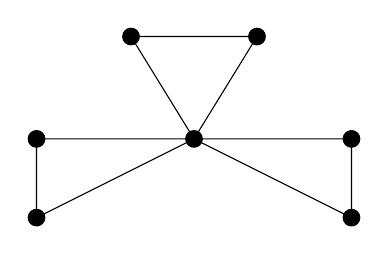
\begin{tikzpicture}
\coordinate (2x) at (0,0);
\coordinate (2) at (-2,0);
\coordinate (3x) at (2,0);
\coordinate (2x+2) at (-2,-1);
\coordinate (x) at (2,-1);
\coordinate (2+x) at (-0.8,1.3);
\coordinate (3x+2) at (0.8,1.3);

\draw (2x)--(3x)--(x)--(2x)--(2x+2)--(2)--(2x)--(2+x)--(3x+2)--(2x);

\foreach \point in {2x,2,3x,2x+2,x,2+x,3x+2}
\draw[fill=black] (\point) circle (3pt);

\end{tikzpicture}

\qquad\qquad

%TIP2
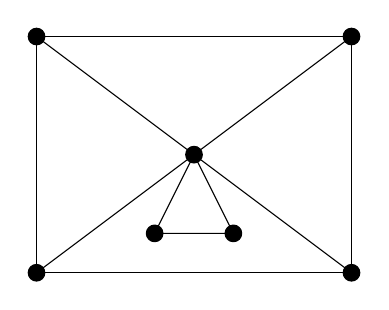
\begin{tikzpicture}
\coordinate (2) at (0,0);
\coordinate (y) at (-2,1.5);
\coordinate (2+x+y) at (2,1.5);
\coordinate (x+y) at (-2,-1.5);
\coordinate (2+y) at (2,-1.5);
\coordinate (x) at (-0.5,-1);
\coordinate (2+x) at (0.5,-1);

\draw (y)--(2+x+y)--(2+y)--(x+y)--(y);
\draw (x+y)--(2)--(y);
\draw (2+y)--(2)--(2+x+y);
\draw (2)--(x)--(2+x)--(2);

\foreach \point in {2,y,2+x+y,x+y,2+y,x,2+x}
\draw[fill=black] (\point) circle (3pt);

\end{tikzpicture}

}
\caption{Levo: graf tipa 1, desno: graf tipa 2}
\label{tip1,2}
\end{figure}

Dokažimo sedaj še obrat. Naj ima torej graf $\Gamma(R)$ prerezno vozlišče $a$. Denimo najprej, da $R$ ni lokalni kolobar. Potem po izreku 8.7 iz \cite{Atiyah} $R$ lahko zapišemo kot $R=R_1 \times \dots \times R_n$, kjer je $n\ge 2$ in so vsi $R_i$ končni lokalni kolobarji. Po posledici \ref{cutVertexOneNonzeroComponent} in  izreku \ref{cutVertexClassification} sledi, da je $a = (a_1,0,\dots,0)$, kjer velja ena od naslednjih možnosti
\begin{enumerate}
\item $a_1 = 1$ in $R_1\cong \Z_2$,
\item $R_1 \cong \Z_4$ in $a_1 = 2$ ali $R_1 \cong \Z_2[x] / (x^2)$ in $a_1 = x$,
\item $a_1$ je prerezno vozlišče v $\Gamma(R_1)$, ki ob odstranitvi izolira vsaj eno vozlišče.
\end{enumerate}
Opazimo, da v vsakem izmed zgornjih treh primerov lahko v $\Gamma(R)$ najdemo vozlišče stopnje 1 in sicer 
\begin{enumerate}
\item $(0,1,\dots,1)$,
\item $(2,1,\dots,1)$ ali $(x,1,\dots,1)$,
\item $(b,1,\dots,1)$, kjer je $b\in V(\Gamma(R_1))$ vozlišče stopnje ena,
\end{enumerate}
s čimer dokaz v primeru kolobarja, ki ni lokalen, lahko zaključimo. 

Predpostavimo sedaj, da je $R$ lokalni kolobar. Označimo z $m$ njegov edini maksimalni ideal in s $k$ najmanjše naravno število, da je $m^k = 0$. Iz leme \ref{localRingCutVertex} vemo, da je $m^{k-1} =  \{a,0\}$. Ker je poleg tega še $m = Z(R)$, to implicira, da je $a$ soseden z vsemi drugimi vozlišči $\Gamma(R)$ in da je $2a = 0$. Ker je $a$ prerezno vozlišče, po njegovi odstranitvi graf $\Gamma(R)$ razpade na $n\ge 2$ komponent. Označimo jih z $G_1,\dots, G_n$. Če je v eni izmed komponent eno samo vozlišče, smo našli vozlišče stopnje ena in smo s tem izrek dokazali. Predpostavimo torej, da ima vsaka komponenta $G_i$ vsaj dve vozlišči. Naj bo zdaj $i\neq j$ in $x\in G_i, y\in G_j$. Potem je $xy \neq 0$, ker sta iz različnih komponent in $xy \in Z(R)$, ker je $Z(R)$ v tem primeru ideal. Ker so komponente $G_k$ po predpostavki povezane in imajo vsaj dve vozlišči, obstajata $s\in G_i\setminus\{x\}$  za katerega velja $sx = 0$ in $t\in G_j \setminus \{y\}$, za katerega velja $ty = 0$. Potem je $s-xy -t$ pot med $s$ in $t$ v $\Gamma(R)$ (to velja tudi, če je $xy = s$ ali $xy = t$). To pa implicira, da je $xy = a$, saj sicer pridemo v nasprotje s tem, da je $a$ prerezno vozlišče. Sklenemo torej, da za poljubna $i\neq j$ in za poljubna $x\in G_i, y\in G_j$ velja $xy = a$.

Naj bo zdaj $y\in G_j$ in $t\in G_j\setminus{y}$ tak, da je $ty=0$. Potem je za vsak $k\in \N$ tudi $ty^k = 0$. Potem je $y^k \in G_j \cup\{0,a\}$, saj je $t$ povezan le z elementi iz $G_j \cup \{a\}$. Naj bo zdaj $i \neq j  $ in $x\in G_i$. Potem je po zgoraj ugotovljenem $xy=a$ in zato $xy^2 = ay = 0$. Če je $y^2 \in G_j$ smo prišli do protislovja s tem, da sta $G_i $ in $G_j$ različni komponenti. Sledi torej, da je $y^2  \in \{0,a\}$. Denimo, da je $y^2 = a$. Potem je $y^3 = y^2 y = ay = 0$. Sledi, da je za vsak $z\in Z(R)$ $z^3 = 0$. Poleg tega je še $y(y-x) = y^2 - xy = a -a = 0$ in je zato $y-x \in V(G_j)$. Od tod sledi še $a = x(y-x) = xy - x^2 = a - x^2$ in zato je $x^2 = 0$ za vsak $x\in G_i, i\neq j$. Ugotovili smo torej, da je $z^2 = 0$ za vsak $z\in Z(R)$ ali pa obstaja natanko ena komponenta $G_j$ (predpostavimo lahko, da je to $G_1$), da je $y^3 = 0$ za vsak $y\in G_1$ in za vsak $i\neq 1$ je $x^2 = 0$ za vsak $x\in G_i$. Poleg tega vemo že, da je $2a = 0$. Od tod sledi, da bo karakteristika $R$ sodo število. Ker pa je $R$ lokalni kolobar, bo karakteristika  $R$ oblike $2^k, k \ge 1$. Če je $k > 1$, potem je $2\in Z(R)$ in mora torej veljati bodisi $2^2 = 0$ bodisi $2^3 = 0$. Zaključimo, da je karakteristika $R$ enaka 2,4 ali 8. Prav tako iz zgornjega sledi še, da je v primeru, ko je karakteristika enaka 8, element $a$ enak $a = 2^2 = 4$ (za 2 namreč velja, da je $2^2 \neq 0$).

Naj bo spet $y\in G_1$ in $t\in   G_1 \setminus \{y\}$ tak element, da zanj velja $yt = 0$. Naj bo še $i \neq 1$ in $x\in G_i$. Denimo, da je $|G_i|  \ge 3$. Poglejmo si element $x+a$. Velja $x(x+a) = x^2 + xa = 0+ 0 = 0$, torej mora biti $x+a\in G_i$. Vzemimo sedaj poljuben element $z\in G_i$, ki je soseden z $x+a$. Potem je $0=z(x+a) =zx + za =zx$ in zato je $z$ povezan tudi z $x$. Ker je $G_i$ povezana in ima vsaj tri vozlišča, obstaja $v\in G_i \setminus \{x,x+a\}$, ki zadošča $xv = 0$. Potem je $x(x+v) = x^2 + xv = 0 + 0 = 0$ in $y(x+v) = yx +yv = a + a = 2a = 0$. Sledi, da je element $x+v$ bodisi enak 0 bodisi $a$, saj je sicer povezan z elementom iz $G_1$ in z elementom iz $G_i$, kar je v nasprotju z definicijo komponent za povezanost.
Denimo najprej, da je karakteristika $R$ enaka 2 ali da je $2x=0$. Če je $x+v=0$, potem je $v=-x=x$, kar je v nasprotju z izbiro $v$ (zadnja enakost sledi, ker je $x=-x$). Podobno je v primeru, ko je $x+v = a$, $v = a-x = a + x$, kar je spet v nasprotju z izbiro $v$. Denimo torej, da je $2x\neq 0$. Velja $(2x)x = 2x^2  = 0$, torej je $2x \in G_i \cup\{a\}$. Ker pa je še $(2x)y = 2 (xy) = 0$, mora biti $2x = a$. Če je zdaj še $x+v = a = 2x$, je $v=x$, kar je v nasprotju z izbiro $v$. Sledi, da mora biti $x+v=0$ oziroma $v=-x$. Če je karakteristika $R$ enaka 4, je $v = - x = 3x = x+ 2x = x+a$. Protislovje. Denimo torej, da je karakteristika $R$ enaka 8. Po predpostavki je $v \neq x+a = x+2x = 3x$. Od tod pa sledi, da je $x+v \neq x+3x = 4x = ax = 0$. Protislovje z zgornjo predpostavko. Sklenemo, da mora  za vsak $i\neq1$ veljati $|G_i| = 2$.

Sedaj ločimo dva primera. Denimo najprej, da obstaja $y\in G_1$, ki zadošča $y^2 \neq 0$. Po zgoraj ugotovljenem mora potem veljati $y^2 = a $ in $y^3 = 0$. Naj bo zdaj $x\in G_2$. Potem je $y(x+y) = xy + y^2 = a +a = 2a = 0$, torej je $x+y\in G_1$. Denimo najprej, da je $n\ge 3$, torej imamo po odstranitvi elementa $a$ vsaj tri komponente za povezanot. Naj bo $z\in G_3$. Potem je $z(x+y) = zx + zy = a+ a= 2a = 0$. Sledi, da mora biti $z\in G_1$, kar je v nasprotju z izbiro elementa $z$. Zaključimo, da mora biti $n=2$. To pa pomeni, da je $V(\Gamma(R)) = V(G_1) \cup V(G_2) \cup \{a\}$. Poleg tega smo zgoraj že ugotovili, da je $|G_2| = 2$  in ker je $x(x+a) = x^2 + xa = 0+0= 0$, je $G_2 = \{x,x+a\}$. Podobno se enostavno prepričamo, da je $\{y,x+y,y+a,x+y+a\}\subseteq G_1$. 

Recimo, da je $|G_1| \ge 5$. Potem enako kot zgoraj vidimo, da obstaja $s\in G_1 \setminus \{y,x+y,y+a,x+y+a\}$, ki zadošča bodisi $sy = 0$ bodisi $s(x+y)=0$. Poglejmo si najprej drugi primer, ko je $s(x+y) = 0$. Potem je $0 = s(x+y) = sx + sy = a + sy$. Ker je $2a = 0$, je $a=sy$. Poleg tega $x(s+y) = xs +xy = a + a = 2a = 0$ in $y(y+s) = y^2 + ys = a + a = 2a = 0$. Sledi, da mora biti $y+s$ bodisi $0$ bodisi $a$, saj sicer pridemo v nasprotje z razcepom na komponente. Sedaj naredimo analogen premislek kot zgoraj. Če je karakteristika $R$ enaka 2 ali je $2y = 0$, potem iz $s+y=0$ dobimo $s=y$ in iz $s+y = a$ dobimo $s = y+a$. Protislovje v obeh primerih. Denimo torej, da $2y\neq 0$. Ker je $(2y)x = 2 (xy) = 2a=0$ in $2y(x+y) = 2(xy + y^2 ) = 2 (a+ a) = 0$, mora biti $2y = a$. Če je $y+s = a = 2y $, je $s = y$. Protislovje. Če je $y+s = 0$ in je $R$ karakteristike 4, je $s = -y = 3y = y +2y = y+a$. Protislovje. Če pa je $y+s = 0$ in je $R$ karakteristika $R$ enaka 8, iz zveze $s \neq y+a = y+ 2y = 3y$ dobimo $y+s \neq 4y = ay =0$. Protislovje. Sklenemo, da ne more veljati $s(x+y) = 0$.

Poglejmo si sedaj primer, ko je $sy = 0$. Potem je $y(x+y+s) = yx + y^2 + ys = a + a + 0= 2a = 0$ in $x(x+y+s) = x^2 + xy + xs = 0 + a + a = 2a = 0$. Sledi, da mora biti $x+y+s\in \{0,a\}$. Analogno kot v prvem primeru pokažemo, da se to ne more zgoditi. V vseh primerih torej pridemo do protislovja, zato mora biti $|G_1| = 4$. Sledi, da je $G_1 = \{y,x+y,y+a,x+y+a\}$. Pri tem je $y$ povezan z elementi iz množice $\{x+y,x+y+a,a\}$, $x+y$ je povezan z elementi iz $\{y,y+a,a\}$, $y+a$ je povezan z elementi iz $\{x+y,x+y+a,a\}$, $x+y+a$ pa je povezan z elementi iz $\{y,y+a,a\}$. Iz pravkar povedanega in iz zgoraj dokazanega sledi, da je graf $\Gamma(R)$ ravno graf tipa 2 s slike \ref{tip1,2} (pri tem je $x+a\in G_2$ povezan z $a$, ker je $a^2 = 0$, kar sledi iz tega, da je $m^{k-1}=\{0,a\}$ in $m^k=0$). V \cite{Redmond} so bili natančno določeni kolobarji, ki imajo tak graf deliteljev niča. Izkaže se, da mora biti $R$ izomorfen enemu od kolobarjev $\Z_4[x]/(x^2 + 2x), \Z_8[x]/(2x, x^2 + 4), \Z_2[x,y]/(x^2,y^2 - xy), \Z_4[x,y]/(x^2,y^2 - xy, xy-2,2x,2y)$.

Ostane nam torej le še primer, ko za vsak $x\in Z(R)$ velja $x^2 = 0$. Vemo že, da je $V(\Gamma(R)) = V(G_1) \cup V(G_2) \cup \dots \cup V(G_n) \cup \{a\}$, kjer ima vsaka komponenta $G_i$ dve vozlišči. Označimo $V(G_i) = \{x_i,x_i +a  \}$. Denimo najprej, da je $n\ge 4$. Naj bo $y\in G_1$ in $ x\in G_2$. Potem velja $x+y\notin G_1 \cup G_2 \cup \{a\}$. Denimo nasprotno, da je $x+y \in G_1$. Če je $x+y  = y$, je $x=0$, kar je v nasprotju z definicijo grafa deliteljev niča. Če pa je $x+y = y+a$, je $x=a$, kar je spet v nasprotju s tem, da je $G_2 = \{x,x+a\}$. Analogno vidimo, da $x+y\notin G_2$. Če pa je $x+y=a$, je $0 = xa = x(x+y) = x^2 + xy = 0+a = a$. Protislovje. Predpostavimo torej lahko, da je $x+y\in G_3$. Naj bo še $z\in G_4$. Potem je $z(x+y) = zx + zy = a +a = 2a = 0$, torej mora biti še $z\in G_3$. Protislovje. Sledi, da je $n\le 3$. Vemo, da $n\neq 1$, sicer $a$ nebi bilo prerezno vozlišče. Če je $n=2$, potem ima $\Gamma(R)$ 5 vozlišč. V \cite{Redmond} so klasificirani vsi grafi deliteljev niča na 5 vozliščih, vendar noben izmed njih nima željene oblike (noben nima prereznega vozlišča za katerega velja, da ob njegovi odstranitvi dobimo dva grafa $K_2$). Zaključimo, da mora biti $n=  3$ in $V( \Gamma(R)) = V(G_1) \cup V(G_2) \cup V(G_3) \cup \{a\}$. Pri tem imajo vse tri komponente $G_i$ po dve vozlišči. Zaklučimo torej, da je graf $\Gamma(R)$ ravno graf tipa 1 s slike \ref{tip1,2}. V \cite{Redmond} je dokazano, da je potem $R$ izomorfen enemu izmed kolobarjev $\Z_4[x,y]/(x^2,y^2,xy-2,2x,2y), \Z_2[x,y]/(x^2,y^2),\Z_4[x]/(x^2)$. S tem je ta izrek dokazan.


\endproof

%VOZLIŠČA STOPNJE 1
\section{Vozlišča stopnje 1}

\begin{lema}
\label{vertexOfDegree1}
Naj bo $R$ končni komutativni enotski kolobar, ki ni izomorfen $\Z_4$ ali $\Z_2[x]/(x^2)$. Graf $\Gamma(R)$ ima vozlišče stopnje 1 natanko tedaj, ko je bodisi $R$ izomorfen $\Z_9$ ali $\Z_3[x]/(x^2)$ bodisi v $R$ obstaja element $x$, za katerega velja $|\ann_R(x) | = 2$.
\end{lema}

\proof
Če je $R$ izomorfen $\Z_9$ ali $\Z_3[x]/(x^2)$, potem je graf $\Gamma(R)$ izomorfen $K_2$. Ta očitno ima vozlišče stopnje 1. Naj bo zdaj $R$ tak, da obstaja element $x$, za katerega velja, da je $|\ann_R(x)| = 2$. To pomeni, da je poleg 0 v $\ann_R(x)$ še en neničelen element. Če je ta različen od $x$, potem ima $x$ enega samega soseda in je zato  $\deg(x) = 1$. Če pa je $\ann_R(x) = \{0,x\}$, potem mora biti zaradi povezanosti grafa $\Gamma(R)$ ta enak kar grafu $K_1$, kar pomeni, da imamo eno samo vozlišče in nobene povezave. Po \cite{Anderson-klasifikacijaMalihGrafov} je v tem primeru $R$ izomorfen kolobarju $\Z_4$ ali $\Z_2[x]/(x^2)$, kar pa je v nasprotju s predpostavko leme.

Dokažimo še obrat. Denimo, da ima $\Gamma(R)$ vozlišče $x$, ki zadošča $\deg(x)=1$. Naj ima najprej $\Gamma(R)$ le dve vozlišči. Potem je $\Gamma(R)$ izomorfen grafu $K_2$. Po \cite{Anderson-klasifikacijaMalihGrafov} je potem $R$ izomorfen enemu izmed kolobarjev $\Z_9, \Z_2 \times \Z_2, \Z_3[x]/(x^2)$. Opazimo, da je $\ann_{\Z_2 \times \Z_2}((1,0)) = \{(0,0), (0,1)\}$, torej je $|\ann_{\Z_2 \times \Z_2}((1,0))| = 2$. Podobno je $|\ann_{\Z_2 \times \Z_2}((0,1))| = 2$. 
Poglejmo si še primer, ko ima $\Gamma(R)$ vsaj tri vozlišča. Potem je jasno, da je edini sosed vozlišča $x$ prerezno vozlišče. Označimo ga z $a$. Velja bodisi $\ann_R(x) = \{0,a\}$ bodisi $\ann_R(x) = \{0,a,x\}$. V drugem primeru je potem $x^2 = 0$. Od tod sledi, da je $x(x+a) = x^2 + xa = 0 + 0 = 0$ in zato je $x+a \in \ann_R(x) = \{0,a,x\}$. Če je $x+a = x$, je $a=0$. Protislovje. Podobno dobimo, da $x+a\neq a$. Sledi torej, da je $x+a=0$ oziroma $x=-a$. Ker pa je vsak sosed vozlišča $a$ tudi sosed vozlišča $-a=x$, mora biti $\Gamma(R)$ izomorfen grafu $K_2$ (ker $x$ soseden le z $a$). To pa je v nasprotju s tem, da ima graf vsaj tri vozlišča.
\endproof

Združimo to lemo z ugotovitvami prejšnjega razdelka.

\begin{posledica}
Naj bo $R$ tak končni komutativni enotski kolobar, da ima $\Gamma(R)$ vsaj tri vozlišča. Graf $\Gamma(R)$ ima prerezno vozlišče natanko tedaj, ko je izpolnjen eden izmed naslednjih dveh pogojev
\begin{enumerate}
\item obstaja $x\in R$, da je $|\ann_R(x)| = 2$ ali
\item $R$ je izomorfen enemu izmed naslednjih sedmih kolobarjev: $\Z_4[x,y]/(x^2, y^2, \\xy-2,2x,2y), \Z_2[x,y]/(x^2,y^2), \Z_4[x]/(x^2),  \Z_4[x]/ (x^2+2x), \Z_8[x]/(2x,x^2 + 4), \Z_2[x,y]/(x^2, y^2 - xy), \Z_4[x,y]/(x^2, y^2 - xy, xy-2,2x,2y)$.
\end{enumerate}
\end{posledica}

\proof
Sledi direktno iz izreka \ref{izrek-cutVertex} in leme \ref{vertexOfDegree1}.
\endproof

\begin{lema}
Naj bo $R$ končni komutativni enotski kolobar. Prerezna vozlišča grafa $\Gamma(R)$ tvorijo poln podgraf grafa $\Gamma(R)$.
\end{lema}

\proof
Smiselno je gledati le kolobarje, katerih grafi imajo vsaj dve prerezni vozlišči. Pripomnimo, da imajo po lemi \ref{localRingCutVertex} lokalni kolobarji kvečjemu eno prerezno vozlišče in zato za njih trditev očitno velja.

Naj bo torej $R$ tak kolobar, da ima graf $\Gamma(R)$ vsaj dve prerezni vozlišči. Označimo ju z $a$ in $b$. Potem graf $\Gamma(R)$ ob odstranitvi vozlišča $a$ razpade na dva disjunktna podgrafa $G_1$ in $G_2$. Predpostavimo lahko, da je $b\in G_2$. Naj bo $x_a\in G_1$ sosed vozlišča $a$ v $\Gamma(R)$. Analogno graf $\Gamma(R)$ ob odstranitvi vozlišča $b$ razapde na dva disjunktna podgrafa $H_1$ in $H_2$. Spet lahko predpostavimo, da je $a\in H_2$ in izberemo $x_b\in H_1$, ki je soseden z $a$ v $\Gamma(R)$. Poglejmo si zdaj najkrajšo pot med $x_a$ in $x_b$ v $\Gamma(R)$. Če ta pot ne vsebuje vozlišča $a$, jo lahko podaljšamo s povezavo $x_b-b$ in tako dobimo pot med $x_a$ in $b$, ki ne obišče vozlišča $a$. To je v nasprotju s tem, da je $a$ prerezno vozlišče in da sta podgrafa $G_1$ in $G_2$ disjunktna. Podobno vidimo  še, da mora ta pot vsebovati tudi vozlišče $b$. Sklenemo torej, da sta tako $a$ kot $b$ na najkrajši poti med vozliščema $x_a$ in $x_b$. Po \cite{diploma} je $\dist(x_a,x_b)\le 3$, zato mora biti najkrajša pot med njima oblike $x_a  -  a - b - x_b$. To pa pomeni, da morata biti $a$ in $b$ povezana. Ker sta bili prerezni vozlišči poljubni, sledi da prerezna vozlišča tvorijo poln podgraf.
\endproof

\begin{lema}
Naj bo $R$ končni komutativni enotski kolobar. Označimo z $N$ število prereznih vozlišč grafa $\Gamma(R)$. Velja $0\le N \le |V(\Gamma(R))|/2$.
\end{lema}

\proof
Jasno je, da je $N\ge 0$. Poleg tega obstajajo grafi deliteljev niča, ki nimajo prereznih vozlišč. Vzamemo lahko npr $R=\F_m \times \F_n$, kjer je $\F_i$ polje z $i$ elementi in sta $m,n \ge 3$. Velja namreč $\Gamma(\F_m \times \F_n) = K_{m-1,n-1}$. Prav tako obstaja kolobar, pri katerem je dosežena zgornja meja iz izreka. Res, vzemimo $R=\Z_2 \times \Z_2 \times \Z_2$. Graf $\Gamma(R)$ je tak kot $K_3$, le da ima iz vsakega vozlišča še eno povezavo. V tem primeru je torej $|V(\Gamma(R))| = 6$, poleg tega pa ima tri prerezna vozlišča. Preveriti je torej potrebno le še, da za vsak graf deliteljev niča res velja zgornja meja iz izreka. Predpostavimo torej, da je $R$ tak, da ima prerezno vozlišče. Potem je po \ref{izrek-cutVertex} kolobar $R$ bodisi izomorfen enemu izmed sedmih v izreku naštetih kolobarjev bodisi ima $\Gamma(R)$ vozlišče stopnje 1. Vemo že, da ima vsak od sedmih omenjenih kolobarjev bodisi graf tipa 1 bodisi graf tipa 2 s slike \ref{tip1,2}. Potem ima očitno sedem vozlišč in le eno prerezno vozlišče in zadošča oceni iz leme. Prav tako vemo, da imajo grafi deliteljev niča lokalnih kolobarjev kvečjemu eno prerezno vozlišče in tudi zanje trditev očitno velja. Naj bo torej $R$ kolobar, ki ni izomorfen nobenemu od sedmih kolobarjev iz izreka \ref{izrek-cutVertex} in ki ni lokalen. Iz izreka \ref{cutVertexClassification} sledi, da vsako prerezno vozlišče ob odstranitvi izolira vsaj eno vozlišče. To pa pomeni, da za vsako prerezno vozlišče obstaja vsaj eno vozlišče stopnje 1. Od tod sledi $2N \le |V(\Gamma(R)) |$ oziroma $N \le |V(\Gamma(R))| /2$.
\endproof

% KVOCIENT STEVILA MAKSIMALNIH VOZLIŠČ IN STEVILA VOZLISC
\begin{primer}
Definirajmo $V_{\max} (\Gamma(R)) = \{v\in v(\Gamma(R)); v \textrm{ maksimalne stopnje}\}$. Poglejmo si, kakšne vrednosti lahko zavzame izraz 
$$
\frac{|V_{\max}(\Gamma(R))|}{|V(\Gamma(R)|}.
$$
Naj bo najprej $R$ polkolobar oblike $R \cong R_1 \times R_2$, kjer sta $R_1$ in $R_2$ poljubna cela polkolobarja moči $|R_1| = n$ in $|R_2| = m$, $m \le n$. Taka polkolobarja $R_1$ in $R_2$ seveda obstajata, vzamemo lahko kar linearno urejeni množici moči $n$ in $m$. Jasno je, da je $\Gamma(R) \cong K_{n-1,m-1}$. Od tod sledi, da je $\frac{|V_{\max}(\Gamma(R))|}{|V(\Gamma(R)|} = \frac{m-1}{n+m-2}$. 

Poglejmo si sedaj množico števil $\{\frac{a}{b}; \textrm{ obstaja polkolobar } R \textrm{, da je } |V_{\max}(\Gamma(R))| = a \textrm{ in } |V(\Gamma(R))| = b \}$. Po zgornjem premisleku je ta množica števil gosta podmnožica v $[0, \frac{1}{2}]\cap\Q$ in posledično seveda tudi v $[0,\frac{1}{2}]$.

Omejimo se sedaj na komutativne kolobarje z enoto in opazujmo isti kvocient kot zgoraj. Naj bo $R\cong \GF(p^k) \times \GF(q^l)$. Jasno je, da je $\Gamma(R) \cong K_{p^k - 1, q^l -1}$. Predpostavimo sedaj, da je $p^k \le q^l$. Potem je $\frac{|V_{\max}(\Gamma(R))|}{|V(\Gamma(R)|} = \frac{p^k - 1}{p^k + q^l -2}$. Od tu spet sledi, da je opazovani kvocient lahko enak poljubnemu številu iz množice
$$
\Big\{\frac{p^k - 1}{p^k + q^l -2}; p,q \textrm{ praštevili }, k,l \in \N, p^k \le q^l\Big\}.
$$
\end{primer}

% URAVNOTEŽENI GRAFI MATRIČNIH KOLOBARJEV
\section{Uravnoteženi grafi deliteljev niča matričnih kolobarjev}

Zgoraj smo že definirali usmerjeni graf deliteljev niča $\Gamma_d(R)$. Definirajmo sedaj še nekaj pojmov, povezanih z vozlišči grafa. Naj bo $a\in V(\Gamma_d(R))$ poljubno vozlišče. Število povezav oblike $x\rightarrow a$ imenujemo \emph{notranja stopnja} vozlišča $a$, število povezav oblike $a\rightarrow x$ pa \emph{zunanja stopnja} vozlišča $a$. Če graf ni usmerjen, je jasno, da oba pravkar definirana pojma sovpadata s stopnjo vozlišča. Pravimo še, da je graf \emph{uravnotežen}, če za vsako vozlišče grafa njegova notranja in zunanja stopnja sovpadata.

Če je kolobar $R$ končen, z lahkoto določimo notranjo in zunanjo stopnjo poljubnega vozlišča. Naj bo torej $a$ vozlišče grafa $\Gamma_d(R)$. Potem je notranja stopnja $a$ enaka $|l_R(a)|-1$, če $a^2 \neq 0$ in $|l_R(a)|-2$, če $a^2 = 0$. Podobno je zunanja stopnja $a$ enaka $|r_R(a)|-1$, če $a^2 \neq 0$ in $|r_R(a)| - 2$, če $a^2 = 0$.

\begin{izrek}
\label{inDegreeOutDegree}
Naj bo kolobar $R$ komutativni končni glavni kolobar z enoto. Naj bo $n \ge 2$. Naj bo $A\in \M_n(R)$ neničelni delitelj niča in naj bodo $d_1,d_2, \dots,d_n$ osnovni delitelji matrike $A$. Potem sta tako notranja kot zunanja stopnja vozlišča $A$ v $\Gamma_d(\M_n(R))$ enaki
$$
\prod_{i=1}^n |\ann_R(d_i)|^n - \epsilon,
$$ 
stopnja vozlišča $A$ v $\Gamma(\M_n(R))$ pa je enaka
$$
2\prod_{i=1}^n |\ann_R(d_i)|^n - \prod_{i,j=1}^n |\ann_R(d_i) \cap \ann_R(d_j)| - \epsilon,
$$
kjer je $\epsilon =1$, razen v primeru, ko je $A^2 = 0$. Tedaj je $\epsilon = 2$. Zgornja ugotovitev o notranji in zunanji stopnji implicira še, da je graf uravnotežen.
\end{izrek}
 
\proof
Po izreku  \ref{PIR-elementaryDivisionRing} vemo, da je vsak komutativni glavni kolobar z enoto osnovni kolobar z deljenjem. To pa pomeni, da je matrika $A$ ekvivalentna matriki $D_A= \text{diag}(d_1,\dots,d_n)$. Iz leme \ref{anihilatorProduktZObrnljivim} sledi, da je $|l_{\M_n(R)}(A)| = |l_{\M_N(R)}(D_A)|$ in $|r_{\M_N(R)}(A)| = |r_{\M_N(R)}(D_A)|$. Naj bo zdaj $X=(x_{ij})_{i,j=1}^n\in \M_N(R)$ poljubna matrika. Potem velja, da je $XD_A = 0$ natanko tedaj, ko je $x_{ij}d_j = 0$ za $i,j = 1, \dots, n$. Podobno je $D_AX = 0$ natanko tedaj, ko je $d_i x_{ij} =0 $ za $i,j=1,\dots,n$. Sledi, da je 
$$
|l_{\M_n(R)}(D_A)| = \prod_{i=1}^n |\ann_R(d_i)|^n = |r_{\M_n(R)}(D_A)|
$$
in posledično je po zgoraj ugotovljenem
$$
|l_{\M_n(R)}(A)|= |r_{\M_n(R)}(A)| = \prod_{i=1}^n |\ann_R(d_i)|^n .
$$
Če se spomnimo ugotovitve z začetka razdelka, lahko zaključimo, da sta notranja in zunanja stopnja res obe enaki $\prod_{i=1}^n  |\ann_R(d_i)|^n - \epsilon$, kjer je $\epsilon = 1$ (iz množice deliteljev niča odstranimo ničelno matriko), razen v primeru, ko je $A^2 = 0$ in je $\epsilon = 2$ (matrika ni povezana sama s sabo). 

Iz zgornjih zvez sledi še, da je matrika $X\in l_{\M_n(R)}(D_A)\cap r_{\M_n(R)}(D_A)$ natanko tedaj, ko je $x_{ij} \in  \ann_R(d_i)\cap \ann_R(d_j)$. Posledično je 
$$
|l_{\M_n(R)}(A) \cap r_{\M_n(R)}(A)| = \prod_{i,j=1}^n | \ann_R(d_i) \cap \ann_R(d_j)|.
$$
Ugotovitve sedaj združimo v 
$$
|l_{\M_n(R)}(A) \cup r_{\M_n(R)}(A)| = |l_{\M_n(R)}(A)|  + |r_{\M_n(R)}(A)| - |l_{\M_n(R)}(A) \cap r_{\M_n(R)}(A)|=
$$
$$
2\prod_{i=1}^n |\ann_R(d_i)|^n - \prod_{i,j=1}^n |\ann_R(d_i) \cap \ann_R(d_j)|.
$$
Sklenemo, da je stopnja vozlišča $A$ v grafu $\Gamma(\M_n(R))$ res enaka $2\prod_{i=1}^n |\ann_R(d_i)|^n - \prod_{i,j=1}^n |\ann_R(d_i) \cap \ann_R(d_j)| -\epsilon$, kjer je $\epsilon=1$, razen v primeru, ko je $A^2 = 0$. Takrat je $\epsilon=2$.
\endproof

\begin{primer}
Denimo, da je kolobar $R$ polje $R=\GF(p^{\alpha})$. Vzemimo poljubno matriko $A\in \M_n(\GF(p^{\alpha}))$ kot zgoraj v izreku. Potem lahko zgornje formule nekoliko poenostavimo. Res, poljubni osnovni delitelj je namreč bodisi obrnljiv bodisi je 0. Velja še, da je število neničelnih osnovnih deliteljev matrike $A$ enako njenemu rangu. Velja $\ann_R(d_i) = 0$, če je $d_i$ obrnljiv element in $\ann_R(d_i) = R=\GF(p^{\alpha})$, če je $d_i=0$. Označimo s $k$ rang matrike $A$ (ker $A$ ni obrnljiva, je $k<n$). Potem velja 
$$
|l_{\M_n(R)}(A)| = |r_{\M_n(R)}(A)|=\prod_{i=1}^n|\ann_R(d_i)|^n = \prod_{i=1}^k |\{0\}|^n\cdot \prod_{i=k+1}^n |R|^{n} =|\GF(p^{\alpha})|^{n(n-k)}
$$
in
$$
|l_{\M_n(R)} (A) \cup r_{\M_n(R)}(A)| = 2|\GF(p^{\alpha})|^{n(n-k)} - |\GF(p^{\alpha})|^{(n-k)^2}.
$$
Sledi, da sta notranja in zunanja stopnja matrike $A\in \M_n(\GF(p^{\alpha}))$ v usmerjenem grafu $\Gamma_d(\M_n(\GF(p^{\alpha})))$ enaki 
$$
|\GF(p^{\alpha})|^{n(n-k)} - \epsilon,
$$
stopnja $A$ v $\Gamma (\M_n(\GF(p^{\alpha})))$ pa je enaka
$$
 2|\GF(p^{\alpha})|^{n(n-k)} - |\GF(p^{\alpha})|^{(n-k)^2} - \epsilon,
$$
kjer je $\epsilon=1$, če $A^2\neq 0$ in $\epsilon = 2$, če je $A^2 = 0$. 
\end{primer}

Zgornji izrek lahko sedaj uporabimo pri dokazu naslednjega izreka. Pred tem pa moramo razviti še malo teorije. Če za zaporedje različnih povezav $e_1, \dots, e_s$ v usmerjenem grafu velja, da je končno vozlišče povezave $e_i$ enako začetnemu vozlišču povezave $e_{i+1}$ za vsak $1 \le i \le s-1$ in če je še končno vozlišče $e_s$ enako začetnemu vozlišču povezave $e_1$, potem pravimo da je zaporedje vozlišč $e_1,\dots,e_s$ \emph{cikel} v usmerjenem grafu. Enako kot za neusmerjene grafe definiramo, da je cikel \emph{Eulerjev cikel}, če vsebuje vsako povezavo natančno enkrat (in obišče vsako vozlišče, kar je ekvivalentno zahtevi, da je graf povezan). Graf oziroma usmerjen graf je Eulerjev, če vsebuje Eulerjev cikel.

Dokažimo naslednjo lemo, ki povezuje Eulerjeve in uravnotežene grafe.
\begin{lema}
\label{usmerjenGrafEuler}
Usmerjen graf je Eulerjev natanko tedaj, ko je povezan in uravnotežen.
\end{lema}

\proof
Naj bo graf Eulerjev. Potem mora biti očitno povezan. Ker Eulerjev cikel vsakič, ko obišče neko vozlišče vanj vstopi in izstopi po drugi povezavi, mora biti število vstopnih povezav enako številu izstopnih povezav. Povedano drugače, notranja in zunanja stopnja vsakega vozlišča se morata ujemati, torej mora biti graf uravnotežen.

Naj bo zdaj usmerjen graf $G$ povezan in uravnotežen. Z indukcijo na število povezav grafa pokažimo, da mora biti graf Eulerjev. Če je moč množice povezav $|E|=2$, potem imamo graf na dveh točkah $a,b$ s povezavama $a\rightarrow b$ in $b\rightarrow a$. Graf je Eulerjev. Oglejmo si sedaj povezan uravnotežen graf $G$ z $|E|> 2$ povezavami. Izberimo poljubno vozlišče $u$ in začnimo graditi pot, ki gre po vsaki povezavi največ enkrat. To storimo tako, da si v vsakem vozlišču preprosto izberemo povezavo po kateri še nismo potovali in gremo po njej do naslednjega vozlišča. Ko pridemo do vozlišča iz katerega ne moremo več nadaljevati poti, ker smo vse povezave že obhodili, mora biti to zaradi uravnoteženosti kar začetno vozlišče $u$. Denimo, da pri tem nismo obhodili vseh povezav grafa $G$. Oglejmo si graf $G'$, ki ga dobimo tako, da grafu $G$ odstranimo vse povezave na prej skonstruiranem ciklu in vsa izolirana vozlišča. Graf $G'$ ni nujno povezan, še vedno pa je uravnotežen, saj smo iz vsakega vozlišča odstranilo enako vhodnih in izhodnih povezav. Po indukcijski predpostavki vsaka povezana komponenta grafa $G'$ vsebuje Eulerjev cikel. Ker pa je graf $G$ povezan, mora zgoraj konstruirani cikel sekati vsako povezano komponento grafa $G'$ vsaj v eni točki. V vsaki povezani komponenti grafa $G'$ si torej izberemo eno vozlišče v katerem konstruirani cikel seka to komponento in v njem združimo konstrirani cikel in Eulerjev cikel te komponente. Dobimo Eulerjev cikel za $G$.
\endproof

\begin{lema}
Usmerjeni graf deliteljev niča $\Gamma_d(R)$ je povezan natanko tedaj, ko je množica levih deliteljev niča $Z_l(R)$ enaka množici desnih deliteljev niča $Z_r(R)$. Poleg tega v primeru, ko je $\Gamma_d(R)$ povezan, med poljubnima vozliščema $x$ in $y$ obstaja usmerjena pot dolžine največ tri.
\end{lema}

\proof

\endproof

\begin{izrek}
Naj bo $R$ končni komutativni glavni kolobar z enoto in $n\ge 2$. Tedaj je usmerjeni graf deliteljev niča $\Gamma_d(\M_n(R))$ Eulerjev.
\end{izrek}

\proof
POPRAVITI
Po lemi \ref{enostranskiDelitelji0Matricni} vemo, da sta v matričnih kolobarjih množici levih  in desnih deliteljev niča enaki. To implicira, da je usmerjeni graf povezan. Denimo nasprotno, da ni povezan. To pomeni, da obstajata dve vozlišči $x$ in $y$, da med njima ne morema najti poti v obe smeri. Predpostavimo lahko, da ne moremo najti poti od $x$ do $y$. 


To implicira, da v grafu obstaja vozlišče, ki je desni delitelj niča, ni pa levi delitelj niča, saj se vsaka pot, ki se začne v $x$ konča preden pride v $y$. To pa je v nasprotju s predpostavko o tem, da so levi in desni delitelji niča enaki. Sklenemo torej, da je $\Gamma_d(\M_n(R))$ povezan graf. Po izreku \ref{inDegreeOutDegree} je $\Gamma_d(\M_n(R))$ uravnotežen in zato po lemi \ref{usmerjenGrafEuler} Eulerjev.
\endproof

Poiščimo še primer komutativnega enotskega kolobarja $R$, da $\Gamma_d(\M_n(R))$ ne bo uravnotežen.

\begin{izrek}
Naj bo $R$ komutativni enotski kolobar in $n\ge2$. Če usmerjeni graf deliteljev niča $\Gamma_d(\M_n(R))$ ni uravnotežen, potem je $|R| \ge 8$. Poleg tega je ta ocena optimalna, saj obstaja komutativni enotski kolobar $R$ moči $|R|=8$, da $\Gamma_d(\M_n(R))$ ni uravnotežen. 
\end{izrek} 

\proof
Označimo z $\gamma(n)$ število neizomorfnih kolobarjev moči $n$. Pri tem upoštevamo tudi nekomutativne kolobarje in kolobarje brez enote. Vemo, da lahko vsak kolobar moči $n=p_1^{\alpha_1}\cdots p_r^{\alpha_r}$, kjer so $p_i$ paroma različna praštevila, razcepimo kot $R=R_1\times \dots \times R_r$, tako da je moč $|R_i| = p_i^{\alpha_i}$ (tak razcep dobimo iz razcepa Abelovih grup). Sledi, da je $\gamma$ multiplikativna, kar pomeni, da je $\gamma(n) = \gamma(p_1^{\alpha_1}\cdots p_r^{\alpha_r}) = \gamma(p_1^{\alpha_1})\cdots \gamma_(p_r^{\alpha_r})$. 

Sedaj opazimo, da je ničelni kolobar edini kolobar  z enim elementom. Jasno je tudi, da nima enote. Naj bo zdaj $R$ kolobar moči $p$, kjer je $p$ praštevilo. Po lemi \ref{pkolobar} je kolobar $R$ bodisi polje moči $p$ bodisi ničelni kolobar moči $p$. Sledi, da je $\gamma(p)= 2$. Pripomnimo še, da ničelni kolobar nima enote, graf $\Gamma_d(\M_n(\GF(p)))$ pa je uravnotežen po izreku \ref{inDegreeOutDegree}. 

Naj bosta zdaj $p\neq q$ različni praštevili. Zaradi multiplikativnosti $\gamma$ velja $\gamma(pq) = \gamma(p)\gamma(q) = 4$. Naj bo $R$ poljuben kolobar moči $pq$. Potem ima $R$ ideal $I_1$ moči $p$ in ideal $I_2$ moči $q$ in ker sta $p$ in $q$ različna, lahko zapišemo $R\cong I_1 \oplus I_2$. Če naj ima $R$ enoto, jo morata imeti tako $I_1$ kot $I_2$. Potem je $I_1\cong \GF(p)$ in $I_2\cong \GF(q)$. Ker je $\GF(p) \oplus \GF(q)$ glavni kolobar, poleg tega pa je tudi komutativen in ima enoto, je po \ref{inDegreeOutDegree} graf $\Gamma_d(\M_n(R))$ uravnotežen. 

Naj bo zdaj $|R|=p^2$, kjer je $p$ praštevilo. Znano je, da obstaja natanko 11 neizomorfnih kolobarjev moči $p^2$ (glej \cite{Fine}). Če je $R$ komutativni kolobar moči $p^2$ z enoto, potem je glavni. Res, naj bo $I$ poljuben pravi ideal. Potem mora imeti $I$ natanko $p$ elementov. Sledi, da je kot aditivna grupa generiran z neničelnim elementom, torej je $I$ glavni ideal. Po izreku \ref{inDegreeOutDegree} je graf $\Gamma_d(\M_n(R))$ spet uravnotežen.

Če označimo s $k=|R|$, potem je za $1<k<8$ število $k$ bodisi praštevilo bodisi produkt dveh različnih praštevil bodisi kvadrat praštevila. V vseh teh primerih pa smo zgoraj videli, da graf $\Gamma_d(\M_n(R))$ je uravnotežen. Če za nek kolobar $R$ graf $\Gamma_d(\M_n(R))$ ni uravnotežen, mora biti torej $|R|\ge 8$. Dokaz bo zaključen, če uspemo skonstruirati kolobar $R$  moči 8, da graf $\Gamma_d(\M_n(R))$ ne bo uravnotežen.

Označimo z $R$ $\Z_2$ algebro z bazo $\{1,a,b\}$ in z množenjem predpisanim takole
$$
\begin{array}{c | ccc}
\cdot & 1 & a & b \\
\hline
1 & 1 & a & b \\
a & a & 0 & 0 \\
b & b & 0 & 0 \\
\end{array}.
$$
Elementi $R$ so $R=\{0,1,a,b,1+a,1+b,a+b,1+a+b\}$ in $|R|=8$. Opazimo še, da $R$ ni glavni, saj ideal  $(a,b)$ generiran z elementoma $a,b$ ni glavni. Pokažimo sedaj, da $\Gamma_d(\M_2(R))$ ni uravnotežen graf. V ta namen bomo poračunali, da se vhodna  in izhodna stopnja vozlišča 
$A=
\begin{bmatrix}
a & 0 \\
b & 0 \\
\end{bmatrix}
$ ne ujemata.
Naj bo $B=
\begin{bmatrix}
x & y \\
z & w \\
\end{bmatrix}
$
poljubna druga matrika iz $\M_2(R)$. Določimo najprej vhodno stopnjo vozlišča $A$. Zanima nas torej, kdaj bo
$$
0=BA = \begin{bmatrix}
x & y \\
z & w \\
\end{bmatrix}
\begin{bmatrix}
a & 0 \\
b & 0 \\
\end{bmatrix}
=
\begin{bmatrix}
xa + yb & 0 \\
za + wb & 0 \\
\end{bmatrix}.
$$
Veljati mora torej $xa + yb = 0 $ in $za+wb = 0$. Določimo pogoje na $x,y$, za $z,w$ bodo morali veljati isti pogoji. Če je $x\in \{0,a,b,a+b\}$, potem je $xa + yb = yb$ in mora biti še $y\in \{0,a,b,a+b\}$. Če pa je $x\in \{1,1+a,1+b,1+a+b\}$, potem pa ne obstaja tak $y$, da bi bilo $xa+yb=0$. Za matriko $B$ imamo torej $(4\cdot 4)^2 -2$ možnosti (kvadriranje se pojavi, ker imamo prav toliko pogojev še na $z,w$, 2 pa odštejemo, ker iz grafa odstranimo ničelno matriko in ker je $A^2 = 0$). Vhodna stopnja je torej $16^2 - 2= 256-2 = 254$. 

Določimo še izhodno stopnjo. Zanima koliko je matrik $B$ kot zgoraj, da je 
$$
0 = AB = \begin{bmatrix}
a & 0 \\
b & 0 \\
\end{bmatrix}
\begin{bmatrix}
x & y \\
z & w \\
\end{bmatrix}
=
\begin{bmatrix}
ax & ay \\
bx & by \\
\end{bmatrix}.
$$
Takoj opazimo, da sta $z,w$ vedno lahko poljubna. Element $x$ pa mora biti tak, da je $ax = bx = 0$. To pomeni, da mora biti $x\in \{0,a,b,a+b\}$. Enako vidimo, da imamo za $y$ iste štiri možnosti. Vseh ustreznih matrik $B$ je torej $4\cdot 4 \cdot 8 \cdot 8 -2$, kjer 2 odštejemo iz istega razloga kot zgoraj. Tako dobimo, da je izhodna stopnja enaka $4^2 \cdot 8^2 - 2 = 2^{10}-2 = 1024-2 = 1022$. Sledi, da se vhodna in izhodna stopnja res razlikujeta in graf $\Gamma_d(\M_2(R))$ res ni uravnotežen.
\endproof

% KLASIFIKACIJA KONCNIH KOLOBARJEV Z EULERJEVIM GRAFOM DELITELJEV NICA
\section{Klasifikacija končnih kolobarjev z Eulerjevim grafom deliteljev niča}
V tem razdelku bomo opazovali neusmerjen graf deliteljev niča. Natančno bomo klasificirali končne kolobarje, ki imajo Eulerjev graf deliteljev niča.
Spomnimo se, da je neusmerjen graf \emph{Eulerjev}, če vsebuje \emph{Eulerjev obhod}, to je sklenjen sprehod, ki vsebuje vsako povezavo grafa natanko enkrat. Znan je izrek, ki pravi, da je graf Eulerjev natanko takrat, ko je povezan in so vse njegove točke sode stopnje \cite[Theorem 1.8.1]{Diestel}.

 Obravnavo bomo razdelili na tri podprimere.

% KONCNI NILPOTENTNI KOLOBARJI Z EULERJEVIM GRAFOM DELITELJEV NICA
\subsection{Končni nilpotentni kolobarji z Eulerjevim grafom deliteljev niča}

\begin{trditev}
\label{EulerNilpotenten}
Naj bo $R$ končni neničelni nilpotentni kolobar. Potem je graf $\Gamma(R)$ Eulerjev natanko tedaj, ko je $|R|$ sodo število in je kvadrat vsakega elementa iz $R$ enak 0, to je $x^2=0$ za vsak $x\in R$.
\end{trditev}

\proof
Pokažimo najprej lažjo smer. Naj bo $R$ kolobar moči $|R| = 2^{\alpha_1} p_2^{\alpha_2} \cdots  p_m^{\alpha_m}$, kjer so $p_2, \dots, p_m$ različna liha praštevila, $m\ge 1$ in $\alpha_i \ge 1$. Naj poleg tega za vsak $x\in R$ velja še $x^2 = 0$. Iz prve predpostavke sledi, da je $R = R_1 \oplus R_2 \oplus \cdots \oplus R_m$, kjer je $|R_1| = 2^{\alpha_1}$ in $|R_i| = p_i ^{\alpha_i}, i = 2,3,\dots,m$. Naj bo zdaj $a=(a_1,a_2,\dots,a_m)\in R$ poljuben neničelen element. Iz druge predpostavke po lemi \ref{antikomutativnost} sledi, da je $R$ antikomutativen. To implicira, da je $r_{R_i}(a_i) =l_{R_i}(a_i) = \ann_{R_i}(a_i), i=1,2,\dots,m$. S pomočjo pravkar ugotovljenega lahko zapišemo zvezo
$$
\deg(a) = |\ann_{R_1}(a_1)|\cdot|\ann_{R_2}(a_2)|\cdots|\ann_{R_m}(a_m)| - |\{0,a\}|.
$$
Ker je $\ann_{R_1}(a_1)$ netrivialen, saj poleg ničle zagotovo vsebuje še $a_1$ in ker je podgrupa $R_1$, je $|\ann_{R_1}(a_1)| = 2^{t}$, kjer je $1 \le t \le \alpha_1$. Od tu pa takoj sledi, da je $\deg(a)$ sodo število in posledično je $\Gamma(R)$ Eulerjev graf.

Pokažimo še obrat. Naj bo torej $R$ končni nilpotentni kolobar z lastnostjo, da je graf $\Gamma(R)$ Eulerjev. Naj bo $n\in \N$ indeks nilpotentnosti $R$, to je $R^n = 0$ in $R^{n-1}\neq 0$. 

Naj bo najprej $|R| = p^m$, kjer je $p$ praštevilo in $m\in \N$. Naj bo $0\neq a \in R^{n-1}$. Ker je $R^n = 0$, je $aR = Ra = 0$. Posledično velja 
$$
\deg(a)  = |R| -|\{0,a\}| = |R| - 2.
$$
Ker je $\Gamma(R)$ Eulerjev graf, je $\deg(a)$ sodo število in zato je $|R| = 2^m$. Naj bo zdaj še $x\in R$ tak element, da zanj velja $x^2 \neq 0$. Ker je $R$ nilpotenten, množice $\ann_R(x), r_R(x),l_R(x) $ poleg ničle zagotovo vsebujejo še neko potenco elementa $x$. Sklenemo, da so $| \ann_R(x)|, |r_R(x)|, |l_R(x)| $ vse potence števila 2 in $|\ann_R(x) | \ge 2$. Sledi, da je 
$$
\deg(x) = |l_R(x) | + |r_R(x)| - |\ann_R(x)| - |\{0\}|.
$$
Ker pa so prvi trije členi na desni soda števila, je $\deg(x)$ liho število, kar je v nasprotju s tem, da je $\Gamma(R)$ Eulerjev graf. Sklenemo, da za vsak $x\in R $ velja $x^2=0$.

Naj bo zdaj $|R| = p_1^{\alpha_1} p_2^{\alpha_2} \cdots p_m^{\alpha_m}$, kjer je $m \ge 2$ in so $p_1,\dots,p_m$ različna praštevila. Potem $R$ lahko zapišemo kot $R= R_1 \oplus R_2 \oplus \cdots \oplus R_m$, kjer je $|R_i|  = p_i^{\alpha_i}$. Za vsak $i=1,\dots, m$ naj bo $n_i$ indeks nilpotentnosti $R_i$, to je $R_i^{n_i} =0 $ in $R_i^{n_i-1} \neq 0$ (taka števila $n_i$ obstajajo, ker je $R$ nilpotenten). Podobno kot prej vzemimo $a\in R_1^{n_1 - 1}$. Potem velja $a^2 = 0$ in posledično je 
$$
\deg((a,0,\dots,0)) = |R_1|\cdots|R_m| - 2 = |R| - 2.
$$ 
Ker je graf $\Gamma(R)$ Eulerjev, zaključimo, da je stopnja vozlišča $(a,0,\dots,0)$ soda in zato je $|R | $ sodo število. To pa pomeni, da je eno izmed praštevil $p_i$ enako 2. Predpostavimo lahko, da je $p_1 = 2$ in $|R_1| = 2^{\alpha_1}$, kjer je $\alpha_1 \ge 1$. Naj bo zdaj $0\neq a\in R_1$. Denimo, da je $a^2 \neq 0$. Vzemimo še $0\neq (r_1,r_2,\dots,r_m)\in R\setminus (a,0,\dots,0)$ (tak element obstaja, ker je $m\ge 2$). Potem je vozlišče $(a,0,\dots,0)$ sosednje z vozliščem $(r_1,r_2,\dots,r_m)$ natanko tedaj, ko je $r_1\in l_{R_1}(a)\cup r_{R_1}(a)$. Spet si pogledamo stopnjo vozilšča 
$$
\deg((a,0,\dots,0)) = (|l_{R_1}(a) | + |r_{R_1}(a)| - |\ann_{R_1}(a)|)\cdot |R_2|\cdots |R_m| - 1.
$$
Ker je člen v oklepaju sod, je ta stopnja liho število, kar je v nasprotju z našo predpostavko, da je graf Eulerjev. Sledi,da je $a^2 = 0$ za vsak $a\in R_1$.

Naj bo zdaj $b\in R_2$. Denimo, da je $b^2 \neq 0$. Potem je 
$$
\deg((0,b,0,\dots,0)) = |R_1|\cdot|l_{R_1}(b) \cup r_{R_1}(b)| \cdot |R_3|\cdots|R_m| - 1,
$$
kar je liho število (ker je $|R_1|$ sodo število). Protislovje. Sklenemo, da je $b^2 = 0$ za vsak $b\in R_2$. Na enak način kot za $b\in R_2$ lahko vidimo, da za poljuben $b\in R_i, i=2,\dots,m$ velja $b^2=0$. Od tod pa sledi, da za vsak $x\in R$ velja $x^2 = 0$. S tem je trditev dokazana.

\endproof

\begin{primer}
\begin{enumerate}
\item Naj bo $R= \Big\{ 
\begin{bmatrix}
0 & a \\
0 & 0 \\
\end{bmatrix}; a\in \Z_4
\Big\}$. Potem je jasno, da je $|R| = 4$ je sodo število in $R^2=0$, torej kolobar $R$ ustreza predpostavkam trditve. Velja tudi, da je $\Gamma(Z(R))$ Eulerjev graf, saj velja $\Gamma(Z(R)) \cong K_3$.
\item  Naj bo $R= \Big\{ 
\begin{bmatrix}
0 & a \\
0 & 0 \\
\end{bmatrix}; a\in \Z_5
\Big\}$. Kolobar ima pet elementov in zato ne ustreza prvi zahtevi trditve. Velja še $\Gamma(Z(R)) \cong K_4$, torej je stopnja vsakega vozlišča enaka 3 in graf zato ni Eulerjev.
\item Naj bo $R= \Big\{ 
\begin{bmatrix}
0 & a  & b\\
0 & 0 & c\\
0 & 0 & 0\\
\end{bmatrix}; a,b,c\in \Z_2
\Big\}$. Velja $|R|=8$, torej $R$ zadošča prvi predpostavki izreka. Naj $E_{ij}$ označuje matriko, ki ima na mestu $(i,j)$ 1, drugje pa same ničle. Označimo z $m_0 = 0, m_1 = E_{23}, m_2 = E_{13}, m_3 = E_{13}+E_{23}, m_4 = E_{12}, m_5 =  E_{12} + E_{23}, m_6 = E_{12}+E_{13}, m_7 = E_{12}+E_{13}+E_{23}$ elemente kolobarja $R$. Potem je $m_5^2 = m_2\neq 0$, torej $R$ ne ustreza drugi predpostavki izreka. Nekaj računanja nam pokaže, da so edini neničelni produkti različnih elementov naslednji
$
m_4 m_1=m_2, m_4 m_3=m_2, m_4 m_5 = m_2,m_4 m_7 = m_2,m_5 m_1 = m_2, m_5 m_3 = m_2, m_5 m_7 = m_2, m_6 m_1 = m_2, m_6 m_3 = m_2,\\ m_6 m_5 = m_2, m_6 m_7 = m_2, m_7 m_1 = m_2, m_7 m_3 = m_2, m_7 m_5 = m_2
$. Ker smo definirali, da sta vozlišči, ki pripadata elementoma $x$ in $y$ sosednji natanko tedaj, ko je vsaj eden izmed produktov $xy$, $yx$ enak 0, lahko pozoren bralec ugotovi, da vozlišči, ki pripadata elementoma $m_5$ in $m_7$ nista sosednji, po drugi strani pa je $m_5$ soseden z vsemi ostalimi. To pa pomeni, da je $\deg(m_5) = 5$, kar pa ni sodo število. Sklenemo, da $\Gamma(Z(R))$ ni Eulerjev graf.
\end{enumerate}
\end{primer}

V drugem in tretjem primeru zgoraj smo videli, da sta pogoja v izreku res potrebna.

% KONCNI NENILPOTENTNI KOLOBARJI Z ENOTO Z EULERJEVIM GRAFOM DELITELJEV NICA

\subsection{Končni nenilpotentni kolobarji z enoto in z Eulerjevim grafom \\deliteljev niča}

\begin{trditev}
\label{EulerEnotski}
Naj bo $R$ končni kolobar z enoto, ki ni polje. Potem je graf $\Gamma(R)$ Eulerjev natanko tedaj, ko $R$ zadošča enemu izmed naslednjih dveh pogojev:
\begin{enumerate}
\item $R \cong \oplus_{i=1}^k \GF(p_i^{\alpha_i})$, kjer so $p_i$ liha praštevila in je $k\ge 2$;
\item $R$ je lokalni kolobar moči $|R| = 2^{\alpha}, \alpha \ge 2$ in za vsak $x\in J(R)$ velja $x^2 = 0$.
\end{enumerate}
\end{trditev}

\proof
Naj bo $R$ končni kolobar z enoto z Eulerjevim grafom deliteljev niča. Denimo, da je $|R| = n = p_1^{\alpha_1}\cdots p_s^{\alpha_s}, s\ge 1$, $p_i$ paroma različna praštevila. Zapišemo lahko $R=R_1\oplus \cdots \oplus R_s$, kjer je $|R_i| = p_i^{\alpha_i}, 1 \le i \le s$. Sedaj ločimo več primerov.

Naj bo najprej $s\ge 2$. Potem za $1 \le i \le s$ označimo z $e_i$ enoto kolobarja $R_i$. Potem je $(e_1, \dots, e_s)$ enota $R$. Poglejmo si element $x = (0,\dots, 0,e_i,0,\dots,0)$. Velja
$$
\ann_R(x) = R_1\oplus  \cdots R_{i-1} \oplus \{ 0 \} \oplus R_{i+1} \oplus \cdots \oplus R_{s}.
$$  
Od tod takoj sledi, da je
$$
\deg(x) = |\ann_R(x)| - 1 = p_1^{\alpha_1} \cdots p_{i-1}^{\alpha_{i-1}} p_{i+1}^{\alpha_{i+1}} \cdots p_s^{\alpha_s} - 1.
$$
Ker je graf $\Gamma(Z(R))$ Eulerjev, je stopnja vsakega vozlišča sodo število, zato nobeno izmed praštevil $p_i$ ni enako 2. Sledi, da je $n$ liho število in je karakteristika $R$ liha. Če je torej za neki $x\in R$ res $2x = 0$, potem je $x=0$. To pa pomeni, da je za vsak $x\in R^*$ $x\neq -x$, saj bi sicer prišli v nasprotje s pravkar ugotovljenim. Denimo, da obstaja neničelni element $x\in R$, da je $x^2 = 0$. Torej velja $0,x\in \ann_R(x)$. Denimo, da je vozlišče $x$ povezano še z nekim vozliščem $y$. To pomeni, da je bodisi $xy=0$ bodisi $yx=0$. Oglejmo si le prvo možnost, za drugo namreč lahko naredimo podoben premislek. Če je $xy = 0$, je tudi $0=-xy=x(-y)$, torej je vozlišče $x$ sosednje tud iz $-y$. To pa pomeni, da vsi sosedi $y\neq -x$ vozlišča $x$ nastopajo v parih $(y,-y)$. Takih je torej sodo, poleg tega pa je $x$ soseden še z $-x$, torej je stopnja $x$ liho število. Protislovje. Sklenemo, da kolobar $R$ ne vsebuje neničelnih nilpotentnih elementov. Torej je $J(R)=0$. Za artinske in v posebnem tudi končne kolobarje pa je to po \cite{Lam}[Theorem 4.14] ekvivalentno temu, da je kolobar $R$ polenostaven. Torej je po Wedderburn-Artinovem izreku $R\cong \M_{n_1}(D_1)\times \cdots \times \M_{n_k}(D_k)$, kjer so $D_i$ končni obsegi torej polja. Ker pa smo ravnokar dokazali, da $R$ nima neničelnih nilpotentov, je $n_i= 1$ za vsak $1\le i \le k$. Zaključimo torej, da je $R\cong \oplus_{i=1}^k \GF(q_i)$, kjer je $q_i = \tilde{p_i}^{\beta_i}$, $\tilde{p_i}$ pa so liha praštevila. Velja še $k\ge s \ge 2$.

Naj bo zdaj $s=1$. Potem je $|R| = p^n$, kjer je $p$ praštevilo in $n\ge1$ naravno število. Naj bo najprej $p$ liho praštevilo. Če je $n=1$, je po lemi \ref{pkolobar} $R$ polje (ker ima enoto). Protislovje. Naj bo torej $n\ge 2$. Če je $J(R) \neq 0$, potem v $R$ obstaja neničelni element $x\in J(R)$, da je $x^2 = 0$ (ker $J(R)$ nilpotenten). Tako kot v prvem primeru vidimo, da $x\neq -x$ in da je posledično $\deg(x)$ liho število. Protislovje. Sledi, da $R$ nima neničelnih nilpotentov in  zato je enako kot zgoraj $R$ izomorfen direktni vsoti končnih polj $R=\oplus_{i=1}^k \GF(p^{\beta_i})$,kjer sta  $k\ge 2$ (ker $R$ po predpostavki ni polje), $\beta_i \ge 1, \beta_1 + \dots + \beta_k = n$.

Poglejmo si zdaj še zadnji primer, ko je $|R| = 2^\alpha$, kjer $\alpha\ge 1$. Če je $\alpha = 1$ je po lemi \ref{pkolobar} $R$ spet polje. Protislovje. Torej je $\alpha \ge 2$. Denimo, da obstaja neki delitelj niča (enostranski ali dvostranski) $x$, da je $x^2 \neq 0$ in $\ann_R(x) \neq 0$. Ker so $l_R(x), r_R(x), \ann_R(x)$ podgrupe in ker po zgornji predpostavki niso trivialne, sledi, da so njihove moči soda števila. Potem je stopnja 
$$
\deg(x) = |(l_R(x) \cup r_R(x)) \setminus \{0\}| = |l_R(x) | + |r_R(x)| - |\ann_R(x)| - 1
$$
liho število. Protislovje. Sklenemo, da je za poljuben enostranski ali dvostranski delitelj niča $x$ bodisi $x^2 = 0$ bodisi je $\ann_R(x) = 0$. 

Poglejmo si najprej primer, ko je $J(R) = 0$, kar pomeni, da je $R$ polenostaven kolobar. Potem je $R\cong \oplus _{i=1}^k \M_{n_i}(\GF(2^{\beta_i}))$. Pokažimo, da je $n_i = 1$ za $1\le i \le k$. Denimo nasprotno, da je za neki $i$ $n_i\ge 2$. Označimo z $\{E_{l,j}\}_{l,j=1}^n$ množico matričnih enot kolobarja $\M_{n_i}(\GF(2^{\beta_i}))$. Velja $E_{1,1}^2 = E_{1,1}$ in $\ann_R(E_{1,1})\neq 0$, saj zagotovo vsebuje $E_{2,2}$. Protislovje z zgornjo ugotovitvijo. Zapišemo torej lahko $R\cong \oplus _{i=1}^k \GF(2^{\beta_i})$. Denimo, da je $k\ge 2$. Potem izberemo $x\in \GF(2^{\beta_1})^*$ in $y\in \GF(2^{\beta_2})^*$. Oglejmo si elementa $\tilde{x} = (x,0,\dots,0)$ in $\tilde{y} = (0,y,0,\dots,0)$. Velja $\tilde{x}^2 \neq 0$ in $\tilde{y}\in \ann_R(\tilde{x}) \neq 0$. Protislovje. Sledi, da je $k=1$ in $R\cong \GF(2^{\beta_1})$, kar pa je v nasprotju s predpostvko izreka.

Obravnavajmo še primer, ko je $J(R)\neq 0$. Potem je $R/J(R) \cong \oplus_{i=1}^k \M_{n_i}(\GF(2^{\beta_i}))$. Ker je $J(R)$ nilpotenten, obstaja naravno število $N$, da je $J(R)^N \neq 0$ in $J(R)^{N+1} = 0$. Vzemimo $0\neq x\in J(R)$. Potem je $0\neq J(R)^N \subseteq \ann_R(x)$, torej je $\ann_R(x) \neq 0$. Ker je $\ann_R(x) \neq 0$, mora biti po zgoraj ugotovljenem $x^2 = 0$ (videli smo, da je za vsak delitelj niča $x$ bodisi $x^2 = 0$ bodisi je $\ann_R(x) = 0$). Sklenemo, da je $x^2 = 0$ za vsak $x\in J(R)$. Ker je $R$ končen, je artinski in zato je $J(R)$ nil ideal. Sledi, da je $J(R)$ SBI-kolobar. Ker je $R/J(R)\cong \oplus_{i=1}^k \M_{n_i}(\GF(2^{\beta_i})) $ lahko najdemo elemente $\overline{u_i} \in R/J(R), i=1,\dots,k$, da je $u_i$ enota $\M_{n_i}(\GF(2^{\beta_i}))$. Ker je $R$ SBI-kolobar z enoto, lahko po lemi \ref{SBInIdem} najdemo idempotente $e_i, i=1,\dots,k$, da je $\overline{e}_i = \overline{u}_i, i=1,\dots,k$. Ker so $\{u_i\}_{i=1}^k$ ortogonalni idempotenti, po lemi \ref{SBInIdem} sledi še, da so tudi $\{e_i\}_{i=1}^k$ ortogonalni idempotenti.
Denimo, da je $k>2$
Potem je $e_i e_j = e_j e_i=0$ za $i\neq j$. Od tod sledi, da je $\ann_R(e_i) \neq 0$ za vsak $i\in \{1, \dots,k\}$. Velja torej $e_1^2 = e_1 \neq 0$ in $\ann_R(e_1)\neq 0$, kar je v nasprotju z našo ugotovitvijo, da je za vsak delitelj niča $x$ bodisi $x^2 = 0$ bodisi je $\ann_R(x) = 0$.

Sledi, da je $k=1$ in zato je $R/J(R) \cong \M_{n_1}(\GF(2^{\beta_1}))$. Denimo, da je $n_1 > 1$. Ker je $R$ SBI-kolobar po izreku \ref{SBIizrek} sledi, da ima $R$ matrične enote. To nas spet pripelje v protislovje, saj za matrično enoto $e_{11}$ velja $e_{11}^2 = e_{11} \neq 0$ in $e_{22}\in \ann_R(e_{11}) \neq 0$. Sledi, da je $n_1 = 1$, torej je $R/J(R) \cong \GF(2^{\beta_i})$. To pa pomeni, da je $R$  lokalni kolobar.

Dokažimo še obrat. Naj bo najprej $R= \oplus_{i=1}^s \GF(p_i^{\alpha_i})$, kjer so $p_i$ liha praštevila. Jasno je, da so delitelji niča $s$-terice, ki vsaj na enem mestu vsebujejo 0. Naj bo torej $x=(x_1,x_2,\dots,x_s)$ poljuben neničelen delitelj  niča. Naj bo $\mathcal{I}(x)=\{i;x_i=0\}$ množica indeksov, kjer ima element $x$ ničelne komponente. Vzemimo sedaj poljuben element $y\in R$. Vozlišči $x$ in $y$ sta povezani natanko tedaj, ko sta množici $\mathcal{I}(x)^C$ in $\mathcal{I}(y)^C$ disjunktni. Od tu takoj sledi, da je $\deg(x) = \prod_{l\in \mathcal{I}(x)} p_l^{\alpha_l}-1$ sodo število in posledično je graf $\Gamma(Z(R))$ res Eulerjev.

Naj bo zdaj še $R$ lokalni kolobar z $2^\alpha, \alpha \ge 2$, elementi in naj bo za vsak $x\in J(R)$ $ x^2 = 0$. Ker je $R$ lokalen,  je $R\setminus J(R)=U(R)$ množica obrnljivih elementov. Po drugi strani pa vemo, da je $J(R)$ nilpotentni ideal, torej je $J(R)$ ravno množica vseh deliteljev niča. Iz predpostavke $x^2 = 0$ za vsak $x\in J(R)$ po lemi \ref{antikomutativnost} sledi, da je $J(R)$ antikomutativen. To pa pomeni, da iz $xy = 0$ sledi $yx=0$ in zato je $l_R(x) = r_R(x) = \ann_R(x)$ za vsak delitelj niča. Vzemimo zdaj poljuben delitelj niča $x\neq 0$. Potem iz predpostavke $x^2 = 0$ sledi, da $\ann_R(x)\neq 0$ in zato je 
$$
\deg(x) = |l_R(x)| + |r_R(x)| -| \ann_R(x) | - |\{0,x\}| = |l_R(x)| -2 
$$
sodo število. Sklenemo, da je graf Eulerjev. 
\endproof

% KONCNI NENILPOTENTNI KOLOBARJI BREZ ENOTE Z EULERJEVIM GRAFOM DELITELJEV NICA
\subsection{Končni nenilpotentni kolobarji brez enote in z Eulerjevim grafom deliteljev niča}

\begin{trditev}
\label{EulerBrezEnote}
Naj bo $R$ končni nenilpotentni kolobar brez enote. Potem je graf $\Gamma(R)$ Eulerjev natanko tedaj, ko je izpolnjen eden izmed naslednjih dveh pogojev:
\begin{enumerate}
\item $R\cong S \oplus N$, kjer je $S$ lokalni enotski kolobar moči $|S| = 2^{\alpha}, \alpha \ge 1$ in za vsak $s\in J(S)$ velja $s^2 = 0$, $N$ pa je neničelni nilpotentni kolobar lihe moči in za vsak $x\in N$ velja $x^2 = 0$;
\item $R\cong S\oplus N$, kjer je $S$ nerazcepen kolobar brez enostranske enote moči $|S| = 2^{\alpha}, \alpha\ge 2$, za vsak $s\in J(S)$ velja $s^2 = 0$ in je kvocientni kolobar $S/J(S)$ polje, $N$ pa je nilpotentni kolobar lihe moči v katerem za vsak $x$ velja $x^2 =0 $ (lahko je $N=0$). 
\end{enumerate}
\end{trditev}

\proof
Naj bo najprej $R$ končni nenilpotentni kolobar brez enote z Eulerjevim grafom deliteljev niča. Velja $R=R_1\oplus R_2\oplus \cdots \oplus R_m, m\ge 1$ in $|R_i|=p_i^{\alpha_i}, i=1,\dots,m$ ($p_i$ paroma različna praštevila). Ker je $R$ brez enote po lemi \ref{nilpotent} obstaja indeks $i$, da $R_i$ vsebuje nilpotentni element $x$. Predpostavimo lahko, da je $x^2 = 0$ (sicer zamenjamo $x$ z $x^{n-1}$, kjer je $n$ najmanjše število, za katerega velja, da je $x^n=0$). Za stopnjo $x$ velja, da je sodo število, saj je graf Eulerjev. Po  drugi  strani pa lahko zapišemo ($x$ enačimo z $(0,\dots,0,x,0,\dots,0)$)
$$
\deg(x) = |l_{R_j}(x) \cup r_{R_j}(x)|\cdot |R_1|\cdot \cdots \cdot \widehat{|R_j|} \cdot \cdots \cdot |R_m| - |\{0,x\}| = 
$$
$$
\big( |l_{R_j}(x)| + |r_{R_j}(x)| - |\ann_{R_j}(x)| \big)\cdot |R_1| \cdot \cdots \cdot \widehat{|R_j|} \cdot \cdots \cdot |R_m| - 2.
$$
Ker je $x\in \ann_{R_j}(x)$, je $\ann_{R_j}(x)\neq 0$ in zato je prava podgrupa moči $p_j$. Ker je stopnja sodo število, trdimo, da je eno izmed praštevil $p_i$ enako 2. Izraz v oklepaju namreč lahko zapišemo kot $p_j^{ \beta_1} + p_j^{\beta_2} - p_j^{\beta_3}$, pri čemer velja $1\le \beta_3 \le \beta_1,\beta_2$. Preoblikujemo to v $p_j^{\beta_3}(p_j^{\beta_1 - \beta_3} + p_j^{\beta_2 - \beta_3 } -1)$. Če je $p_j$ liho praštevilo, je tudi izraz v zadnjem oklepaju liho število. Ker je stopnja sodo število, mora biti v tem primeru neko drugo praštevilo sodo. Predpostavimo sedaj, da je $p_1 = 2$.

Denimo, da za nek element $y\in R_2$ velja $y^2 \neq 0$. Potem lahko zapišemo
$$
\deg((0,y,0\dots,0)) =  |R_1|\cdot |l_{R_2}(y)\cup r_{R_2}(y)|\cdot |R_3| \cdot \cdots \cdot |R_m| - 1,
$$
torej je stopnja $(0,y,0,\dots,0)$ liho število, kar je v nasprotju s predpostavko, da je graf Eulerjev. To pomeni, da za vsak element $y\in R_2$ velja $y^2 = 0$. Na analogen način pokažemo, da za poljuben $y\in R_i, i\ge 2$ velja $y^2 = 0$. 

Če definiramo $N=R_2 \oplus R_3 \oplus \cdots \oplus R_m$, potem nam zgornji premislek pokaže, da za vsak $y \in N$ velja $y^2 = 0$. Po lemi \ref{nilpotenten}, je $N$ nilpotentni kolobar.

Naj bo zdaj $r\in R_1$ nilpotentni element za katerega velja $x^2  \neq 0$. Ker je $r$ nilpotenten, obstaja $n\ge 3$, da je $r^{n-1}\neq 0$ in $r^n = 0$. Potem je $r^{n-1}\in \ann_{R_1}(r)$ in posledično $\ann_{R_1}(r) \neq 0$. Posledično je 
$$
\deg((r,0,\dots,0)) = \big( |l_{R_1}(r)| + |r_{R_1}(r)| - |\ann_{R_1}(r)| \big)\cdot |R_2| \cdot \cdots \cdot |R_m| - 1
$$
liho število. To pa je v nasprotju s predpostavko. Sklenemo, da za vsak nilpotenten element $r\in R_1$ velja $r^2=0$.

Po predpostavki je kolobar $R$ nenilpotenten, torej vsebuje vsaj en nenilpotenten element. Ta mora ležati v $R_1$, saj smo videli, da je $N$ nilpotenten. Denimo, da je ta element $x$ . Zanj velja, da je $\ann_{R_1}(x) = 0$. Recimo nasprotno, da je $|\ann_{R_1}(x)|\ge 2$. Potem iz enačbe 
$$
\deg ((x,0,\dots,0)) = \big( |l_{R_1}(x) | + |r_{R_1}(x)| - |\ann_{R_1}(x)| \big) \cdot |R_2| \cdot \cdots \cdot |R_m| - 1
$$
sledi, da je $\deg((x,0,\dots,0))$ liho število, saj je člen v oklepaju oblike $2^{\beta_1}k, 1\le \beta_1 \le \alpha_1, k\in \N$. To pa je protislovje. Zaključimo lahko, da je $\ann_{R_1}(x) = 0$ za vsak nenilpotenten element $x\in R_1$.

Denimo, da obstaja nenilpotentni element $x\in R_1$ za katerega velja $r_{R_1}(x) = 0$. Če je $_{R_1}(x) \neq 0$, potem je 
$$
\deg((x,0,\dots,0)) = |l_{R_1}(x)| \cdot |R_2| \cdot \cdots  \cdot |R_m| -1
$$  
liho število, saj je $|l_{R_1}(x)|$ sode moči (ker je prava podgrupa $R_1$). Protislovje. Sklenemo lahko, da za vsak nenilpotentni element $x\in R_1$ iz $r_{R_1}(x) = 0$ sledi $l_{R_1}(x) = 0$. Na enak način pokažemo še, da za vsak nenilpotentni element $x\in R_1$ iz $l_{R_1}(x) = 0$ sledi $r_{R_1}(x) = 0$. Odtod zaključimo, da je za vsak nenilpotentni element $x\in R_1$ bodisi $l_{R_1}(x) = r_{R_1}(x) = 0$ bodisi $l_{R_1}(x) \neq 0 \neq r_{R_1}(x)$.

Recimo, da je še kolobar $R_1$ razcepen. To pomeni, da ga lahko zapišemo kot $R_1 = S_1 \oplus S_2$, kjer sta $S_1$ in $S_2$ dva dvostranska ideala kolobarja $R_1$. Ker je $|R_1| = 2^{\alpha_1}$, sta tudi kolobarja $S_1$ in $S_2$ moči $2^{\alpha_{11}}$ in $2^{\alpha_{12}}$, kjer je $\alpha_{11} + \alpha_{12} = \alpha_1$. Ker je $R_1$ nenilpotenten, je zagotovo vsaj eden izmed $S_1$ in $S_2$ nenilpotenten, saj bi bil v nasprotnem primeru $R_1$ nilpotenten. Predpostavimo lahko, da je $S_1$ nenilpotenten. Pokažimo, da mora biti $S_2$ nilpotenten. Recimo nasprotno. Potem obstaja $s  \in S_2$, da je $s^2 \neq 0$. Spet velja, da je 
$$
\deg((0,s,0,\dots,0)) = |S_1|\cdot |l_{S_2}(s) \cup r_{S_2}(s)| \cdot |R_2| \cdot \cdots \cdot |R_m| - 1
$$
liho število, saj je $2\le |S_1|$ potenca števila 2. Protislovje. Torej je res $S_2$ nilpotenten. Torej je $R= S_1 \oplus N_1$, kjer je $N_1 = S_2\oplus N$ nilpotenten kolobar, $S_1$ pa nerazcepen.

Poenostavimo si oznake. Zgornji premislek pokaže, da lahko $R$ zapišemo kot $R = S\oplus N$, kjer je $S$ nerazcepni nenilpotentni kolobar moči $|S| = 2^{\alpha}$, $N$ pa je nilpotentni kolobar. Dodatno velja še za vsak nilpotentni element $x\in R$, da je $x^2 = 0$.

Pokazati moramo torej še, da je $S$ bodisi lokalni enotski kolobar in je $\alpha \ge 1$ bodisi nerazcepen kolobar brez enostranske enote in je $\alpha \ge 2$ ter $S/J(S)$ polje. Dodatno moramo videti še, da je $s^2 = 0$ za vsak $s\in J(S)$ in da je $|N|$ liho število, ki je v prvem primeru strogo večje od 1. 

Predpostavimo najprej, da v $S$ obstaja element $x$ za katerega velja $r_S(x) = l_S(x) = 0$. Po lemi \ref{enota} ima $S$ potem enoto za množenje. To že takoj implicira, da je $N\neq 0$, saj bi sicer $R$ imel enoto, kar pa je v nasprotju z našo predpostavko. Zgoraj smo že videli, da je $\ann_S(x) = 0$ za vsak nenilpotentni element $x\in S$ (uporabljali smo oznako $R_1$). Od tod sledi, da $S$ ne vsebuje ortogonalnih idempotentov. Recimo nasprotno, da obstajata $e^2 = e\in S^*$ in $f^2 = f\in S^*$ za katera velja $ef = fe=0$. Iz zadnjih dveh enakosti pa dobimo, da je $e\in l_S(f) \cap r_S(f) =\ann_S(f) = 0$, torej je $e=0$. Protislovje. Sledi, da $S$ res nima ortogonalnih idempotentov. Ker je $S$ končen, po lemi \ref{localIffNoIdemp} sledi, da je $S$ lokalni kolobar. Odtod po lemi \ref{classLocal} sledi, da je $S/J(S)$ obseg, ker pa je končen, je res polje. Denimo še, da je $|N|$ sodo število. Potem je 
$$
\deg((1,0,\dots,0)) = |l_S(1)\cup r_S(1)|\cdot |N| - 1 = |N| - 1
$$
liho število. Protislovje. Sklenemo, da je v tem primeru $|N|$ res liho število. Jasno je tudi, da je v tem primeru $\alpha \ge 1$, saj smo videli, da $S$ vsebuje enoto. Prav tako smo videli, da je $J(S)$ maksimalen ideal. Po drugi strani pa vemo, da je Jacobsonov radikal maksimalni nilpotentni ideal in da vsebuje vse nil ideale. Sklenemo, da so vsi njegovi elementi nilpotentni. Zgoraj pa smo že dokazali, da je kvadrat vsakega nilpotentnega elementa enak 0. Sklenemo torej, da je $s^2 = 0$ za vsak $s\in J(S)$.

Predpostavimo zdaj, da za vsak nenilpotentni element $x \in S$ velja $l_S(x) \neq 0, r_S(x) \neq 0$. Potem $S$ zagotovo ne vsebuje enostranske enote (če bi jo, je to v nasprotju s predpostavko na leve in desne anihilatorje). Po lemi \ref{ortogIdemp} sledi, da $S$ ne vsebuje ortogonalnih idempotentov. Potem tudi $S/J(S)$ ne vsebuje ortogonalnih idempotentov (glej opombe v razdelku o SBI-kolobarjih). Sedaj kolobar $S$ vložimo v kolobar z enoto $\tilde{S} = \Z_{2^{\alpha}}\times S$, kjer je množenje definirano kot $(k,a)(l,b) = (kl,kb+la+ab)$. V dokazu leme \ref{nilpotent} smo videli, da je $J(\tilde{S}) = \{0\}\times J(S)$. Poleg tega velja še $\tilde{S} / J( \tilde{S}) = (\Z_{2^{\alpha}}\times S)/( \{0\}\times J(S)) = \Z_{2^{\alpha}} \times (S/J(S))$. Iz tega zapisa je razvidno, da je $S/J(S)$ ideal kolobarja $\tilde{S}/J(\tilde{S})$. Ker pa je slednji polenostaven, ga po Wedderburnovem izreku lahko zapišemo kot $\tilde{S}/J(\tilde{S}) = \prod_{i=1}^n \M_{m_i}(\GF(p_i^{l_i}))$. Ker matrični kolobarji nad poljem nimajo pravih idealov, je $S/J(S)$ izomorfen produktu $\prod_{i\in \mathcal{I}} \M_{m_i}(\GF(p_i^{l_i}))$, kjer je $\mathcal{I} \subseteq \{1,\dots,n\}$. Če bi za kakšen $i\in \mathcal{I}$ veljalo, da je $m_i\ge 2$, bi posledično $S/J(S)$ vseboval matrične enote, kar je v nasprotju s tem, da nimamo ortogonalnih idempotentov. Sklenemo torej, da je $S/J(S) = \prod_{i=1}^n \GF(p_i^{l_i})$. Prav tako bi v  primeru, ko bi bila $|\mathcal{I}| \ge 2$, kolobar $S/J(S)$ vseboval ortogonalne idempotente (na primer enote posameznih faktorjev). Zato zaključimo, da je $S/J(S)$  končno polje. To pa pomeni, da je $S/J(S) \cong \GF(2^k)$. Veljati mora $k\ge 1$, saj bi v primeru $k=0$ veljalo $S \cong J(S)$, torej bi bil $S$ nilpotentni kolobar. Protislovje. Sledi, da $|S| \ge 2$. Če bi veljalo $|S| = 2$, bi bil $S=\{0,x\}$, kjer je $x^2$ bodisi $0$ bodisi $x$. Jasno je, da $x^2 \neq 0$, saj bi bil sicer $S$ nilpotentni kolobar, kar je v nasprotju z našo predpostavko. Sledi, da je $x^2 = x$. Potem pa je $l_S(x) = 0, r_S(x) = 0$. Protislovje. Sklenemo, da mora veljati $|S| \ge 4$, to je $\alpha \ge 2$. Enako kot zgoraj sledi tudi, da za vsak $ s \in J(S)$ velja $s^2 = 0$. Pokažimo še, da je $|N| $ liho število. Recimo nasprotno, da je sodo. Po lemi \ref{idempotent} sledi, da $S$ vsebuje idempotent $e$ . Potem je 
$$
\deg((e,0,\dots,0)) = \big(|l_S(e)| + |r_S(e)| - |\ann_S(e)| \big)\cdot |N| -1 =
$$
$$
 \big(|l_S(e)| + |r_S(e)| - 1 \big)\cdot |N| -1
$$
liho število (ker je $e$ idempotent, ni nilpotent, za take elemente pa smo zgoraj pokazali, da je $\ann_S(\cdot) = 0$). Protislovje. Torej ima $N$ liho število elementov. S tem je izrek dokazan v eno smer.

Pokažimo še obrat. Naj bo $R\cong S\oplus N$, kjer je $S$ lokalni enotski kolobar moči $|S| = 2^{\alpha}, \alpha \ge 1$ in $s^2 = 0 $ za vsak $s\in J(S)$, kolobar $N$ pa je neničelni nilpotentni kolobar lihe moči, poleg tega pa še za vsak $x\in N$ velja $x^2 = 0$. Po lemi \ref{antikomutativnost} sta $J(S)$ in $N$ antikomutativna . Naj bo zdaj $x= (s,n) \in R, s\in S, n\in N$. Recimo najprej, da je $s\in J(S)$. Potem po predpostavki velja $s^2 = 0$. Ker pa je poleg tega še $n^2 = 0$, je 
$$
\deg(x) = |\ann_S(s)|\cdot|\ann_N(n)| - |\{0,x\}| =   |\ann_S(s)|\cdot|\ann_N(n)| - 2.
$$
Ker $0,s\in \ann_S(s)$, je zagotovo $|\ann_S(s)|\ge 2$, torej je $\deg(x)$ sodo število.

Naj bo zdaj še $s\notin J(S)$. Potem vemo, da je $s$ obrnljiv element v $S$. Zato je 
$$
\deg(x) = |\ann_N(n)| - 1.
$$
Ker pa je po predpostavki moč $N$ liho število, je stopnja $x$ sodo število. To pokaže, da je graf $\Gamma(Z(R))$ v tem primeru Eulerjev.

Naj bo zdaj $R\cong S\oplus N$, kjer je $S$ nerazcepen kolobar brez enostranske enote moči $|S| = 2^{\alpha}, \alpha \ge 2$, poleg tega je $S/J(S)$ polje in $s^2 = 0$ za vsak $s\in J(S)$, za $N$ pa velja, da je nilpotentni kolobar lihe moči in za vsak $x\in N$ je $x^2 = 0$. Naj bo spet $x=(s,n)\in R, s\in S, n\in N$. Naj bo $s\in J(S)$. Potem je $s^2 = 0$ in zato je $0,s \in \ann_S(s)$. Sledi, da je  
$$
\deg(x) = |l_S(s) \cup r_S(s)|\cdot |\ann_N(n)| - 2
$$
sodo število.

Naj bo $s\notin J(S)$. Potem $s$ ni nilpotenten. Na enak način kot v dokazu leme \ref{idempotent} skonstruiramo $k\in \N$, da je $s^k = f = f^2\neq 0$ neničelen idempotent. Ker po predpostavki velja, da $S$ ne vsebuje enostranske enote, je množica
$$
(1-f)S = \{r-fr; r\in S\}\neq 0.
$$
Bralca naj ne zmoti zapis $(1-f)S$, saj je to le oznaka za množico. Podobno je 
$$
S(1-f) = \{r-rf;r\in S\} \neq 0.
$$
Takoj tudi vidimo, da velja $l_S(f) \neq 0$ in $r_S(f) \neq 0$. Recimo na primer, da je $l_S(f)=0$. Potem je za vsak $a\in S^*$ res zveza $af \neq 0$. To pa pomeni, da je preslikava $x\mapsto xf$ bijekcija. Obstajati mora torej element $y$, da je $f=yf$. Potem za poljuben $t\in S$ velja $tf = tyf$ oziroma $(t-ty)f=0 $, od koder zaključimo $t = ty$. To pa pomeni, da je $t$ leva enota. Protislovje. Sklenemo, da je res $l_S(f) \neq 0$ in $r_S(f) \neq 0$. Enako pokažemo še, da je $l_S(s) \neq 0$ in $r_S(s) \neq 0$. Predpostavimo sedaj, da je $\ann_S(f) \neq 0$ in naj bo $r\in \ann_S(f)^*$. Potem velja
$$
r = r + 0 = r - rf - fr + frf, 
$$
kar pomeni, da element $r$ pripada množici $(1-f)S(1-f) = \{x-xf-fx+fxf; x\in S\}$, torej $\ann_S(f) \subseteq (1-f)S(1-f)$. Naj bo zdaj $y\in (1-f)S(1-f)$. Potem lahko zapišemo 
$$
y = y_0 - y_0 f -f y_0 + fy_0 f.
$$
Poglejmo si produkta $yf$ in $fy$. Velja 
$$
fy = fy_0 - fy_0 f - f^2 y_0 + f^f y_0 f = 0
$$
in
$$
yf = y_0 f - y_0 f^2 - fy_0 f + fy_0 f^2=0,
$$
kjer sta oba produkta enaka 0, ker je $f$ idempotent. To pomeni, da $y\in \ann_S(f)$, torej $(1-f)S(1-f) \subseteq \ann_S(f)$. Če združimo obe inkluziji, dobimo zvezo $\ann_S(f) = (1-f)S(1-f)$.

Zapišimo sedaj $S$ kot direktno vsoto grup
$$
S = fSf + fS(1-f) + (1-f)Sf + (1-f)S(1-f).
$$
Pokažimo sedaj, da so množice  $fS(1-f), (1-f)Sf, (1-f)S(1-f) \subseteq J(S)$. V ta namen si poglejmo preslikavo $\pi : S \rightarrow S/J(S)$ podano s predpisom $x\mapsto x+J(S)$. Če vzamemo poljuben element iz množice $fS(1-f)$ in ga z desne pomnožimo z elementom $f$ dobimo 0, podobno dobimo 0, če poljuben element iz množice $(1-f)Sf$ ali $(1-f)S(1-f)$ z leve pomnožimo z $f$. Ugotovili smo torej, da so elementi v teh množicah vsaj enostranski delitelji niča. Poglejmo si, kaj se z njimi zgodi, ko jih preslikamo s $\pi$. Ker je po predpostavki $S/J(S)$ polje, je torej brez deliteljev niča, torej se morajo elementi iz množic $fS(1-f), (1-f)Sf, (1-f)S(1-f)$ slikati v $0+J(S)$. To pa pomeni, da velja $fS(1-f), (1-f)Sf, (1-f)S(1-f) \subseteq J(S)$. Ker je $\ann_S(f) = (1-f)S(1-f) \subseteq J(S)$ in je Jacobsonov radikal nilpotenten, je tudi $\ann_S(f)$ nilpotentni dvostranski ideal (dvostranski ideal je, ker je $J(S)$ antikomutativen po lemi \ref{antikomutativnost}). Definirajmo sedaj $S_1 = fSf + fS(1-f) + (1-f)Sf$. Trdimo, da je $\ann_S(f) \subseteq \ann_S(S_1)$. Jasno je, da poljuben element iz $\ann_S(f)$ uniči vsak element iz $fSf$, prav tako velja, da je za vsak $x\in \ann_S(f)$ $x\cdot fS(1-f) = 0$. Pokažimo še, da je tudi $fS(1-f) \cdot x = 0$. Ker sta $fS(1-f), \ann_S(f)\subseteq J(S)$ zaradi antikomutativnosti $J(S)$ velja $fS(1-f) \cdot x = - x\cdot fS(1-f) = 0$. Podobno velja za množico $(1-f)Sf$, torej je res $\ann_S(f) \subseteq \ann_S(S_1)$. 

Poglejmo si sedaj $x\in S_1 \cap \ann_S(f) $. Recimo, da je $x\neq0 $. Potem je $x = fx_1 f + (fx_2 - fx_2 f) + (x_3 f - fx_3 f)$ in je vsaj eden izmed elementov $x_i \neq 0$. Potem je $fx = fx_1 f + (fx_2 - fx_2 f ) $ in $xf = fx_1f + (x_3f - fx_3f)$ in je vsaj eden izmed teh dveh elementov neničelen. To pa je v nasprotju s tem, da je $x\in \ann_S(f)$. Sledi, da je $S_1 \cap \ann_S(f) = 0$. Posledično lahko zapišemo $S = S_1 \oplus \ann_S(f)$ (vemo že, da je $\ann_S(f)$ dvostranski ideal, ker pa sta množici $fS(1-f),(1-f)Sf \subseteq J(S) $ in je slednji antikomutativen, je tudi $S_1$ dvostranski ideal). Ker je $0\neq f\in S_1$ , je torej $S_1\neq 0$ in je zgornja dekompozicija v nasprotju z nerazcepnostjo kolobarja $S$. Sklenemo, da je $\ann_S(f) = 0$. Ker je $\ann_S(s) \subseteq \ann_S(f)$ (velja ker je za $x\in \ann_S(s)$ tudi $fx = s^k x = s^{k-1 } sx = 0$ ), je $\ann_S(s) = 0$. Spet pogledamo stopnjo
$$
\deg(x) = |l_S(s) \cup r_S(s)|\cdot |\ann_N(n)|-1 = (|l_S(s) | + |r_S(s)|-1)\cdot |\ann_N(n)| - 1.
$$
Prvi faktor je liho število, torej je $x$ sode stopnje. Sklenemo, da je graf res Eulerjev.

\endproof

% KONCNI KOLOBARJI Z EULERJEVIM GRAFOM DELITELJEV NICA

\subsection{Končni kolobarji z Eulerjevim grafom deliteljev niča}

Če združimo zadnje tri trditve dobimo naslednji izrek, ki karakterizira vse končne kolobarje z Eulerjevim grafom deliteljev niča.

\begin{izrek}
\label{EulerGraf}
Naj bo $R$ končni kolobar, ki ni polje. Potem je graf $\Gamma(R)$ Eulerjev natanko tedaj, ko $R$ zadošča enemu izmed naslednjih pogojev
\begin{enumerate}
\item $R \cong \oplus_{i=1}^k \GF(p_i^{\alpha_i})$, kjer so $p_i$ liha praštevila in je $k\ge 2$;
\item $R$ je nilpotentni kolobar sode moči in za vsak $x\in R$ velja $x^2 = 0$;
\item $R\cong S\oplus N$, kjer je $S$ lokalni enotski kolobar moči $|S| = 2^{\alpha}, \alpha \ge 1$ in za vsak $s\in J(S)$ velja $s^2 = 0$, $N$ pa je nilpotentni kolobar lihe moči in za vsak $x\in N$ velja $x^2 = 0$. Lahko je tudi $N=0$;
\item $R\cong S \oplus N$, kjer je $S$ nerazcepen kolobar moči $|S| = 2^{\alpha}, \alpha \ge 2$, za vsak $s\in J(S)$ velja $s^2 = 0$, vsaka enostranska enota $S$ je dvostranska enota za $S$ in $S/J(S)$ je polje, $N$ pa je nilpotentni kolobar lihe moči in za vsak $x\in N$ velja $x^2 = 0$. Lahko je tudi $N=0$.
\end{enumerate} 
\end{izrek}

\proof
Pri dokazu tega izreka je potrebno le pravilno zložiti skupaj prejšnje trditve. 

Če je $R$ kot v $(1)$, potem po prvi točki trditve \ref{EulerEnotski} sledi, da je graf $\Gamma(R)$ Eulerjev, če pa je $R$ kot v $(2)$ točki, je po trditvi \ref{EulerNilpotenten} graf $\Gamma(R)$ Eulerjev. Naj bo zdaj $R$ kot v točki $(3)$. Denimo najprej, da je $N=0$. Ker $R$ ni polje, mora biti $\alpha \ge 2$. Potem je po drugi točki trditve \ref{EulerEnotski} graf $\Gamma(R)$ Eulerjev. Naj bo zdaj še $N\neq 0$. Potem je po prvi točki trditve \ref{EulerBrezEnote} graf $\Gamma(R)$ Eulerjev. Ostane nam še primer, ko je $R$ kot v $(4)$. Denimo najprej, da $S$ nima enostranske enote. Potem je po drugi točki trditve \ref{EulerBrezEnote} graf $\Gamma(R)$ Eulerjev. Denimo torej, da ima $S$ enostransko enoto. Po predpostavki to pomeni, da ima tudi dvostransko enoto. Ker je $S/J(S)$ polje, je $J(S)$ edini maksimalni levi ideal in zato je $S$ lokalni kolobar. Če je sedaj še $N=0$, je $R=S$ enotski lokalni kolobar in zato je po drugi točki trditve \ref{EulerEnotski} graf $\Gamma(R)$ Eulerjev. Če pa je $N\neq 0$, je $\Gamma(R)$ po prvi točki trditve \ref{EulerBrezEnote} Eulerjev graf.

Pokažimo še obrat. 
Če je $R$ nilpotentni kolobar z Eulerjevim grafom deliteljev niča, je $R$ tak kot v $(2)$ po trditvi \ref{EulerNilpotenten}. Če je $R$ enotski kolobar z Eulerjevim grafom deliteljev niča, je po trditvi \ref{EulerEnotski} $R$ tak kot v $(1)$ ali $(3)$, pri čemer je $N=0$ in $\alpha \ge 2$. Če pa je $R$ nenilpotentni kolobar brez enote z Eulerjevim grafom deliteljev niča, je $R$ po trditvi \ref{EulerBrezEnote} bodisi tak kot v $(3)$ pri čemer je $N\neq 0$ (če $R$ zadošča prvi točki omenjene trditve) bodisi kot v $(4)$ pri čemer je $S$ nima enostranske enote (če $R$ zadošča drugi točki omenjene trditve). 

\endproof

\begin{opomba}
Če je v točki $(4)$ zgornjega izreka \ref{EulerGraf} kolobar $S$ tak, da ima dvostransko enoto, potem iz pogoja na $S/J(S)$ sledi, da je $J(S)$ enolično določeni maksimalni levi ideal, torej je $S$ lokalni kolobar. Točka $(4)$  je v tem primeru ekvivalentna s točko $(3)$.
\end{opomba}

%TOTALNI GRAFI
\section{Totalni grafi}

Naj bo $R$ komutativni kolobar. S $T(R)$ označimo njegov \emph{totalni graf}. Ta ima za vozlišča vse elemente kolobarja $R$, dve različni vozlišči $x,y\in R$ pa sta povezani natanko tedaj, ko je $x+y\in Z(R)$.

\begin{primer}
Naj bo $R$ cel kolobar. Potem je graf $T(R)$ disjunktna unija podgrafov $K_1$ in $K_2$. To velja, ker je vsak $x\in R$ povezan le z elementom $-x$. Tako v primeru, ko je $x\neq -x$  dobimo $K_2$ in $K_1$ sicer. 
\end{primer}

\begin{primer}
Poglejmo si še totalni graf kolobarja $\Z_6 = \Z_2 \times \Z_3$. Vemo, da je $Z(\Z_6) = \{0,2,3,4\}$.  Opazimo še, da $R$ ni lokalni kolobar. Graf je na sliki \ref{T(Z2xZ3)}.
\end{primer}

\begin{figure}[h!]
\centering
% T(Z_2 x Z_3)
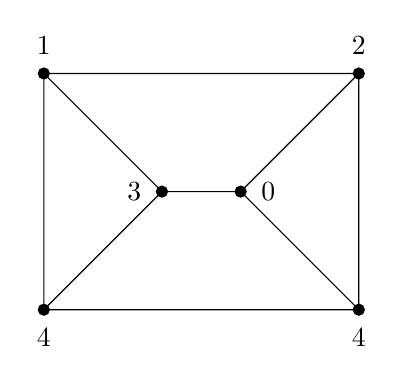
\begin{tikzpicture}
\coordinate (0) at (0.5,0);
\coordinate (3) at (-0.5,0);
\coordinate (1) at (-2,1.5);
\coordinate (2) at (2,1.5);
\coordinate (5) at (-2,-1.5);
\coordinate (4) at (2,-1.5);

\draw (1)--(2)--(4)--(5)--(1)--(3)--(0)--(4);
\draw (5)--(3);
\draw (0)--(2);

\node[xshift=10pt] at (0){0};
\node[yshift=10pt] at (1){1};
\node[yshift=10pt] at (2){2};
\node[xshift=-10pt] at (3){3};
\node[yshift=-10pt] at (4){4};
\node[yshift=-10pt] at (5){4};

\foreach \point in {0,1,2,3,4,5}
\draw[fill=black] (\point) circle (2pt); 
\end{tikzpicture}

\caption{Graf $T(\Z_6)$}
\label{T(Z2xZ3)}
\end{figure}

Totalni graf je v primeru, ko $R$ ni lokalni kolobar, povezan. To nam pove naslednja lema.
\begin{lema}
Naj bo $R$ artinski komutativni enotski kolobar, ki ni lokalen. Potem je $T(R)$ povezan graf.
\end{lema}

\proof
Po izreku 8.7 iz \cite{Atiyah} lahko kolobar $R$ zapišemo kot $R=R_1 \times \dots \times R_n$, kjer so $R_i$ artinski lokalni kolobarji in je $n\ge 2$, ker $R$ ni lokalen. Zadošča pokazati, da obstaja pot med poljubnim vozliščem in 0. Naj bo torej $x=(0,\dots,0)$ in $y\in R$ poljubno drugo vozlišče. Predpostavimo najprej, da je $y$ oblike $y=(y_1,\dots,y_k,0,\dots,0)$, kjer je $1\le k \le n$ in so $y_1,\dots,y_k$ neničelni. Tvorimo zaporedje vozlišč $\{z_i\}_{i=0}^k$, kjer je $z_i = (-1)^i (y_1,\dots, y_{k-i},0\dots,0)$. Pri tem je $z_k = x $ in $z_0 = y$. Pokažimo, da je to pot med $x=0 $ in $y$. Zadošča torej pokazati, da je $z_i $ soseden z $z_{i+1}$. To pa velja, saj je $z_i + z_{i+1} =  (-1)^i (y_1,\dots, y_{k-i},0\dots,0) +  (-1)^{i+1} (y_1,\dots, y_{k-i-1},0\dots,0) = \pm  (0,\dots,0, y_{k-i},0\dots,0)\in Z(R)$. Analogno lahko za $y$ poljubne oblike poiščemo pot med $y$ in $0$. Sledi, da je $T(R)$ povezan.

\endproof

V primeru ko kolobar ni lokalen je lahko določiti premer totalnega grafa. V naslednjem dokazu bomo videli še drugo konstrukcijo neke poti med dvema vozliščema, ki bo obenem še krajša od zgornje.

\begin{lema}
Naj bo $R$ končni komutativni enotski kolobar, ki ni lokalen. Potem je njegov premer $\diam(T(R)) = 2$. 
\end{lema}

\proof
Ker $R$ ni lokalni, je pa končni komutativni enotski kolobar, ga lahko zapišemo kot $R= R_1 \times \dots \times R_n, n\ge 2$, kjer so $R_i$ končni lokalni kolobarji. Naj bosta $x=(x_1,\dots, x_n)$ in $y=(y_1,\dots,y_n)$ poljubni vozlišči grafa $T(R)$. Poiskati moramo pot dolžine dve med njima. Označimo z $z=(-x_1,-y_2,0,\dots,0)$. Potem je $x+z = (0,x_2 - y_2,x_3,\dots,x_n)\in Z(R)$ in $z+y = (y_1 - x_1,0,y_3,\dots,y_n)\in Z(R)$. Iskana pot je torej $x-z-y$.  Jasno je tudi, da med $(0,\dots,0)$ in $(1,\dots,1)$ ni krajše poti.
\endproof

Poglejmo si sedaj, kdaj v totalnem grafu lahko najdemo cikel lihe dolžine.

\begin{lema}
Naj bo $R$ končni komutativni enotski kolobar, ki ni lokalen. Če $R\not\cong \Z_2 \times \Z_2$, potem graf $T(R)$ vsebuje tricikel.
\end{lema}

\proof 
Ker je $R$ končni enotski komutativni kolobar, ga lahko po izreku 8.7 iz \cite{Atiyah} zapišemo kot $R=R_1 \times \dots\times R_n$, kjer so $R_i$ končni lokalni kolobarji. Pri tem je še $n\ge 2$, ker $R$ ni lokalen. Denimo najprej, da je $n\ge 3$. Ker je $R$ enotski, so tudi vsi $R_i$ enotski kolobarji. Označimo z $x_0 = (0,\dots,0), x_1 = (1,0,\dots,0), x_2 = (0,1,0,\dots,0)$. Očitno je $x_0 x_1, x_1 x_2, x_2 x_0 \in E(T(R))$, torej graf $T(R)$ vsebuje tricikel. Naj bo sedaj $n=2$. Velja torej $R= R_1 \times R_2$. Ker je $R\not \cong\Z_2 \times \Z_2$, ima vsaj eden izmed kolobarjev $R_1, R_2$ vsaj tri elemente. Predpostavimo torej lahko, da je $|R_1| \ge 3$. Potem v $R_1 \setminus\{0 \}$ obstajata dva različna elementa $a\neq b$. Označimo spet z $x_0 = (0,0), x_1 = (a,0), x_2 = (b,0)$. Spet velja $x_0 x_1, x_1 x_2, x_2 x_0 \in E(T(R))$, saj je $x_0 + x_1, x_1 + x_2, x_2 + x_0\in Z(R)$. Spet smo našli tricikel v $T(R)$, s čimer smo dokazali lemo.
\endproof

\begin{opomba}
Graf $T(\Z_2 \times \Z_2)$ očitno ne vsebuje tricikla. Glej sliko \ref{T(Z2xZ2)}.
\end{opomba}

\begin{figure}[h!]
\centering
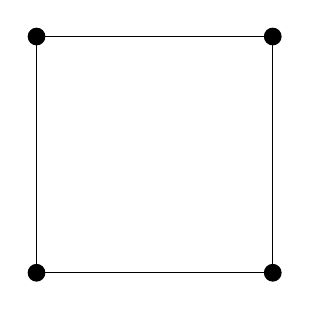
\begin{tikzpicture}
\coordinate (a) at (-1.5,1.5);
\coordinate (b) at (1.5,1.5);
\coordinate (c) at (-1.5,-1.5);
\coordinate (d) at (1.5,-1.5);


\draw (a)--(b)--(d)--(c)--(a);

\foreach \point in {a,b,c,d}
\draw[fill=black] (\point) circle (3pt);

\end{tikzpicture}
\caption{Graf $T(\Z_2 \times \Z_2)$}
\label{T(Z2xZ2)}
\end{figure}

\begin{lema}
Graf je dvodelen natanko tedaj, ko ne vsebuje ciklov lihe dolžine.
\end{lema}

\proof
Glej trditev 1.6.1 v \cite{Diestel}.
\endproof

\begin{posledica}
Kolobar $R=\Z_2 \times \Z_2$ je edini končni enotski komutativni kolobar, ki ni lokalen in ima dvodelen totalni graf $T(R)$.
\end{posledica}

Prav tako znamo sedaj natnačno določiti ožino (velikost najmanjšega cikla v grafu) končnega komutativnega enotskega kolobarja, ki ni lokalen.

\begin{posledica}
Naj bo $R$ končni komutativni enotski kolobar, ki ni lokalen. Potem je njegova ožina enaka 4, če je $R \cong \Z_2 \times \Z_2$ in 3 sicer.
\end{posledica}

Poglejmo si zdaj še totalne grafe lokalnih kolobarjev. Za razliko od prej ti niso povezani.

MOGOČE DODATI PRIMERA TOTALNIH GRAFOV  Z8 in Z9

\begin{izrek}
\label{klasifikacijaT(R)zaLokalenKolobar}
Naj bo $R$ končni lokalni enotski kolobar. Graf $T(R)$ ni povezan. Če je karakteristika $R$ enaka $\textrm{char} (R) = 2^k$, je $T(R)$ izomorfen disjunktni uniji $|R/Z(R)|$ kopij grafa $K_{|Z(R)|}$, sicer pa je $T(R)$ izomorfen disjunktni uniji grafa $K_{|Z(R)|}$ in $\frac{1}{2}(|R/Z(R)| - 1)$ kopij grafa    $K_{|Z(R)|, |Z(R)|}$.
\end{izrek}

\proof
Po lemi \ref{vsotaElementovDeliteljNica} je $x+y \in Z(R)$ natanko tedaj, ko  je $(x+J(R)) + (y+J(R))  \in Z(R/J(R))$. Ker je $R$ lokalni kolobar, je $J(R) = Z(R)$ edini maksimalni ideal. Posledično je $ F = R/Z(R) = R/J(R)$ polje. Ker to nima pravih deliteljev niča, sta dve vozlišči $x$ in $y$ povezani v $T(F)$ natanko tedaj, ko je $x=-y$. 
Če je $\textrm{char}(R) = 2^k$, potem je $\textrm{char}(F) = 2$. To pa pomeni, da je za vsak element $x = -x$, torej je $T(F)$ sestavljen iz $|F| = |R/Z(R)|$ kopij $K_1$. Sledi, da $T(R)$ ni povezan.

Če $\textrm{char}(R) \neq 2^k$, potem $\textrm{char}(F)\neq 2$ in posledično $x\neq -x$ za vsak $x\neq 0$. Sledi, da ima $T(F)$ eno kompononento $K_1$ za vozlišče 0 in $\frac{1}{2}(|F| - 1)$ komponent $K_2$ za ostale pare vozlišč $x$ in $-x$. Spet sledi, da $T(R)$ ni povezan.

 Pokazati moramo še, da $T(R)$ res vsebuje prave komponente.
V prvem primeru, ko je $ \textrm{char}(R) = 2^k$ moramo videti, da so vsi elementi iz odseka povezani med sabo. Vzemimo poljuben odsek $x+Z(R)$. Naj bosta $x+ y_1$ in $x+y_2$ poljubna elementa iz tega odseka. Ker je $x=-x$, je $2x = 0$ in ker je $R$ lokalni kolobar, je $Z(R) = J(R)$ ideal in zato zaprt za seštevanje. Sledi $(x+ y_1 ) + (x+y_2)  = 2x + y_1 +y_2 = y_1 + y_2 \in J(R) = Z(R)$. To implicira, da vsaki kopiji $K_1$ v $T(F)$ pripada kopija $K_{|Z(R)|}$ v $T(R)$. Sledi, da je $T(R)$ v tem primeru res disjunktna unija $|R/Z(R)|$ kopij $K_{|Z(R)|}$.

Poglejmo si zdaj še primer, ko $\textrm{char}(R) \neq 2^k$. Enako kot zgoraj vidimo, da kopiji $K_1$, ki pripada vozlišču $0$ v $T(F)$ v grafu $T(R)$ pripada graf $K_{|Z(R)|}$. Videti moramo le še, da kopiji grafa  $K_2$ ki pripada paru vozlišč $x$ in $-x$ iz grafa $T(F)$ v grafu $T(R)$ pripada graf $K_{|Z(R)|, |Z(R)|}$. Naj bo $x+ y_1\in x  + Z(R)$ in $-x + y_2\in -x + Z(R)$, kjer je $x\neq 0$. Potem je $(x+y_1) + (-x + y_2 ) = y_1 + y_2\in Z(R)$, ker je $Z(R) = J(R)$ zaprt za seštevanje. Če pa sta $x+y_i \in x + Z(R), i=1,2$, potem je $(x+y_1) + (x+y_2) = 2x + (y_1 + y_2) \in 2x + Z(R) \not\subseteq Z(R)$, saj je $x\neq 0$. Na podoben način vidimo, da tudi elementi, ki pripadajo odseku $-x + Z(R)$ v $T(R)$ niso povezani med sabo. Sledi, da vsaki kopiji $K_2$ iz grafa $T(F)$ v grafu $T(R)$ res pripada kopija $K_{|Z(R)|,|Z(R)|}$.
\endproof

S pomočjo zgornjega izreka lahko karakteriziramo ožino totalnega grafa lokalnega kolobarja.

\begin{posledica}
Naj bo $R$ končni lokalni enotski kolobar. Če je $|Z(R)| \ge 3$, je ožina $\textrm{gr}(T(R)) = 3$, sicer pa je ožina $\textrm {gr}(T(R)) = \infty$.
\end{posledica}

\proof
To sledi iz izreka \ref{klasifikacijaT(R)zaLokalenKolobar}. Če je $\textrm{char}(R) = 2^k$, potem graf $T(R)$ vsebuje kopijo grafa $K_{|Z(R)|}$, ki v primeru, ko je $|Z(R)| \ge 3$ vsebuje tricikel. Če pa je $|Z(R)| \in \{1,2\}$, potem je $T(R)$ sestavljen iz samih disjunktnih kopij grafov $K_1$ ali grafov $K_2$, ki pa sploh ne vsebujejo cikla. V tem primeru je $\textrm{gr}(T(R)) = \infty$. Podobno je v primeru, ko $\textrm{char}(R) \neq 2^k$ in $|Z(R)| \ge 3$, spet $\textrm{gr}(T(R)) = 3$, saj $T(R)$ vsebuje kopijo $K_{Z(R)}$. Denimo torej, da $\textrm{char}(R) \neq 2^k$ in je $|Z(R)| \le 2$. Poglejmo si najprej primer, ko je $|Z(R)| = 1$. Tedaj je $T(R)$ disjunktna unija podgrafa $K_1$ in $\frac{1}{2}(|R| - 1)$ kopij grafa $K_{1,1} = K_2$. Nobeden izmed teh grafov ne vsebuje cikla, torej je $\textrm{gr} (T(R)) = \infty$. Naj bo zdaj še $|Z(R)| = 2$. Ker smo v lokalnem primeru, je $Z(R) = J(R)$ in ker je to podgrupa, deli moč kolobarja $R$. Po posledici 2.4 iz \cite{diploma} je moč lokalnega kolobarja praštevilo. Sledi, da je $|R| = 2^n$. Ker pa po \ref{charDeliMocKolobarja} karakteristika deli moč kolobarja, mora biti $\textrm{char}(R) = 2^k$. Protislovje. Sledi, da tak kolobar sploh ne obstaja.
\endproof

Sedaj si bomo pogledali regularnost totalnega grafa. Pri tem nam bodo v pomoč naslednje leme.

\begin{lema}
\label{regular1}
Naj bo $R$ končni komutativni kolobar. Naj bo $x$ poljubno vozlišče grafa $T(R)$. Če velja $x+x = 2x \notin Z(R)$, je stopnja $x$ enaka $\deg(x) = |Z(R)|$, sicer pa je $\deg(x) = |Z(R)| -1$. Velja še, da je  $2\in Z(R)$ natanko tedaj, ko je $T(R)$ $(|Z(R)| - 1)$-regularen graf. 
\end{lema}

\proof
Naj bo $x$ poljubno vozlišče grafa $T(R)$. Za vsak $z\in Z(R)$ lahko definiramo element $a = z -x \in R$. Potem velja $a + x = z\in Z(R)$. To pomeni, da je $x$ povezan z $a$, razen če je $x=a$. Če je torej $x$ tak, da je $x+x = 2x \in Z(R)$, je $\deg(x) = |Z(R)| - 1$, ker $x$ ni povezan sam s sabo. Če pa $x+x=2x \notin Z(R)$, je za vsak $z\in Z(R)$ element $z-x \neq x$. Sledi $\deg(x) = |Z(R)|$.

Dokažimo še drugi del leme. Denimo najprej, da $2\notin Z(R)$. Vemo, da je vozlišče 0 povezano le z neničelnimi elementi iz $Z(R)$, torej $\deg(0)=  |Z(R)| -1 $. Potem je $\deg(1) = |Z(R) | \neq |Z(R)| - 1= \deg(0)$ in posledično graf $T(R)$ ni regularen. 
Dokažimo še obrat. Denimo, da $2  \in Z(R)$. Potem je zaradi komutativnosti za vsak $x\in R$ tudi $2x\in Z(R)$. Po prvem delu leme tako sledi, da je za vsak $x\in R$ stopnja $\deg(x) = |Z(R)| - 1$, kar pa ravno pomeni, da je $T(R)$ res $(|Z(R)| -1)$-regularen graf.
\endproof

\begin{lema}
\label{regular2}
Naj bo $R$ končni komutativni enotski kolobar. Potem je $2\in Z(R)$ natanko tedaj, ko $2$ deli $|R|$.
\end{lema}

\proof
Naj bo najprej $R$ lokalni kolobar. Če $2$ deli $|R|$, je po posledici 2.4 iz \cite{diploma} $|R| = 2^n$. Po \ref{charDeliMocKolobarja} je $\textrm{char}(R) = 2^k, k > 1$, torej je $2 \cdot 2^{k-1} = 0$ in posledično je $2\in Z(R)$. 
Dokažimo še obrat. Naj bo $2\in Z(R)$. Potem obstaja $x\in R\setminus{0}$, da je $2x = 0$. Če je $n = \textrm{char}(R)$, potem mora 2 deliti $n$, sicer $nx\neq 0$. Po lemi \ref{charDeliMocKolobarja} pa $n$ deli $|R|$ in ker je relacija deljivosti tranzitivna, 2 deli $|R|$.

Če pa $R$ ni lokalen, ga lahko zapišemo kot $R = R_1 \times \dots \times R_n$, kjer so $R_i$ lokalni kolobarji. Enoto 1 kolobarja $R$ enačimo z elementom $(1,\dots,1)\in R_1 \times \dots \times R_n$. Potem element $2 = 1+1 = 2 \cdot 1$ enačimo z $2\cdot (1,\dots,1)$. Če $2$ deli $|R|$, mora biti vsaj eden izmed kolobarjev $R_i$ sode moči in ker je lokalen, mora biti moči $2^k$. Predpostavimo lahko, da je to $R_1$. Po prvem delu sledi, da je $2\in Z(R_1)$ in posledično je $2(1,\dots,1) \in Z(R_1\times \dots \times R_n)$. Če pa je $2\in Z(R)$, je $2\cdot (1,\dots,1) \in Z(R_1\times \dots \times R_n)$. Spet sledi, da obstaja indeks $i$, da je $2\in Z(R_i)$. Po prvem delu sledi, da 2 deli $|R_i|$. Ker je $|R| = \prod_{i=1}^n |R_i|$, sledi, da 2 deli $|R|$.
\endproof

\begin{lema}
\label{regular3}
Naj bo $R$ končni komutativni enotski kolobar. Če je $|R|$ liho število, je $|U(R)|$ sodo število.
\end{lema}

\proof
Naj bo najprej $R$ lokalni kolobar. Potem je po posledici 2.4 iz \cite{diploma} $|R| = p^n$, kjer je $p$ praštevilo. Če je $|R|$ liho število, je $p\neq 2$. Ker je $R$ končen, je vsak njegov element bodisi obrnljiv bodisi delitelj niča. Vsi delitelji niča so torej ravno v edinem maksimalnem idealu $J(R)$, ki pa je moči $p^k, k < n$. Ker je $U(R) = R \setminus Z(R) = R \setminus J(R)$, je $|U(R)| = |R| - |J(R) | = p^n - p ^k = p^k(p^{n-k} -1)$. Ker je $n>k$, je $p^{n-k}$ liho število in posledično je $|U(R)|$ sodo število. Če pa $R$ ni lokalen, ga lahko zapišemo kot $R= R_1 \times \dots \times R_n$, kjer so $R_i$ končni lokalni kolobarji. Ker je $|R|$ liho število, je za vsak $i$ tudi $|R_i|$ liho število. Po prvem delu je tako $|U(R_i)| $ sodo število. Ker pa je $U(R) = U(R_1) \times \dots \times U(R_n)$, je $|U(R)| = \prod_{i=1}^n |U(R_i)|$ produkt sodih števil in zato sodo število.
\endproof

Če zadnje tri leme združimo, dobimo naslednji izrek.

\begin{izrek}
\label{regularnostT(R)}
Naj bo $R$ končni komutativni enotski  kolobar. Tedaj velja:
 \begin{enumerate}
\item če je $|R|$ sodo število, je $T(R)$ $(|Z(R)| -1)$-regularen graf,
\item če je $|R|$ liho število, je za $x\in Z(R)$ stopnja $\deg(x) = |Z(R)| - 1$ in za $x\in U(R)$ je stopnja $\deg(x) = |Z(R)|$.
\end{enumerate}
\end{izrek}

\proof
Po lemi \ref{regular1} je $T(R)$ $(|Z(R)| -1)$-regularen graf natanko tedaj, ko je $2\in Z(R)$, kar je po lemi \ref{regular2}  res natanko tedaj, ko je $|R|$ sodo število. Če pa je $|R|$ liho število, potem po lemi \ref{regular2} sledi, da $2\notin Z(R)$. Če je $x \in U(R)$, potem tudi $2x\notin Z(R)$. Po lemi \ref{regular1} je potem $\deg(x) = |Z(R)|$. Naj bo torej $x\in Z(R)$. Obstaja torej $y\in R \setminus \{0\}$, da je $xy=0$. Če je $2x \neq 0$, je $(2x) y = 2(xy) = 0$ in je $2x\in Z(R)$ in je zato po lemi \ref{regular1} $\deg(x) = |Z(R)|-1$. Če pa je $2x = 0$, pa zaključimo, da je $x=0$, saj po predpostavki velja $2\notin Z(R)$. Element $x=0$ je povezan z vsemi delitelji niča razen z 0, torej je tudi v tem primeru $\deg(x) = \deg(0) = |Z(R)| - 1$.
\endproof

% RAVNINSKOST TOTALNEGA GRAFA
\section{Ravninskost totalnega grafa}

Poglejmo si najprej primer, ko je $R$ cel kolobar. Potem je vozlišče $x$ povezano edino z vozliščem $-x$ in še to le v primeru, ko je $x\neq -x$. Sledi, da je graf $T(R)$ disjunktna unija podgrafov $K_1$ in $K_2$. Očitno je torej ravninski. V posebnem to seveda velja za vsa polja. Omejimo se sedaj na končne komutativne enotske kolobarje.  Najprej si bomo pogledali primer, ko imamo lokalni kolobar, potem pa še primer, ko je $R$ splošen končni komutativni enotski kolobar.

% RAVNINSKOST TOTALNEGA GRAFA LOKALNIH KOLOBARJEV
\subsection{Lokalni kolobarji}

Naj bo $R$ končni komutativni lokalni enotski kolobar. Po \cite[Posledica 2.4]{diploma} je $|R| = p^n$, kjer je $p$ praštevilo in $n\ge 1$. Po lemi \ref{charDeliMocKolobarja} in izreku \ref{klasifikacijaT(R)zaLokalenKolobar} je v primeru, ko je $p=2$ graf $T(R)$ izomorfen disjunktni uniji $|R/Z(R)|$ kopij $K_{|Z(R)|}$, sicer pa je $T(R)$ izomorfen disjunktni uniji grafa $K_{|Z(R)|}$ in $\frac{1}{2}(|R/Z(R)| - 1)$ kopij grafa $K_{|Z(R)|,|Z(R)|}$.
Predpostavimo lahko, da $R$ ni polje, saj smo zgoraj videli, da je totalni graf poljubnega polja ravninski. Označimo z $m$ še edini maksimalni ideal kolobarja $R$. Ker je $R$ lokalen, je $m=J(R) = Z(R)$. Ker pa $R$ ni polje in je $|R|=p^n, n \ge 2$, je  $|m| = p^k, 1\le k < n$. Ločimo nekaj primerov glede na to, kakšen je $p$. Če je $R$ kolobar moči $p ^n$, kjer je praštevilo $p\ge5$, potem je $|Z(R)| = |m| \ge 5$. Sledi, da $T(R)$ vsebuje minor $K_5$ in  zato ni ravninski. Ostaneta nam torej možnosti $p=3$ ali $p=2$. Najprej si poglejmo primer, ko je $p=3$. Tedaj je $|R|= 3^n, n\ge  2$ in $|m| = 3^k$, kjer je $1\le k \le n-1$, ker $R$ ni polje in ima enoto. Sledi, da je $|R/Z(R)| \ge 3$ in zato $T(R)$ vsebuje vsaj eno kopijo $K_{|Z(R)|,|Z(R)|}$. Ker je $Z(R)= m$ in je $|m| \ge 3$, graf $T(R)$ vsebuje podgraf $K_{3,3}$, ki ni ravninski. Sledi, da tudi $T(R)$ v tem primeru ni ravninski. Obravnavajmo še primer, ko je $p=2$. Tedaj je $|R| = 2^n, n\ge 2$ in $|m| = 2^k, 1 \le k \le n-1$. Če je $k\ge 3$, potem graf $T(R)$ vsebuje minor $K_5$ in ni ravniski. Če pa je $k=2$, je graf $T(R)$ izomorfen disjunktni uniji $2^{n-2}$ kopij $K_{2^2} = K_4$ (seveda mora biti $n\ge 3$). V tem primeru je $T(R)$ ravninski. Če pa je $k=1$, je $T(R)$ izomorfen disjunktni uniji $2^{n-1}$ kopij grafa $K_2$. Tudi v tem primeru je $T(R)$ ravninski. 

Zgornje ugotovitve lahko strnemo v naslednjo trditev.

\begin{trditev}
Naj bo $R$ končni komutativni lokalni enotski kolobar. Če je $T(R)$ ravninski graf, potem je bodisi $R$ polje bodisi je $|R| = 2^n, n\ge 2$ in $|m| = 2$ ali $|m| = 4$, kjer je $m$ edini maksimalni ideal lokalnega kolobarja $R$.
\end{trditev}

% RAVNINSKOST TOTALNEGA GRAFA NELOKALNIH KOLOBARJEV
\subsection{Nelokalni kolobarji}

Vemo že, da vsak končni komutativni enotski kolobar $R$ lahko zapišemo kot $R= R_1 \times \dots \times R_n$, kjer so $R_i$ lokalni kolobarji. Določimo sedaj minimalne praideale v kolobarju $R$. Če je $R$ tak kot zgoraj, potem vpeljimo še oznako $e_i = (0,\dots,0,1,0,\dots,0)$, kjer je enica na $i$-tem mestu. Element $e_i$ ima torej na vseh komponentah ničle, le na $i$-ti ima enico. Od tod jasno sledi, da za množico $\{e_i\}_{i=1}^n$ velja $e_i \cdot e_j = \delta_{ij}$.

Začnimo s prvo lemo. 
\begin{lema}
\label{minPra1}
Naj bo $R=R_1 \times \dots \times R_n, n\ge 2,$ končni komutativni enotski kolobar in naj bodo $R_i$ končna polja. Potem je množica $\{P_i\}_{i=1}^n$, kjer je $P_i = R_1 \times \dots \times R_{i-1} \times \{0\} \times R_{i+1} \times \dots \times R_n$, ravno množica vseh minimalnih praidealov kolobarja $R$.
\end{lema}

\proof
Za vsak minimalni praideal $P$ obstaja indeks $i$, da $e_i\notin P$, sicer je $P = R$ in sploh ni pravi ideal. Označimo s $Q_i$ množico elementov, za katero želimo, da je minimalni praideal in da ne vsebuje elementa $e_i$. Množica $Q_i$ zagotovo vsebuje $0$. Ker je za vsak $j\neq i$ produkt $e_j e_i = 0\in Q_i$ in ker želimo, da je $Q_i$ praideal za katerega velja $e_i \notin Q_i$, mora $Q_i$ vsebovati vse $e_j, j\neq i$. Če želimo, da je $Q_i$ ideal, mora biti zaprta za seštevanje in zato je $ R_1 \times \dots \times R_{i-1} \times \{0\} \times R_{i+1} \times \dots \times R_n \subseteq Q_i$. Ta množica je očitno ideal. Je tudi praideal, ker je $R_i$ polje. Po konstrukciji je minimalen praideal, ki ne vsebuje $e_i$. Dobili smo ravno $P_i$.

Pokažimo še, da mora vsak praideal vsebovati vse razen enega izmed elementov $e_i$. Denimo nasprotno, da je $P$ neki praideal, ki ne vsebuje elementov $e_i,e_j, i\neq j$. Velja $e_i e_j = 0\in P$, vendar $e_i,e_j \notin P$. Sledi, da $P$ ni praideal. Protislovje. 
Od tod sledi, da nam zgornja konstrukcija res da vse minimalne praideale, torej je množica vseh minimalnih praidealov res enaka $\{P_i\}_{i=1}^n$.
\endproof

Poglejmo si sedaj še, kaj se zgodi, če kateri izmed faktorjev $R_i$ v prejšnji lemi ni polje.

\begin{lema}
\label{minPra2}
Naj bo $R$ končni komutativni enotski kolobar, ki ni lokalen. Zapišemo ga lahko kot $R = R_1 \times \dots \times R_n, n\ge2$, kjer so $R_i$ lokalni kolobarji. Označimo z $m_i$ edini maksimalni ideal kolobarja $R_i$. Potem je množica $\{P_i\}_{i=1}^n$, kjer je $P_i = R_1 \times \dots \times R_{i-1} \times m_i \times R_{i+1} \times \dots \times R_n$, ravno množica vseh minimalnih praidealov kolobarja $R$.
\end{lema}

\proof
Če so vsi faktorji $R_i$ polja, potem trditev sledi po prejšnji lemi \ref{minPra1}. Denimo torej, da so $R_1, \dots,R_k, k\le n,$ lokalni kolobarji, ki niso polja. Enako kot zgoraj vidimo, da so minimalni praideali , ki ne vsebujejo elementov $e_{k+1}, \dots, e_n$ enaki kot zgoraj. To se ujema tudi s trditvijo te leme, saj je $m_i = 0$ za $k+1 \le i \le n$, ker so pripadajoči kolobarji polja. 
Naj bo torej $1 \le i \le k$. Naj bo spet $Q_i$ množica elementov, ki ne vsebuje $e_i$ in za katero želimo, da je minimalni praideal, za katerega to velja. Enako kot zgoraj vidimo, da mora biti $R_1 \times \dots \times R_{i-1} \times \{0\} \times R_{i+1} \times \dots \times R_n \subseteq Q_i$. Ta množica pa ne more biti praideal, saj obstajata $x_i,y_i\in m_i$, da je $x_i y_i = 0$. Potem je $(x_i e_i ) \cdot (y_i e_i) = 0$ in moramo v $Q_i$ dodati vsaj enega izmed elementov $x_i e_i, y_i e_i$. Vprašanje je, koliko elementov moramo še dodati v $Q_i$, da bo to praideal. Lotimo se tega sistematično. Ker je $R_i$ končen, je $m_i$ nilpotenten. Izberimo najmanjši $l\in  \N$, da je $m_i^l = 0$. Potem moramo zagotovo v $Q_i$ dodati množico elementov $m_i^{l-1} e_i$. Ko dodamo te elemente, množica $Q_i$ še vedno ni praideal, saj $m_i^{l-2}$ brez enote in zato obstajata $y_{l-2},z_{l-2}\in m_i^{l-2} \setminus m_i^{l-1}$, da je $y_{l-2}z_{l-2} \in m_i^{l-1}$. Dodati moramo torej tudi vse elemente $m_i^{l-2}e_i$. Z enakim argumentom pridemo do tega, da moramo v $Q_i$ dodati vse elemente oblike $m_i e_i$. Množica $Q_i$ torej vsebuje vse elemente oblike $R_1 \times \dots \times R_{i-1} \times m_i \times R_{i+1} \times \dots \times R_n$. Ta množica je očitno praideal, ker je $m_i$ praideal. Ker je $m_i$ ideal, tudi ne vsebuje elementa $e_i$. Po konstrukciji je minimalni praideal, za katerega to velja. S tem smo dobili ravno $P_i$.
Enako kot zgoraj premislimo še, da so to res vsi minimalni praideali.
\endproof

Sedaj bomo zgoraj ugotovljeno s pridom uporabili. Po trditvi 4.7 iz \cite{Atiyah} lahko množico vseh deliteljev niča zapišemo kot unijo minimalnih  praidealov kolobarja $R$.

\begin{posledica}
\label{deliteljiNicaUnijaMinPra}
Naj bo $R$ končni komutativni enotski kolobar, ki ni lokalen. Zapišemo ga lahko kot $R = R_1 \times \dots \times R_n, n\ge2$, kjer so $R_i$ lokalni kolobarji. Označimo z $m_i$ edini maksimalni ideal kolobarja $R_i$. Potem je $Z(R) = \cup_{i=1}^n P_i$, kjer je $P_i = R_1 \times \dots \times R_{i-1} \times m_i \times R_{i+1} \times \dots \times R_n$.
\end{posledica}

Naj bo zdaj $P_i$ minimalni praideal kolobarja $R$. Potem je $P_i \subseteq Z(R)$. Ker je $P_i + P_i \subseteq P_i \subseteq Z(R)$, vsakemu minimalnemu praidealu v totalnem grafu $T(R)$ pripada polni podgraf $K_{|P_i|}$. Pri tem velja še, da je $|P_i| = |R_1|\cdots |R_{i-1}| \cdot |m_i| \cdot |R_{i+1}| \cdots |R_n|$.
S pomočjo tega kriterija bomo obravnavali ravninskost totalnega grafa, pomagali pa si bomo še z naslednjim izrekom.

\begin{izrek}(Wagner)
Graf je ravninski natanko tedaj, ko nima minorja izomorfnega $K_5$ ali $K_{3,3}$.
\end{izrek}
Dokaz tega izreka se nahaja v \cite[Theorem 4.2.9]{Diestel}. Pri tem pripomnimo še, da v primeru, ko graf vsebuje podgraf izomorfen $K_l$, kjer je $l\ge5$, vsebuje tudi minor $K_5$.

Ločimo nekaj primerov:
\begin{enumerate}
\item $n\ge 4$. Ker je $|R_i| \ge 2$, je za minimalni praideal $P_1$ zagotovo res $|P_1| = |m_1| \cdot \prod_{i=2}^n |R_i| \ge \prod_{i=2}^n 2 = 2^{n-1}\ge 2^3 = 8$ in zato $T(R)$ v tem primeru vsebuje minor $K_5$ in posledično ni ravninski.

\item $n=3$. V tem primeru je torej $R$ oblike $R= R_1 \times R_2 \times R_3$, kjer je $R_i$ lokalni kolobar moči $p_i^{k_i}$. Predpostavimo lahko, da je $2\le p_1 \le p_2 \le p_3$. Poglejmo si najprej primer, ko sta $p_2, p_3 > 2$. Potem moč minimalnega praideala $P_1 = m_1\times  R_2 \times R_3$ lahko ocenimo kot $|P_1| = |m_1| |R_2| |R_3| >4$, torej $T(R)$ v tem primeru zagotovo vsebuje minor $K_5$ in zato ni ravninski. Oglejmo si sedaj možnost, ko je $p_2 = 2$. Ker je $p_1\le p_2$, je tudi $p_1=2$. Če je pri tem še $p_3 \ge 3$, potem spet lahko ocenimo moč minimalnega praideala $P_1$ kot $|P_1| = |m_1||R_2||R_3| \ge 2\cdot 3 = 6$ in zato spet vsebuje minor $K_5$ in posledično ni ravninski. Ostane nam torej še primer, ko je $p_1 = p_2 = p_3 = 2$. Spet lahko predpostavimo, da je $1\le k_1 \le k_2 \le k_3$. Če je $k_3 \ge 2$, je možno moč minimalnega praideala oceniti kot $|P_1| = |m_1| |R_2||R_3| \ge 2 \cdot 2^2 = 8$ in zato $T(R)$ spet vsebuje minor $K_5$. Posledično tudi v tem primeru ni ravninski. Če pa je $k_3=1$, zaradi predpostavke $1 \le k_1 \le k_2 \le k_3$ sledi $k_1 = k_2 = k_3 = 1$. Kolobar $R$ je v tem primeru enak $R= \Z_2 \times \Z_2 \times \Z_2$. Njegov graf je na sliki \ref{T(Z2xZ2xZ2)}. Če v njem skrčimo povezave $(1,1,0)-(0,0,0),(1,0,0)-(0,0,0),(1,0,1)-(0,0,0)$, dobimo minor $K_5$ in zato $T(Z_2 \times Z_2 \times Z_2)$ ravno tako ni ravninski graf.

\begin{figure}[h!]
\centering
% T(Z_2 x Z_2 x Z_2)
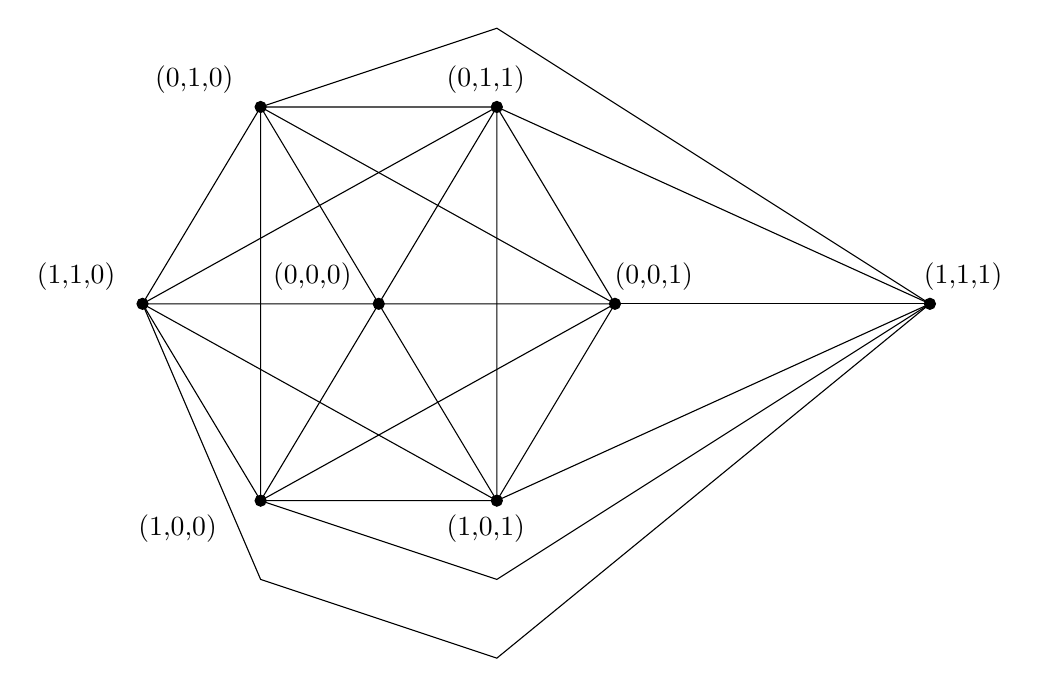
\begin{tikzpicture}
\coordinate (000) at (-1,0);
\coordinate (001) at (2,0);
\coordinate (011) at (0.5,2.5);
\coordinate (010) at (-2.5,2.5);
\coordinate (110) at (-4,0);
\coordinate (100) at (-2.5,-2.5);
\coordinate (101) at (0.5,-2.5);
\coordinate (111) at (6,0);

% pomozna vozlisca
\coordinate (zg) at (0.5,3.5);
\coordinate (sp1) at (0.5,-3.5);
\coordinate (sp2) at (0.5,-4.5);
\coordinate (sp3) at (-2.5,-3.5);

\draw (110)--(000)--(001)--(011)--(010)--(110)--(100)--(101)--(001);
\draw (010)--(000)--(101);
\draw (100)--(000)--(011);
\draw (110)--(011)--(101)--(110);
\draw (010)--(001)--(100)--(010);
\draw (111)--(011);
\draw (111)--(001);
\draw (111)--(101);
\draw (111)--(zg)--(010);
\draw (111)--(sp1)--(100);
\draw (111)--(sp2)--(sp3)--(110);

\node[xshift=-24pt,yshift=10pt] at (000){(0,0,0)};
\node[xshift=14pt,yshift=10pt] at (001){(0,0,1)};
\node[yshift=10pt,xshift=-24pt] at (010){(0,1,0)};
\node[yshift=10pt,xshift=-4pt] at (011){(0,1,1)};
\node[xshift=-30pt,yshift=-10pt] at (100){(1,0,0)};
\node[xshift=-4pt,yshift=-10pt] at (101){(1,0,1)};
\node[xshift=-24pt,yshift=10pt] at (110){(1,1,0)};
\node[xshift=12pt,yshift=10pt] at (111){(1,1,1)};


\foreach \point in {000,001,010,011,100,101,110,111}
\draw[fill=black] (\point) circle (2pt); 
\end{tikzpicture}

\caption{Graf $T(\Z_2\times \Z_2 \times  \Z_2)$}
\label{T(Z2xZ2xZ2)}
\end{figure}

\item $n=2$. V tem primeru kolobar $R$ lahko zapišemo kot $R= R_1 \times R_2$, kjer sta $R_1$ in $R_2$ lokalna kolobarja. Njuni moči sta enaki $|R_1 | = p_1^{k_1}$ in $|R_2| = p_2^{k_2}$, kjer sta $p_1$ in $p_2$ praštevili in $k_1,k_2 \ge 1$. Pri tem lahko predpostavimo, da je $2 \le p_1 \le p_2$. Če je $p_2 \ge 5$, lahko moč minimalnega praideala $P_1$ navzdol ocenimo z $|P_1| = |m_1| |R_2| \ge 5$. To pomeni, da $T(R)$ v tem primeru vsebuje minor $K_5$ in zato ni ravninski. Poglejmo si sedaj primer, ko je $p_2 <5$. Potem je bodisi $p_2=2$ bodisi je $p_2 = 3$. Začnimo s primerom $p_2=3$. Potem je po predpostavki $2 \le p_1 \le 3 = p_2$. Če je $p_1=3$, lahko predpostavimo, da je $1\le k_1 \le k_2$. Če je $k_2\ge 2$, potem lahko ocenimo moč minimalnega praideala $P_1$ kot $|P_1| = |m_1||R_2| \ge 3^2 = 9$. Graf $T(R)$ torej vsebuje minor $K_5$ in zato ni ravninski. Če pa je $k_2=1$, je tudi $k_1=1$ in imamo kolobar $R= \Z_3 \times \Z_3$. Njegov graf je na sliki \ref{T(Z3xZ3)}. Če v njem skrčimo povezave $(0,2)-(0,0), (0,1)-(0,0), (1,0)-(0,0), (2,0)-(0,0)$ in odstranimo zanke in večkratne povezave, dobimo ravno graf $K_5$. Sledi, da $T(R)$ v tem primeru ni ravninski.

\begin{figure}[h!]
\centering
% T(Z_3 x Z_3)
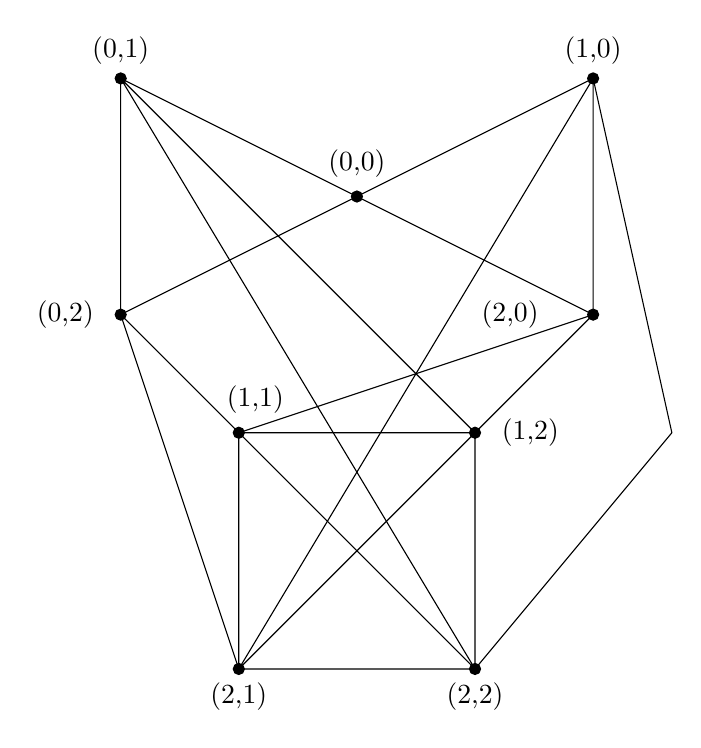
\begin{tikzpicture}
\coordinate (00) at (0,0);
\coordinate (01) at (-3,1.5);
\coordinate (02) at (-3,-1.5);
\coordinate (10) at (3,1.5);
\coordinate (20) at (3,-1.5);
\coordinate (11) at (-1.5,-3);
\coordinate (12) at (1.5,-3);
\coordinate (21) at (-1.5,-6);
\coordinate (22) at (1.5,-6);

% pomozna vozlisca
\coordinate (pom) at (4,-3);

\draw (00)--(10)--(20)--(00)--(01)--(02)--(00);
\draw (11)--(12)--(22)--(21)--(11)--(22);
\draw (21)--(12);
\draw (11)--(02)--(21);
\draw (11)--(20)--(12);
\draw (22)--(01)--(12);
\draw (21)--(10)--(pom)--(22);

\node[yshift=12pt] at (00){(0,0)};
\node[yshift=10pt] at (01){(0,1)};
\node[xshift=-20pt] at (02){(0,2)};
\node[yshift=10pt] at (10){(1,0)};
\node[xshift=-30pt] at (20){(2,0)};
\node[xshift=6pt,yshift=12pt] at (11){(1,1)};
\node[xshift=20pt] at (12){(1,2)};
\node[yshift=-10pt] at (21){(2,1)};
\node[yshift=-10pt] at (22){(2,2)};


\foreach \point in {00,01,02,10,20,11,12,21,22}
\draw[fill=black] (\point) circle (2pt); 
\end{tikzpicture}

\caption{Graf $T(\Z_3\times \Z_3)$}
\label{T(Z3xZ3)}
\end{figure}

Naj bo zdaj $p_2 = 3$ in $p_1 = 2$. Če je $k_2 \ge 2$, lahko ocenimo moč minimalnega praideala $P_1$ kot $|P_1| = |m_1||R_2| \ge 3^2 = 9$. Graf v tem primeru vsebuje minor $K_5$ in zato ni ravninski. Predpostavimo torej, da je $k_2 = 1$. Če je $k_1 \ge 3$, potem je $|P_2| = |R_1||m_2| \ge 2^3 = 8$ in graf $T(R)$ spet ni ravninski, ker v njem lahko najdemo minor $K_5$. Ostal nam je torej še primer, ko je $k_1= 1$ ali $k_1=2$. Če je $k_1= 1$, je $R= \Z_2 \times \Z_3$. Graf $T(\Z_2 \times \Z_3)$ je ravninski. Glej sliko \ref{T(Z2xZ3)}. Če pa je $k_1 = 2$, pa je $R = R_1 \times Z_3$, kjer je $R_1$ lokalni komutativni enotski kolobar moči 4. Po \cite{Dresden-smallRings} obstajajo štirje komutativni enotski kolobarji moči 4. Ti so $\Z_4, \Z_2 \times \Z_2, \Z_2[x]/(x^2 + 1) = \big\{
\begin{bmatrix}
0 & 0 \\
0 & 0 \\
\end{bmatrix},
\begin{bmatrix}
1 & 0 \\
0 & 1 \\
\end{bmatrix},
\begin{bmatrix}
0 & 1 \\
1 & 0 \\
\end{bmatrix},
\begin{bmatrix}
1 & 1 \\
1 & 1 \\
\end{bmatrix} \big\}, 
\Z_2[x]/(x^2  + x +1) = \big\{
\begin{bmatrix}
0 & 0 \\
0 & 0 \\
\end{bmatrix},
\begin{bmatrix}
1 & 0 \\
0 & 1 \\
\end{bmatrix},
\begin{bmatrix}
1 & 1 \\
1 & 0 \\
\end{bmatrix},
\begin{bmatrix}
0 & 1 \\
1 & 1 \\
\end{bmatrix} \big\}
$. 
Pri tem kolobar $\Z_2 \times \Z_2$ ne pride v poštev, saj je razcepen in zato ni lokalen. Omeniti velja še, da je zadnji kolobar polje. Preverimo še, da je kolobar $\Z_2[x]/(x^2 + 1)$ lokalen. Njegovi elementi so $0,1,x,1+x$. Pri tem sta $1$ in $x$ obrnljiva, $1+x$ pa je delitelj niča. Množica $\{0,1+x\}$ je torej res edini ideal tega kolobarja, ki je zato lokalen. Poglejmo si najprej primer kolobarja $R=\Z_4 \times \Z_3$. Enostavno je videti, da ima množica $Z(R)$  osem elementov, zato je graf $T(R)$ 7-regularen graf. Ker ima precej povezav, tu ne bomo risali njegovega grafa. Opazimo pa, da je $P_1 = m_1 \times R_2 = 	\{0,2\} \times \Z_3$ in zato $|P_1| = 6$. Sledi, da ima $T(R)$ minor $K_6$ in zato tudi $K_5$. Sledi, da $T(R)$ v tem primeru ni ravninski. Podobno velja za $R = \Z_2[x]/(x^2 +1) \times \Z_3$. Tudi tu je minimalni praideal $P_1 = m_1 \times R_2 = \{0,1+x\} \times \Z_3$ in zato je $|P_1| = 6$. Sledi, da tudi v tem primeru graf $T(R)$ ni ravninski, saj vsebuje minor $K_6$. Ostane nam torej le še tretji primer, ko je $R = \Z_2[x]/(x^2 + x + 1) \times \Z_3$. Pri tem je kolobar $\Z_2[x]/(x^2 + x+1)$ polje. Množica obrnljivih elementov $U(R) = \{(1,1),(1,2),(x,1),(x,2),(1+x,1),(1+x,2)\}$. Pri tem sta dva različna elementa iz $U(R)$ v $T(R)$ povezana natanko takrat, ko imata različni drugi komponenti ali pa enako prvo komponento. Sledi, da vozlišča $U(R)$ tvorijo podgraf $K_{3,3}$ grafa $T(R)$. Posledično ta ni ravninski.

Obravnavajmo sedaj še primer, ko  je $p_2 = 2$. Ker je $2 \le p_1 \le p_2 = 2$, je tudi $p_1=2$. Predpostavimo lahko, da je $1 \le k_1 \le k_2$. Če je $k_2 \ge 3$, je moč $|P_1|=|m_1||R_2| \ge 2^3 = 8$. Posledično v tem primeru graf $T(R)$ ni ravninski, saj vsebuje minor $K_5$. Obravnavati moramo še možnosti, ko je $k_2 =2$ ali $k_2 = 1$. Začnimo z drugo, ker je enostavnejša. Če je $k_2=1$, mora biti zaradi naše predpostavke tudi $k_1=1$. Tedaj je $R=\Z_2 \times \Z_2$. Njegov totalni graf je ravninski in je na sliki \ref{T(Z2xZ2)}. 
Naj bo zdaj $k_2 = 2$. Tedaj je bodisi $k_1=1$ bodisi je $k_1 = 2$. Začnimo s prvim primerom. Kolobar $R$ je torej oblike $R=\Z_2 \times R_2$, kjer je $R_2$ komutativni lokalni enotski kolobar moči 4. Zgoraj smo že ugotovili, da obstajajo natanko trije taki kolobarji. Naj bo najprej $R=\Z_2 \times \Z_4$. Njegov graf je na sliki \ref{T(Z2xZ4)}. Če skrčimo povezave $(1,2)-(0,0), (1,0)-(0,2), (1,1)-(0,3)$ in  odstranimo zanke in večkratne povezave, dobimo ravno graf $K_5$. Sledi, da $T(\Z_2 \times \Z_4)$ ni ravninski, ker vsebuje minor $K_5$. 

\begin{figure}[h!]
\centering
% T(Z_2 x Z_4)
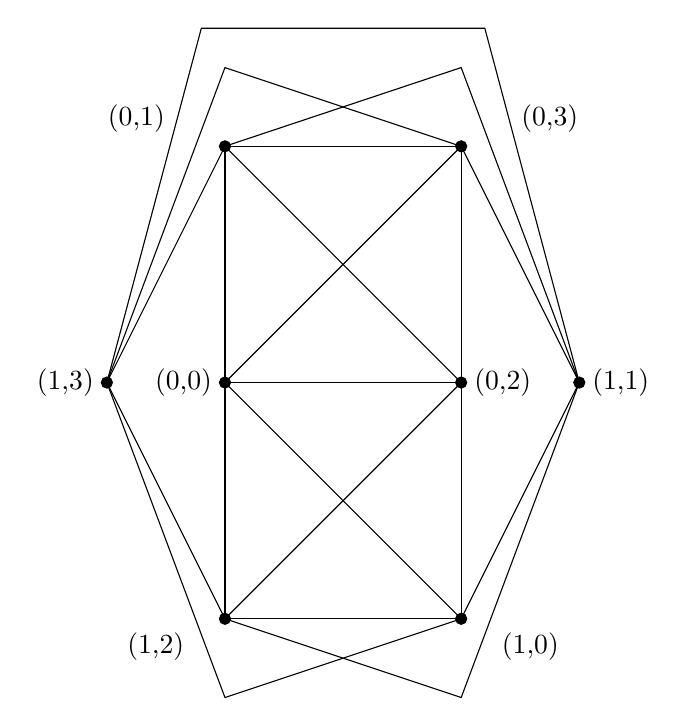
\begin{tikzpicture}
\coordinate (00) at (-1.5,0);
\coordinate (01) at (-1.5,3);
\coordinate (02) at (1.5,0);
\coordinate (03) at (1.5,3);
\coordinate (10) at (1.5,-3);
\coordinate (11) at (3,0);
\coordinate (12) at (-1.5,-3);
\coordinate (13) at (-3,0);

% pomozna vozlisca
\coordinate (spl) at (-1.5,-4);
\coordinate (spd) at (1.5,-4);
\coordinate (zgl1) at (-1.5,4);
\coordinate (zgd1) at (1.5,4);
\coordinate (zgl2) at (-1.8,4.5);
\coordinate (zgd2) at (1.8,4.5);

\draw (00)--(02)--(03)--(01)--(00)--(12)--(10)--(02);
\draw (00)--(03);
\draw (02)--(01);
\draw (12)--(02);
\draw (10)--(00);
\draw (11)--(10)--(spl)--(13)--(zgl1)--(03)--(11);
\draw (13)--(12)--(spd)--(11)--(zgd1)--(01)--(13);
\draw (13)--(zgl2)--(zgd2)--(11);


\node[xshift=-15pt] at (00){(0,0)};
\node[xshift=-32pt,yshift=10pt] at (01){(0,1)};
\node[xshift=15pt] at (02){(0,2)};
\node[xshift=32pt,yshift=10pt] at (03){(0,3)};
\node[xshift=25pt,yshift=-10pt] at (10){(1,0)};
\node[xshift=15pt] at (11){(1,1)};
\node[xshift=-25pt,yshift=-10pt] at (12){(1,2)};
\node[xshift=-15pt] at (13){(1,3)};

\foreach \point in {00,01,02,03,10,11,12,13}
\draw[fill=black] (\point) circle (2pt); 
\end{tikzpicture}

\caption{Graf $T(\Z_2\times \Z_4)$}
\label{T(Z2xZ4)}
\end{figure}

Naslednji je kolobar $R=\Z_2 \times \Z_2[x]/(x^2 + 1)$. Izkaže se, da je njegov totalni graf kar izomorfen totalnemu grafu kolobarja $\Z_2 \times \Z_4$. Preslikava $\varphi : T(\Z_2 \times \Z_2[x]/(x^2 + 1)) \rightarrow T(\Z_2 \times \Z_4)$, ki slika vozlišča takole $\varphi((0,0))=(0,0),\varphi((0,1+x))=(0,2),\varphi((0,1))=(0,1),\varphi((0,x))=(0,3),\varphi((1,1+x))=(1,2),\varphi((1,0))=(1,0),\varphi((1,x))=(1,3),\varphi((1,1))=(1,1)$, je bijekcija med tema dvema grafoma. Sledi, da tudi $T(\Z_2 \times \Z_2[x]/(x^2 + 1))$ ni ravninski. Poglejmo si še primer kolobarja $R=\Z_2 \times \Z_2[x]/(x^2 + x+1)$. Minimalna praideala sta $P_1 = \{0\} \times \Z_2[x]/(x^2 + x+1)$ in $P_2 = \Z_2 \times \{0\}$. Obrnljivi elementi so $U(R) = \{(1,1), (1,x),(1,1+x)\}$. Graf $T(Z(R))$ je ravno $K_4$, ki ima še eno povezavo iz vozlišča $(0,0)$. Graf $T(R)$ pa vsebuje te graf kot podgraf, poleg tega pa kot podgraf vsebuje še tricikel, ki ga sestavljajo vozlišča iz $U(R)$. Poleg tega je v $T(R)$ vozlišče $(1,0)$ povezano še z vsemi vozlišči iz $U(R)$, vsako vozlišče iz $P_1\setminus \{0,0\}$ pa je povezana še s tistim vozliščem iz $U(R)$, ki ima enako drugo komponento. S skrčitvijo povezav med vozliščem $(1,0)$ in vozlišči iz $U(R)$ spet dobimo minor $K_5$. Graf $T(R)$ tudi tokrat ni ravninski. 

Ostal nam je torej le še zadnji primer, ko je $p_1 = p_2 = 2$ in $k_1 = k_2 = 2$. Kolobar $R$ lahko tokrat zapišemo kot $R=R_1 \times R_2$, kjer sta oba kolobarja $R_1$ in $R_2$ komutativna lokalna enotska kolobarja moči 4, torej izomorfna enemu izmed treh zgoraj omenjenih kolobarjev. Obravnavati moramo primere, ko je $R$ izomorfen enemu izmed kolobarjev
\begin{itemize}
\item $\Z_4 \times \Z_4$,
\item $\Z_4 \times \Z_2[x]/(x^2 + 1)$,
\item $\Z_4 \times \Z_2[x] / (x^2 + x+ 1)$,
\item $\Z_2[x]/(x^2+1) \times \Z_2[x]/(x^2+1)$,
\item $\Z_2[x]/(x^2+1) \times \Z_2[x]/(x^2 + x+ 1)$,
\item $\Z_2[x]/(x^2 + x + 1) \times \Z_2[x] / (x^2+x+1)$.
\end{itemize}

V prvih petih primerih si pogledamo minimalni praideal $P_1$. Zaporedoma dobimo $\{0,2\} \times \Z_4, \{0,2\}\times \Z_2[x]/(x^2 + 1), \{0,2\} \times \Z_2[x]/(x^2 + x+1), \{0,1+x\} \times \Z_2[x]/(x^2 + 1), \{0,1+x\} \times \Z_2[x]/(x^2 + x+1)$. Opazimo, da je v vseh petih primerih $|P_1| = 2\cdot 4 = 8$. To implicira, da je $K_8$ podgraf $T(R)$ in zato ta ni ravninski. 
Opazujmo zdaj še zadnji primer, ko je  $R = \Z_2[x]/(x^2 + x + 1) \times \Z_2[x] / (x^2+x+1)$. Trdimo, da tudi tokrat $T(R)$ ni ravninski. V ta namen zadošča pokazati, da podgraf $T(U(R))$ ni ravninski. Ta je na sliki \ref{T(U(R))}. Če skrčimo povezave $(1+x,1+x)-(1+x,x), (1+x,1)-(1+x,x), (x,1+x)-(x,x), (x,1)-(x,x)$, odstranimo zanke in večkratne povezave, dobimo minor $K_5$. Sledi, da $T(U(R))$ ni ravninski in posledično tudi $T(R)$ ni ravninski. 

\begin{figure}[h!]
\centering
% T(U(R))
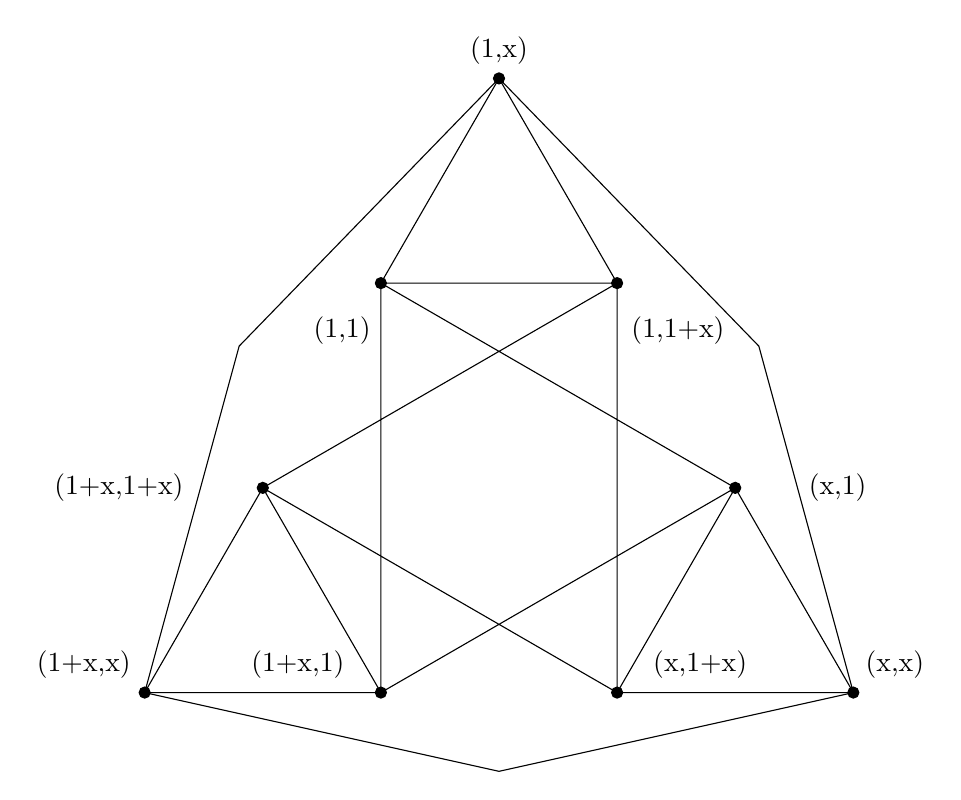
\begin{tikzpicture}
\coordinate (1+xx) at (-4.5,0);
\coordinate (1+x1) at (-1.5,0);
\coordinate (x1+x) at (1.5,0);
\coordinate (xx) at (4.5,0);
\coordinate (1+x1+x) at (-3,2.6);
\coordinate (x1) at (3,2.6);
\coordinate (11) at (-1.5,5.2);
\coordinate (11+x) at (1.5,5.2);
\coordinate (1x) at (0,7.8);

% pomozna vozlisca
\coordinate (s) at (0,-1);
\coordinate (l) at (-3.3,4.4);
\coordinate (d) at (3.3,4.4);

\draw (1+xx)--(1+x1+x)--(11+x)--(1x)--(11)--(x1)--(xx)--(x1+x)--(1+x1+x)--(1+x1)--(11)--(11+x)--(x1+x)--(x1)--(1+x1)--(1+xx);
\draw (1+xx)--(l)--(1x)--(d)--(xx)--(s)--(1+xx);

\node[xshift=-22pt,yshift=10pt] at (1+xx){(1+x,x)};
\node[xshift=-30pt,yshift=10pt] at (1+x1){(1+x,1)};
\node[xshift=30pt,yshift=10pt] at (x1+x){(x,1+x)};
\node[xshift=15pt,yshift=10pt] at (xx){(x,x)};
\node[xshift=-52pt] at (1+x1+x){(1+x,1+x)};
\node[xshift=37pt] at (x1){(x,1)};
\node[xshift=-14pt,yshift=-17pt] at (11){(1,1)};
\node[xshift=22pt,yshift=-17pt] at (11+x){(1,1+x)};
\node[yshift=10pt] at (1x){(1,x)};

\foreach \point in {1+xx,1+x1,x1+x,xx,1+x1+x,x1,11,11+x,1x}
\draw[fill=black] (\point) circle (2pt); 
\end{tikzpicture}

\caption{Graf $T\big(U\big(\Z_2[x]/(x^2 + x + 1) \times \Z_2[x] / (x^2+x+1)\big)\big)$}
\label{T(U(R))}
\end{figure} 

\end{enumerate}

Zgornje ugotovitve lahko združimo v naslednjo trditev.

\begin{trditev}
Edina končna komutativna enotska kolobarja, ki nista lokalna in imata ravninski totalni graf, sta $\Z_2 \times \Z_2$ in $\Z_2 \times \Z_3$.
\end{trditev}

% BARVANJA POVEZAV
\section{O barvanju povezav totalnega grafa}
Poglejmo si sedaj še, kaj lahko povemo o barvanju povezev totalnega grafa. S $\chi'(G)$ bomo označevali \emph{kromatični indeks} grafa $G$, pri čemer je to moč najmanjše množice barv, s katerimi lahko graf pravilno pobarvamo. Jasno je, da kromatični indeks ne more biti strogo manjši kot je maksimalna stopnja grafa. Velja pa še več.

\begin{izrek}(Vizing)
\label{Vizing}
Naj bo $G$ enostaven graf in naj $\Delta$ označuje maksimalno stopnjo grafa $G$. Tedaj je bodisi $\chi'(G) = \Delta$ bodisi $\chi'(G) = \Delta + 1$.
\end{izrek}
Dokaz tega izreka najdemo v \cite[Theorem 5.3.2]{Diestel}.

Za posebne družine grafov je znano, kakšen je njihov kromatični indeks. Takšni so na primer polni grafi in dvodelni grafi. Iz \cite{diploma} se spomnimo, da veljata naslednji lemi.
\begin{lema}
\label{grafKn}
Za $n\ge 2$ je $\chi'(K_n) = n$, če je $n$ liho število in $\chi'(K_n) = n-1$, če je $n$ sodo število.
\end{lema}

\begin{lema}
\label{dvodelenGraf}
Za dvodelen graf $G$ je $\chi'(G) = \Delta(G)$.
\end{lema}
Obravnavo bomo spet razdelili na lokalne in nelokalne kolobarje.

% LOKALNI KOLOBARJI
\subsection{Lokalni kolobarji}
Poglejmo si najprej primer, ko imamo končni komutativni lokalni enotski kolobar.  Tu bo problem lažji, saj že vemo, kakšen je v tem primeru totalni graf. Vemo, da je $|R| = p^n$, kjer je $p$ praštevilo in $n\ge 1$. Po izreku \ref{klasifikacijaT(R)zaLokalenKolobar} vemo, da bo v primeru, ko bo $p=2$ graf $T(R)$ disjunktna unija $|R/Z(R)|$ kopij grafa grafa $K_{|Z(R)|}$, sicer pa bo $T(R)$ disjunktna unija grafa $K_{|Z(R)|}$ in $\frac{1}{2}(|R/Z/(R)| - 1)$ kopij grafa $K_{|Z(R)|,|Z(R)|}$. Ker je v komutativnem lokalnem enotskem kolobarju $Z(R) = m$, kjer je $m$ edini maksimalni ideal, je $|Z(R)| = p^k$, kjer je $0 \le k < n$. V primeru, ko je $p=2$, je po lemi \ref{grafKn} kromatični indeks vsake kopije $K_{|Z(R)|} = K_{2^k}$ enak $2^k -1$. Ker so kopije tega grafa disjunktne med sabo, je tudi $\chi'(T(R)) = 2^k - 1$. Če pa je $p\ge 3$, je $|Z(R)|$ liho število. Po lemi \ref{grafKn} je tedaj kromatični indeks podgrafa $K_{|Z(R)|} = K_{p^k} = p^k$. Ker pa je tudi maksimalna stopnja podgrafa $K_{|Z(R)|,|Z(R)|} = K_{p^k,p^k}$ enaka $p^k$, je po lemi \ref{dvodelenGraf} kromatični indeks podgrafa $K_{|Z(R)|,|Z(R)|} = K_{p^k,p^k}$ tudi enak $p^k$. Ker je v tem primeru graf $T(R)$ sestavljen iz disjunktnih kopij takih grafov, je tudi njegov kromatični indeks $\chi'(T(R)) = p^k$. Te ugotovitve lahko združimo v naslednjo trditev.

\begin{trditev}
\label{kromaticniIndeksT(R)zaLokalniKolobar}
Naj bo $R$ končni komutativni lokalni enotski kolobar. Potem je $|R|=p^n$ in $|Z(R)| = p^k$, kjer je $p$ praštevilo in $n\ge 1, 0 \le k < n$  naravni števili. Kromatični indeks totalnega grafa $\chi'(T(R))$ je enak $2^k -1$, če je $p=2$ in $p^k$ sicer.
\end{trditev}

% NELOKALNI KOLOBARJI
\subsection{Nelokalni kolobarji}
Problem postane težji, če izpustimo predpostavko o lokalnosti, saj v tem primeru totalnega grafa ni moč opisati na tako lep način kot v primeru lokalnega kolobarja. Če združimo izreka \ref{Vizing} in \ref{regularnostT(R)} pa dobimo naslednjo trditev.

\begin{trditev}
Naj bo $R$ končni komutativni enotski kolobar.  Če je $|R|$ sodo število, je $\chi'(T(R)) \in\{|Z(R)|-1, |Z(R)|\}$, sicer pa je $\chi'(T(R)) \in \{|Z(R)|, |Z(R)| +1\}$.
\end{trditev}

\proof
Po izreku \ref{regularnostT(R)} je v primeru, ko je $|R|$ sodo število, graf $T(R)$ $(|Z(R)| - 1)$-regularen graf. To pomeni, da je maksimalna stopnja $\Delta(T(R)) = |Z(R)|-1$ in po Vizingovem izreku \ref{Vizing} trditev v tem primeru sledi. Če pa $|R|$ ni sodo število, pa je za $x\in U(R)$ stopnja $\deg(x) = |Z(R)|$ in za $y \in Z(R)$ je stopnja $\deg(y) = |Z(R)| - 1$. V tem primeru je torej maksimalna stopnja enaka $|Z(R)|$ in z uporabo Vizingovega izreka \ref{Vizing} dobimo trditev.
\endproof

Pripomnil bi še, da ta trditev seveda velja tudi v primeru, ko je $R$ lokalni kolobar. Spomnimo se, da je za lokalni kolobar $R$ sode moči veljalo $\chi'(T(R)) = |Z(R)| -1$, če pa je bil $R$ lokalni kolobar lihe moči, pa je veljalo $\chi'(T(R)) = |Z(R)|$.

Poglejmo si sedaj družino kolobarjev oblike $R(p,k) = \Z_2 \times \GF(p^k)$, kjer je $p$ praštevilo in $k\ge1$ naravno število. Totalni graf takega kolobarja znamo natančneje opisati, kar nam bo tudi v pomoč pri določitvi njegovega kromatičnega indeksa. Najprej ugotovimo, da sta minimalna praideala enaka $P_1= \{0\} \times \GF(p^k)$ in $P_2 = \Z_2 \times \{0\} = \{(0,0),(1,0)\}$. Ker je $Z(R) = P_1 \cup P_2$, je $|Z(R)| = p^k + 1$. Množica obrnljivih elementov pa je enaka $U(R(p,k)) = \{1\} \times \GF(p^k)^*$ in zato moči $|U(R(p,k))| = |\GF(p^k)| = p^k - 1$. Ker je $1+1=0$ v $\Z_2$, sta poljubni vozlišči iz množice $U(R(p,k))$ povezani med sabo v $T(R(p,k))$, saj ima njuna vsota na prvi komponenti 0. Vozlišča iz $U(R(p,k))$ torej napenjajo polni podgraf $K_{p^k -1}$. Od prej pa že vemo, da tudi elementi vsakega minimalnega praideala napenjajo podgraf. Praideal $P_1$ napenja podgraf $K_{p^k}$ in praideal $P_2$ napenja podgraf $K_2$, pri čemer imata ta dva podgrafa skupno vozlišče $(0,0)$. Poleg tega imamo v grafu $T(R(p,k))$ še povezavo med vozliščem $(1,0)\in P_2$ in poljubnim vozliščem iz $U(R(p,k))$, ter za vsak neničelni $x\in \GF(p^k)$ še  povezavo med vozliščem $(0,x)\in P_1$ in vozliščem $(1,-x)\in U(R(p,k))$. Zapišimo to formalno. Ker je $|R(p,k))| = 2p^k$, ima graf $T(R(p,k))$ $2p^k$ vozlišč. Označimo jih kot $V(T(R(,p,k))) = \{v_i\}_{i=1}^{p^k} \cup \{u_i\}_{i=1}^{p^k}$. Pri tem vozlišče $u_1$ enačimo z vozliščem $(0,0)$, vozlišče $v_1$ pa z vozliščem $(1,0)$. Množica povezav je tedaj enaka $E(T(R(p,k))) = \{u_i u_j\}_{1\le i < j \le p^k} \cup \{v_i v_j\}_{1\le i < j \le p^k} \cup \{u_i v_i\}_{i=1}^{p^k}$. S tem je graf $T(R(p,k))$ natančno določen.

Poglejmo si sedaj, kaj lahko povemo o kromatičnem indeksu $\chi'(T(R(p,k)))$.  Pri tem bomo spet ločili dva primera v odvisnosti od parnosti praštevila $p$.

Naj bo najprej $p=2$. Pri tem bomo potrebovali naslednjo lemo.

\begin{lema}
\label{nLihoStozecKn}
Naj bo $n$ liho število. Naj bo $G$ graf z množico vozlišč $V(G) = \{v_i\}_{i=1}^n \cup \{u\}$ in množico povezav $E(G) = \{v_i v_j\}_{1\le i < j\le n} \cup \{v_i u\}_{i=1}^n$. Tedaj je $\chi'(G) = n$.
\end{lema}

\proof
Opazimo, da je graf $G$ sestavljen iz podgrafa $K_n$ na vozliščih $\{v_i\}_{i=1}^n$, poleg tega pa ima iz vsakega vozlišča še eno povezavo do vozlišča $u$. Iz leme \ref{grafKn} vemo, da je $\chi'(K_n)  = n$, ker je $n$ liho število. Poleg tega je stopnja vsakega vozlišča $v_i$ enaka $n-1$, torej v vsakem vozlišču manjka natanko ena barva in v nobenih dveh vozliščih ne manjka ista barva (glej \cite{diploma}). Povezavo $v_i u$ torej pobarvamo z barvo, ki manjka v vozlišču $v_i$, potem ko smo pravilno pobarvali podgraf $K_n$. Na ta način dobimo pravilno barvanje z $n$ barvami. Sledi, da je $\chi'(G) = n$.
\endproof

\begin{posledica}
\label{barvanjeT(R(2,k))}
$\chi'(T(\Z_2 \times \GF(2^k))) = \chi'(T(R(2,k))) = 2^k$.
\end{posledica}

\proof
Spomnimo se opisa grafa $T(R(2,k))$. Vemo, da je vozlišče $(0,0)$ sosedno z vsemi neničelnimi vozlišči iz $Z(R)$. Sledi torej, da je $\chi'(T(R(2,k))) \ge 2^k$. Pokažimo torej, da obstaja pravilno barvanje z $2^k$ barvami. Spomnimo se, da je $T(R(2,k))$ sestevljen iz podgrafa $K_{2^k}$, ki pripada minimalnemu praidealu $P_1 = \{0\} \times \GF(2^k)$. Za pravilno barvanje tega podgrafa po lemi \ref{grafKn} potrebujemo $2^k - 1$ barv. Pobarvajmo torej ta podgraf z $2^k - 1 $ barvami $\{b_i\}_{i=1}^{2^k - 1}$. Ker gre iz vsakega vozlišča tega podgrafa še po ena povezava, moramo vse te povezave pobarvati z barvo $b_{2^k}$. To pa pomeni, da v vozlišče $(1,0)$ in v vsa vozlišča iz $U(R(2,k))$ pride po ena povezava barve $b_{2^k}$. Če uspemo povezave iz vozlišča $(1,0)$ in med vozlišči iz $U(R(2,k))$ pobarvati z barvami $b_1,\dots, b_{2^k -1}$, potem smo našli pravilno $2^k$-barvanje. To pa lahko naredimo po lemi \ref{nLihoStozecKn}, saj za vozlišča $\{v_i\}_{i=1}^n$, kjer je $n=2^k -1$ liho število, lahko vzamemo kar elemente množice $U(R(p,k))$, za vozlišče $u$ pa vzamemo $(1,0)$.  Sledi, da je $\chi'(T(R(2,k)) = 2^k$.
\endproof

Poglejmo si sedaj še primer, ko je $p> 2$.

\begin{lema}
Naj bo $p\ge 3$ praštevilo. Tedaj je $\chi'(T(\Z_2 \times \GF(p^k))) = \chi'(T(R(p,k))) \\= p^k$.
\end{lema}

\proof
Enako kot prej je $\deg((0,0)) = p^k$, zato je $\chi'(T(R(p,k))) \ge p^k$. Opazimo, da vozlišča iz minimalnega praideala $P_1 = \{0\} \times \GF(p^k)$ tvorijo poln podgraf $K_{p^k}$. Prav tako vozlišča iz množice $U(R(p,k)) \cup \{(1,0)\}$ tvorijo poln podgraf $K_{p^k}$. Poleg tega pa imamo v grafu $T(R(p,k))$ še povezave med $(1,x)$ in $(0,-x)$, kjer je $x\in \GF(p^k)$ poljuben element. Po lemi \ref{grafKn} za barvanje ene kopije grafa $K_{p^k}$ potrebujemo $p^k$ povezav. Pri tem v vsakem vozlišču manjka ena barva. Denimo, da smo najprej s $p^k$ barvami pobarvali kopijo grafa $K_{p^k}$, ki pripada vozliščem iz $P_1$. Nato pravilno pobarvamo povezave med obema kopijama grafa $K_{p^k}$. To se res da, saj v prvi kopiji grafa $K_{p^k}$ v vsakem vozlišču manjka natanko ena barva, poleg tega pa v nobenem paru vozlišč ne manjkata isti barvi. Nato moramo samo še prenesti barvanje s prve kopije grafa $K_{p^k}$ na drugo kopijo tega grafa. Če so v prvi kopiji grafa $K_{p^k}$ vozlišča označena kot $\{v_i\}_{i=1}^{p^k}$ in v drugi kot $\{u_i\}_{i=1}^{p^k}$, kjer je vozlišče $v_i$ povezano še z vozliščem $u_i$, potem povezavo $u_i u_j$ pobarvamo z isto barvo kot je pobarvana povezava $v_i v_j$. Ker je prva kopija pravilno pobarvana, bo pravilno pobarvana tudi druga kopija podgrafa $K_{p^k}$. Sledi, da je $\chi'(T(R(p,k))) = p^k$.
\endproof

Ko združimo zgornje ugotovitve, pridemo do naslednje trditve.

\begin{trditev}
Naj bo $p$ poljubno praštevilo. Tedaj je 
$$
\chi'(T(\Z_2 \times \GF(p^k))) = \chi'(T(R(p,k))) = p^k = |Z(R)| - 1 = \Delta(T(R(p,k))).
$$
\end{trditev}

% EULERJEVOST TOTALNEGA GRAFA
\section{Eulerjevost totalnega grafa}
Spomnimo se, da je graf Eulerjev natanko takrat, ko je povezan in so vse njegove točke sode stopnje \cite[Theorem 1.8.1]{Diestel}. S pomočjo tega je lahko ugotoviti ali je graf Eulerjev, poznati moramo le stopnje vseh vozlišč. 

Obravnavo bomo spet ločili na lokalne in nelokalne kolobarje. Začnimo kar z lokalnimi kolobarji. Naj bo torej $R$ končni lokalni enotski kolobar. Po izreku  \ref{klasifikacijaT(R)zaLokalenKolobar} graf $T(R)$ ni povezan in zato ni Eulerjev. 

\begin{primer}
Definirajmo kolobarje $R_{p,k} = \big\{  
\begin{bmatrix}
0 & a \\
 & 0\\
\end{bmatrix};
a \in \Z_{p^k}
\big\}
$. 
Takoj lahko poračunamo, da je produkt poljubnih dveh elementov iz $R_{p,k}$ enak 0, kar pomeni, da je $R_{p,k} = Z(R_{p,k})$. Očitno je $R_{p,k}$ tudi brez enote. Ker so vsi elementi delitelji niča, je $T(R_{p,k}) = K_{|Z(R_{p,k})|} = K_{|R_{p,k}|} = K_{p^k}$. Stopnja vsakega vozlišča v $K_{p^k}$ je enaka $p^k -1$. Če je torej $p$ liho število, je graf $T(R_{p,k})$ Eulerjev graf.
\end{primer}

Naj bo zdaj kolobar $R$ končni komutativni enotski kolobar, ki ni lokalen. Po izreku  \ref{regularnostT(R)} vemo, da je v primeru, ko $|R|$ ni sodo število, stopnja vozlišča $x\in Z(R)$ enaka $\deg(x) = |Z(R)| -1$ in stopnja vozlišča $y\in U(R)$ enaka $\deg(y) = |Z(R)|$. Ti dve števili ne moreta biti obe hkrati sodi, zato graf v tem primeru ni Eulerjev.
Obravnavati moramo torej le še končne komutativne enotske kolobarje sode moči, ki niso lokalni. 

Začnimo z naslednjo lemo.

\begin{lema}
Naj bo $n\in \N$. Označimo z $R$ kolobar $R=\prod_{i=1}^n \GF(p_i^{k_i})$, kjer so $p_i$ praštevila in $k_i\ge 1$ naravna števila. Moč množice $|Z(R)|$ je liho število natanko tedaj, ko so vsa praštevila $p_i$ iste parnosti. To lahko povemo še drugače. Moč množice $|Z(R) |$ je liho število natanko tedaj, ko je bodisi $p_i =2, i=1,\dots,n$ bodisi $p_i > 2, i =1,\dots,n$.
\end{lema}

\proof
Spomnimo se najprej, da so delitelji niča v direktnem produktu kolobarjev elementi, ki imajo vsaj eno komponento enako 0. Zapišemo torej lahko 
$$
Z(R) = \cup_{k=1}^n \{x\in R; \text{ $x$ ima natanko $k$ ničelnih komponent}\}=
$$
$$
\cup_{j=0}^{n-1} \{ x\in R; \text{$x$ ima natanko $j$ neničelnih komponent} \}.
$$
Označimo še z $R_i = \GF(p_i^{k_i})$. Iz zgornje enakosti zaradi disjunktnosti množic, ki nastopajo v uniji, sledi 
$$|Z(R)| = 1+ \sum_{j=1}^n |R_j^*| + \sum_{1\le j_1 < j_2 \le n} |R_{j_1}^*| |R_{j_2}^*| +  \sum_{1\le j_1 < j_2<j_3 \le n} |R_{j_1}^*| |R_{j_2}^*| |R_{j_3}^*|  + \dots + 
$$
$$
 \sum_{1\le j_1 < j_2 <\dots< j_{n-1}\le n} |R_{j_1}^*|\cdots  |R_{j_{n-1}}^*|. 
$$
Pri tem je $|R_i^*| = |\GF(p_i^{k_i})^*| = p_i^{k_i} - 1$. 

Dokažimo sedaj trditev zgornje leme. Začnimo z implikacijo v levo. Naj bodo torej vsi $p_i$ iste parnosti. Tedaj velja, da so tudi $|R_i^*|$ iste parnosti. Zanima nas parnost števila $|Z(R)|$. Opazimo, da v zgornjem izrazu za $|Z(R)|$ v vsaki vsoti nastopajo sumandi iste parnosti. Vprašanje je torej le, koliko je teh sumandov. Pri vsoti $\sum_{1\le j_1 < \dots j_k \le n}|R_{j_1}^*| \cdots |R_{j_k}^*|, 1 \le k \le n-1,$ je teh sumandov ravno ${n \choose k}$. Parnost te vsote je torej enaka parnosti števila ${n \choose k} |R_1^*|$. Od tod sledi, da je parnost števila $|Z(R)| -1$ enaka parnosti števila $\sum_{i=1}^{n-1} {n \choose i} |R_1^*|$. Ker pa je $\sum_{i=1}^{n-1} {n \choose i} = \sum_{i=0}^{n} {n \choose i} - 2 = 2^n - 2 $ sodo število, je $|Z(R)| -1$ sodo število. Trditev sledi.

Pokažimo še obrat. Denimo, da niso vsa števila $p_i$ iste parnosti. Potem obstaja $1\le k <n$, da velja $p_1 = \dots=p_k =2$ in $p_{k+1},\dots,p_n >2$. Sledi, da so $|R_1^*|,\dots,|R_k^*|$ liha števila in $|R_{k+1}^*|, \dots, |R_n^*|$ soda števila.
Poglejmo si sedaj vsoto  $\sum_{1\le j_1 < \dots < j_l \le n}|R_{j_1}^*| \cdots |R_{j_l}^*|, 1 \le l \le n-1$. Sumandi, v katerih nastopajo le $|R_1^*|,\dots,|R_k^*|$ so liha števila. V preostalih sumandih pa nastopa vsaj eno izmed števil $|R_{k+1}^*|,\dots,|R_n^*|$ in so zato soda števila. Lihih sumandov je v tej vsoti ravno ${k \choose l}$, sodih pa ${n \choose l} - {k \choose l}$. Zanima nas parnost $|Z(R)|-1$. Ta je enaka parnosti števila
$$
\sum_{l=1}^{n-1} \Big( {k \choose l} \text{ liho število} +\big ({n \choose l} - {k \choose l})\big) \text{sodo število}\Big).
$$
Zanima nas torej parnost $\sum_{l=1}^{n-1}  {k \choose l} $. Velja $\sum_{l=1}^{n-1}{ k\choose l} = \sum_{l=1}^k {k \choose l} = \sum_{l=0}^k {k \choose l} - 1 = 2^k -1$, kar je liho število. Sledi, da je $|Z(R)| -1$ liho število in zato je $|Z(R)| $ sodo število. S tem smo dokazali lemo.
\endproof

Če to lemo združimo z ugotovitvijo, da je za končni komutativni razcepni enostki kolobar $R$ sode moči graf $T(R)$ po izreku \ref{regularnostT(R)} $( |Z(R)| -1)$-regularen, imamo na dlani naslednjo posledico.

\begin{posledica}
Naj bo $R=\prod_{i=1}^n \GF(p_i^{k_i})$, kjer so $p_i,i=1,\dots,n$ praštevila in $n, k_1,\dots,k_n\ge 1$ naravna števila, kolobar sode moči. Graf $T(R)$ je Eulerjev natanko tedaj, ko je $p_i=2, 1\le i\le n$. 
\end{posledica}

% LITERATURA
\begin{thebibliography}{99}
\bibitem{Anderson-klasifikacijaMalihGrafov} D. F. Anderson, A. Frazier, A. Lauve in P. S. Livingston, \emph{The zero-divisor graph of a commutative ring, II}, Lecture Notes in Pure and Appl. Math. {\bf 220}, Marcel Dekker, New York, 2001.
\bibitem{Atiyah}M. F. Atiyah in I. G. MacDonald, \emph{Introduction to Commutative Algebra}, Adison-Wesley Publishing Company, Reading, Massachusetts, 1969.
\bibitem{Axtell} M. Axtell, N. Baeth in J. Stickles, \emph{Cut Vertices in Zero-Divisor Graphs of Finite Commutative Rings}, Communications in Algebra {\bf 39} (2011) 2179-2188.
\bibitem{Brown} W. C. Brown, \emph{Matrices Over Commutative Rings}, Monographs and textbooks in pure and applied mathematics {\bf 169}, Marcel Dekker, New York, 1993.
\bibitem{Lesniak}G. Chartrand in L. Lesniak, \emph{Graphs \& Digraphs, third edition}, Chapman \& Hall/CRC,  1996.
\bibitem{Diestel}R. Diestel, \emph{Graph Theory}, Graduate Texts in Mathematics {\bf 173}, Springer-Verlag, 2006.
\bibitem{Dresden-smallRings} G. Dresden, \emph{Small Rings}, [ogled 1. 3. 2014], dostopno na \texttt{http://home.wlu.edu/~dresdeng/smallrings/}.
\bibitem{Fine}B. Fine, \emph{Classification of Finite Rings of Order $p^2$}, Mathematics Magazine {\bf 66} (1993) 248-252. 
\bibitem{Gibbons}A. Gibbons, \emph{Algorithmic graph theory}, Cambridge University Press, 1985.
\bibitem{Kaplansky}I. Kaplansky, \emph{Commutative Rings}, Allyn and Bacon, 1970.
\bibitem{Kuzmina-Euler}A. S. Kuzmina, \emph{Finite rings with Eulerian zero-divisor graphs}, Journal of Algebra and Its Applications {\bf 11} (2012).
\bibitem{Lam} T. Y. Lam, \emph{A First Course in Noncommutative Rings, Second Edition}, Graduate Texts in Mathematics {\bf 131}, Springer-Verlag, New York, 2001.
\bibitem{Miguel-BalancedGraphs}C. Miguel, \emph{Balanced Zero-Divisor Graphs of Matrix Rings}, Lobachevskii Journal of Mathematics {\bf 34} (2013) 137-141.
\bibitem{diploma}K. Pavlič, \emph{Grafi deliteljev niča nad komutativnimi kolobarji}, diplomsko delo, Fakulteta za matematiko in fiziko, Univerza v Ljubljani, 2012.
\bibitem{Redmond-prerezna} S. P. Redmond, \emph{Cut Vertices and Degree One Vertices of Zero-Divisor Graphs}, Communications in Algebra {\bf 40} (2012) 2749-2756.
\bibitem{Redmond} S. P. Redmond, \emph{On zero-divisor graphs of small finite commutative rings}, Discrete Math. {\bf 307} (2007) 1155-1166.
\bibitem{Shekarriz} M. H. Shekarriz, M. H. Shirdareh Haghighi in H.  Sharif, \emph{On the Total Graph of a Finite Commutative Ring}, Communications in Algebra {\bf 40} (2012) 2798-2807.
\end{thebibliography}

\end{document}